\documentclass[10pt,a4paper,oneside]{article}
\usepackage[left=2cm,right=2cm,top=2cm,bottom=2cm]{geometry}

\usepackage[dvipsnames]{xcolor}

%%  -------------------------------------------------------------------
%%      GDS II layer, regarding MOSIS SCMOS layer map
%%  -------------------------------------------------------------------
% GDS II #41 - P_WELL
\definecolor{pwell}{rgb}{1.0, 0.74, 0.53}   % macaroni and cheese
% GDS II #42 - N_WELL
\definecolor{nwell}{rgb}{0.61, 0.87, 1.0}  % columbia blue
\definecolor{pbase}{rgb}{1.0, 0.51, 0.26}  % mango tango
\definecolor{nbase}{rgb}{0.0, 0.75, 1.0}   % capri 
% GDS II #43 - ACITVE
\definecolor{active}{rgb}{0.9, 0.4, 0.38}   % light carmine pink
% GDS II #45 - N_PLUS_SELECT
\definecolor{nimplant}{rgb}{0.45, 0.76, 0.983}% maya blue
% GDS II #44 - P_PLUS_SELECT
\definecolor{pimplant}{rgb}{1.0, 0.51, 0.26}% mango tango
% GDS II #46 - POLY
\definecolor{poly}{rgb}{0.56, 0.93, 0.56}   % light green
% GDS II #25 - CONTACT
\definecolor{contact}{rgb}{0.83, 0.83, 0.83}% light gray
% GDS II #49 - METAL1
\definecolor{metal1}{rgb}{0.38, 0.31, 0.86} % majorelle blue
% GDS II #50 - VIA1
\definecolor{via1}{rgb}{0.83, 0.83, 0.83}   % light gray
% GDS II #51 - METAL2
\definecolor{metal2}{rgb}{0.04, 0.85, 0.32} % malachite
% GDS II #61 - VIA2
\definecolor{via2}{rgb}{0.83, 0.83, 0.83}   % light gray
% GDS II #63 - METAL3
\definecolor{metal3}{rgb}{0.98, 0.93, 0.37} % maize
% GDS II #30 - VIA3
\definecolor{via3}{rgb}{0.83, 0.83, 0.83}   % light gray
% GDS II #31 - METAL4
\definecolor{metal4}{rgb}{0.75, 0.25, 0.0}  % mahogany
% GDS II #32 - VIA4
\definecolor{via4}{rgb}{0.83, 0.83, 0.83}   % light gray
% GDS II #33 - METAL5
\definecolor{metal5}{rgb}{0.79, 0.08, 0.48} % magenta (dye)
% GDS II #36 - VIA5
\definecolor{via5}{rgb}{0.83, 0.83, 0.83}   % light gray
% GDS II #37 - METAL6
\definecolor{metal6}{rgb}{0.11, 0.35, 0.02} % lincoln green
% GDS II #29 - SILICIDE_BLOCK
\definecolor{silicide-block}{rgb}{0.98, 0.94, 0.9}  % linen
% GDS II #52 - GLASS
\definecolor{glass}{rgb}{1.0, 1.0, 0.88}    % light yellow
% GDS II #26 - PADS
\definecolor{pads}{rgb}{0.75, 1.0, 0.0}     % lime (color wheel)

\definecolor{resist}{rgb}{0.71, 0.4, 0.11}  % light brown

\definecolor{silicide}{rgb}{0.29, 0.33, 0.13}
\definecolor{titanium}{rgb}{0.8, 0.58, 0.46}

\def\OpacityLayout {0.5}

%
% physical
%
\definecolor{substrate}{rgb}{0.96, 0.94, 0.93}  % isabelline
\definecolor{nitride}{rgb}{1.0, 0.03, 0.0}
\definecolor{gateoxide}{rgb}{0.88, 1.0, 1.0}    % light cyan
\definecolor{isolationoxide}{rgb}{0.84, 0.79, 0.87}% languid lavender

\usepackage[utf8]{inputenc}
\usepackage[english]{babel}
\usepackage{forloop}
\usepackage{amsmath}
\usepackage{amsfonts}
\usepackage{amssymb}
\usepackage{gensymb}
\usepackage{graphicx}
\usepackage{tikz}
\usetikzlibrary{arrows,automata,shapes}
\usepackage[siunitx]{circuitikz}

\usepackage[colorlinks=true,linkcolor=blue,urlcolor=black,bookmarksopen=true]{hyperref}
\usepackage{bookmark}
\usepackage{hyperref}
\usepackage{sepfootnotes}

\usepackage[digital,srcmeas]{circdia}

\usepackage{float}
\floatstyle{boxed} 
\restylefloat{figure}

\title{Libre Silicon process specification}
\date{\today} 
\author{David Lanzendörfer}
\makeindex

\newcounter{ct}
\def\CrossSectionOnly{0.3}
\def\CrossAndTopSection{0.2}
\def\CrossAndTopSectionBig{0.3}
\def\VLSILayout{0.4}

\setlength{\parindent}{0pt} % get rid of annoying indents

\begin{document}
\maketitle

\begin{abstract}
	Copyright © 2017 LANCEVILLE TECHNOLOGY GROUP CO., LIMITED. All rights reserved. \\

	This process is licensed under the Libre Silicon public license; you can redistribute it and/or modify it under the terms of the Libre Silicon public license
	as published by the Libre Silicon alliance, either version 1 of the License, or (at your option) any later version.

	This design is distributed in the hope that it will be useful, but WITHOUT ANY WARRANTY; without even the implied warranty of MERCHANTABILITY or FITNESS FOR A PARTICULAR PURPOSE.
	See the Libre Silicon Public License for more details. \\

	This is the specification of the free silicon manufacturing standard for manufacturing the LibreSilicon standard logic cells\footnote{https://github.com/chipforge/StdCellLib} and related free technology nodes from the LibreSilicon project.
\end{abstract}

\newpage
\tableofcontents
\newpage
\section{CMOS in a nutshell}
This basic initial project is dedicated to the CMOS Technology only and for this reason two types of metal–oxide–semiconductor field-effect transistors (MOSFET) are required.

Historicaly, the first chips with MOSFETs on the mass market were p-channel MOSFETs in enhancement-mode.

\begin{center}
	\begin{figure}[h]
		\begin{center}
			\begin{circuitdiagram}{20}{20}
				\power{15}{18.5}{U}{}  % power above pmos
				\wire{15}{18}{15}{16}   % wire above pmos
				\trans{penh}{13}{14}{R}{}{} % pmos -> right
				\Voltarrow{14}{18}{10}{16}{u}{$-V_{GS}$}
				\wire{15}{12}{15}{8}   % wire below pmos
				\resis{15}{5}{V}{$R_D$}{}  % resistor on drain
				\wire{15}{1}{15}{2}   % wire below pmos
				\ground{15}{0.5}{D}  % ground below resistor
				\othersrc[\sigsym{-rec}]{o}{5.5}{15.5}{H}{}{signal}
				\pin{9.5}{15.5}{R}{}	% pin in
				\ground{2.5}{0.5}{D}  % ground below signal source
				\wire{2.5}{1}{2.5}{15.5}   % wire below signal
				\junct{15}{10}   % dot
				\wire{15}{10}{16}{10}   % wire before out
				\pin{17}{10}{R}{out}	% pin out
			\end{circuitdiagram}
		\end{center}
		\caption{enhancement-mode PMOS transistor use-case}
	\end{figure}
\end{center}

The sectional view of a PMOS transistor in silicon is being shown below
\begin{center}
	\begin{tikzpicture}[node distance = 3cm, auto, thick,scale=0.5, every node/.style={transform shape}]
		% substrate
		\fill[YellowOrange] (0,0) rectangle (10,2);
		\node at (2,0.5) {Si (p-type)};

		% n-well
		\fill[Goldenrod] (1.25,0.75) rectangle (8.25,2);
		\node at (5.75,1) {N-Well};

		% body
		\fill[ProcessBlue] (1.5,1) rectangle (3,2);
		\node at (2,1.5) {n+};
		% source
		\fill[RedOrange] (3.5,1) rectangle (5,2);
		\node at (4,1.5) {p+};
		% drain
		\fill[RedOrange] (6.5,1) rectangle (8,2);
		\node at (7,1.5) {p+};
		%% gate:
		% gate oxide
		\fill[LightGray] (4.8,2) rectangle (6.7,2.1);
		% gate poly
		\fill[BrickRed] (4.8,2.1) rectangle (6.7,2.2);

		% metals ground
		\fill[DarkDarkGray] (2,2) rectangle (2.5,3);
		\fill[DarkDarkGray] (4,2) rectangle (4.5,3);
		\fill[DarkDarkGray] (1,3) rectangle (4.5,3.2); % connection pad GND

		\fill[DarkDarkGray] (5.5,2.2) rectangle (6,3);
		\fill[DarkDarkGray] (5.3,3) rectangle (6.2,3.2); % connection pad VG

		\fill[DarkDarkGray] (7,2) rectangle (7.5,3);
		\fill[DarkDarkGray] (6.8,3) rectangle (7.7,3.2); % connection pad VDD

		% isolation oxides:
		\fill[NormalGray] (1,2) rectangle (2,3);
		\fill[NormalGray] (2.5,2) rectangle (4,3);
		\fill[NormalGray] (4.5,2) rectangle (4.8,3);
		\fill[NormalGray] (4.8,2.2) rectangle (5.5,3);
		\fill[NormalGray] (6,2.2) rectangle (6.7,3);
		\fill[NormalGray] (6.7,2) rectangle (7,3);
		\fill[NormalGray] (7.5,2) rectangle (8.5,3);

		\node at (1.5,3.5) {Source};
		\node at (5.5,3.4) {Gate};
		\node at (7.5,3.4) {Drain};

		%field oxides:
		\fill[DarkGray] (0,2) rectangle (1,4);
		\fill[DarkGray] (8.5,2) rectangle (10,4);
		\fill[RedOrange] (0,1.5) rectangle (1,2);
		\node at (0.5,1.75) {p+};
		\fill[RedOrange] (8.5,1.5) rectangle (10,2);
		\node at (9.5,1.75) {p+};
	\end{tikzpicture}
\end{center}

Historicaly later, faster chips with MOSFETs on the mass market were marked as n-channel MOSFETs in enhancement mode also.

\begin{center}
	\begin{figure}[h]
		\begin{center}
			\begin{circuitdiagram}{20}{20}
				\power{15}{18.5}{U}{}  % power above resistor
				\wire{15}{17}{15}{18}   % wire above resistor
				\resis{15}{14}{V}{$R_D$}{}  % resistor on drain
				\wire{15}{11}{15}{8}   % wire between resistor and nmos
				\trans{nenh}{13}{6}{R}{}{} % nmos -> right
				\Voltarrow{10}{4}{14}{1}{d}{$+V_{GS}$}
				\wire{15}{1}{15}{4}   % wire below nmos
				\ground{15}{0.5}{D}  % ground below nmos
				\othersrc[\sigsym{rec}]{o}{5.5}{4.5}{H}{}{signal}
				\pin{9.5}{4.5}{R}{}	% pin in
				\ground{2.5}{0.5}{D}  % ground below signal source
				\wire{2.5}{1}{2.5}{4.5}   % wire below signal
				\junct{15}{10}   % dot
				\wire{15}{10}{16}{10}   % wire before out
				\pin{17}{10}{R}{out}	% pin out
			\end{circuitdiagram}
		\end{center}
		\caption{enhancement-mode NMOS transistor use-case}
	\end{figure}
\end{center}

The sectional view of a NMOS transistor in silicon is being shown here also.
\begin{center}
	\begin{tikzpicture}[node distance = 3cm, auto, thick,scale=0.5, every node/.style={transform shape}]
		% substrate
		\fill[YellowOrange] (0,0) rectangle (10,2);
		\node at (2,0.5) {Si (p-type)};
		% body
		\fill[RedOrange] (1.5,1) rectangle (3,2);
		\node at (2,1.5) {p+};
		% source
		\fill[ProcessBlue] (3.5,1) rectangle (5,2);
		\node at (4,1.5) {n+};
		% drain
		\fill[ProcessBlue] (6.5,1) rectangle (8,2);
		\node at (7,1.5) {n+};
		%% gate:
		% gate oxide
		\fill[LightGray] (4.8,2) rectangle (6.7,2.1);
		% gate poly
		\fill[BrickRed] (4.8,2.1) rectangle (6.7,2.2);
		% metals ground
		\fill[DarkDarkGray] (2,2) rectangle (2.5,3);
		\fill[DarkDarkGray] (4,2) rectangle (4.5,3);
		\fill[DarkDarkGray] (1,3) rectangle (4.5,3.2); % connection pad GND

		\fill[DarkDarkGray] (5.5,2.2) rectangle (6,3);
		\fill[DarkDarkGray] (5.3,3) rectangle (6.2,3.2); % connection pad VG

		\fill[DarkDarkGray] (7,2) rectangle (7.5,3);
		\fill[DarkDarkGray] (6.8,3) rectangle (7.7,3.2); % connection pad VDD

		% isolation oxides:
		\fill[NormalGray] (1,2) rectangle (2,3);
		\fill[NormalGray] (2.5,2) rectangle (4,3);
		\fill[NormalGray] (4.5,2) rectangle (4.8,3);
		\fill[NormalGray] (4.8,2.2) rectangle (5.5,3);
		\fill[NormalGray] (6,2.2) rectangle (6.7,3);
		\fill[NormalGray] (6.7,2) rectangle (7,3);
		\fill[NormalGray] (7.5,2) rectangle (8.5,3);

		%field oxides:
		\fill[DarkGray] (0,2) rectangle (1,4);
		\fill[DarkGray] (8.5,2) rectangle (10,4);
		\fill[RedOrange] (0,1.5) rectangle (1,2);
		\node at (0.5,1.75) {p+};
		\fill[RedOrange] (8.5,1.5) rectangle (10,2);
		\node at (9.5,1.75) {p+};

		\node at (1.5,3.5) {Source};
		\node at (5.5,3.4) {Gate};
		\node at (7.5,3.4) {Drain};
	\end{tikzpicture}
\end{center}

Both technologies, the older NMOS as the newer PMOS, have the same disadvantage. Every time, the transistor is switched on, the current between Drain and Source of the transistor is limited by the Resistor on Drain only. Higher currents here meaning also higher power consumption for the chip where the transistors are integrated also. If the transistors are switched off, now currents flows between Drain and Source anymore, the power consumption of the chip also goes low.
Et violà, the US-Patent with Number 3356858\footnote{https://www.google.com/patents/US3356858} changed the world and combines both technologies to the new complementary metal-oxide-semiconductor (CMOS) technology. Instead of every transistor is working against a weak resistor, the transistor works against a complementary switched-off transistor. With the Eyes of our antecessor CMOS doubles the transistor count, but contemporary chips all are build in CMOS.

\begin{center}
	\begin{figure}[h]
		\begin{center}
			\begin{circuitdiagram}{20}{20}
				\power{15}{18.5}{U}{}  % power above pmos 
				\wire{15}{16}{15}{18}   % wire above pmos
				\trans{penh}{13}{14}{R}{}{} % pmos -> right
				\Voltarrow{14}{18}{10}{16}{u}{$-V_{GS}$}
				\wire{15}{8}{15}{12}   % wire between pmos and nmos
				\trans{nenh}{13}{6}{R}{}{} % nmos -> right
				\Voltarrow{10}{4}{14}{1}{d}{$+V_{GS}$}
				\wire{15}{1}{15}{4}   % wire below nmos
				\ground{15}{0.5}{D}  % ground below nmos
				\othersrc[\sigsym{rec}]{o}{5}{10}{H}{}{signal}
				\pin{9}{10}{R}{}	% pin in
				\wire{9.5}{10}{10}{10}   % wire before gates
				\wire{10}{15.5}{10}{4.5}   % wire between gates
				\junct{10}{10}   % dot
				\ground{2}{0.5}{D}  % ground below signal source
				\wire{2}{1}{2}{10}   % wire below signal
				\junct{15}{10}   % dot
				\wire{15}{10}{16}{10}   % wire before out
				\pin{17}{10}{R}{out}	% pin out
			\end{circuitdiagram}
		\end{center}
		\caption{complementary PMOS and NMOS transistor couple use-case}
	\end{figure}
\end{center}

Below the sectional view of the inverter circuitry can be seen.
For the run through of this process we will use this cross section diagram as reference.
\begin{center}
	\begin{tikzpicture}[node distance = 3cm, auto, thick,scale=0.6, every node/.style={transform shape}]
		% substrate
		\fill[YellowOrange] (0,0) rectangle (20,2);
		\node at (2,0.5) {Si (p-type)};
		% n-well
		\fill[Goldenrod] (1.25,0.75) rectangle (8.25,2);
		\node at (5.75,1) {N-Well};
		% body
		\fill[ProcessBlue] (1.5,1) rectangle (3,2);
		\node at (2,1.5) {n+};
		% source
		\fill[RedOrange] (3.5,1) rectangle (5,2);
		\node at (4,1.5) {p+};
		% drain
		\fill[RedOrange] (6.5,1) rectangle (8,2);
		\node at (7,1.5) {p+};
		%% gate:
		% gate oxide
		\fill[LightGray] (4.8,2) rectangle (6.7,2.1);
		% gate poly
		\fill[BrickRed] (4.8,2.1) rectangle (6.7,2.2);
		% isolation oxides:
		\fill[NormalGray] (1,2) rectangle (2,3);
		\fill[NormalGray] (2.5,2) rectangle (4,3);
		\fill[NormalGray] (4.5,2) rectangle (4.8,3);
		\fill[NormalGray] (4.8,2.2) rectangle (5.5,3);
		\fill[NormalGray] (6,2.2) rectangle (6.7,3);
		\fill[NormalGray] (6.7,2) rectangle (7,3);
		\fill[NormalGray] (7.5,2) rectangle (8.5,3);

		%field oxides:
		\fill[DarkGray] (0,2) rectangle (1,4);
		\fill[DarkGray] (8.5,2) rectangle (11.5,4);
		\fill[DarkGray] (19,2) rectangle (20,4);

		\fill[RedOrange] (0,1.5) rectangle (1,2);
		\fill[RedOrange] (8.5,1.5) rectangle (11.5,2);
		\fill[RedOrange] (19,1.5) rectangle (20,2);

		\node at (0.5,1.75) {p+};
		\node at (9.5,1.75) {p+};
		\node at (19.5,1.75) {p+};

		%%% nmos:
		% body
		\fill[RedOrange] (17,1) rectangle (18.5,2);
		\node at (18,1.5) {p+};
		% source
		\fill[ProcessBlue] (15,1) rectangle (16.5,2);
		\node at (16,1.5) {n+};
		% drain
		\fill[ProcessBlue] (12,1) rectangle (13.5,2);
		\node at (13,1.5) {n+};

		%% gate:
		% gate oxide
		\fill[LightGray] (13.3,2) rectangle (15.2,2.1);
		% gate poly
		\fill[BrickRed] (13.3,2.1) rectangle (15.2,2.2);

		% metals
		\fill[DarkDarkGray] (17.5,2) rectangle (18,3);
		\fill[DarkDarkGray] (15.5,2) rectangle (16,3);
		\fill[DarkDarkGray] (15.5,3) rectangle (19,3.2); % connection pad GND

		\fill[DarkDarkGray] (14,2.2) rectangle (14.5,3);
		\fill[DarkDarkGray] (13.8,3) rectangle (14.7,3.2); % connection pad VG

		\fill[DarkDarkGray] (12.5,2) rectangle (13,3);
		\fill[DarkDarkGray] (12.3,3) rectangle (13.2,3.2); % connection pad VDD

		\fill[DarkDarkGray] (2,2) rectangle (2.5,3);
		\fill[DarkDarkGray] (4,2) rectangle (4.5,3);
		\fill[DarkDarkGray] (1,3) rectangle (4.5,3.2); % connection pad GND

		\fill[DarkDarkGray] (5.5,2.2) rectangle (6,3);
		\fill[DarkDarkGray] (5.3,3) rectangle (6.2,3.2); % connection pad VG

		\fill[DarkDarkGray] (7,2) rectangle (7.5,3);
		\fill[DarkDarkGray] (6.8,3) rectangle (7.7,3.2); % connection pad VDD

		% isolation oxides:
		\fill[NormalGray] (18,2) rectangle (19,3);
		\fill[NormalGray] (16,2) rectangle (17.5,3);
		\fill[NormalGray] (15.2,2) rectangle (15.5,3);
		\fill[NormalGray] (14.5,2.2) rectangle (15.2,3);
		\fill[NormalGray] (13.3,2.2) rectangle (14,3);
		\fill[NormalGray] (13,2) rectangle (13.3,3);
		\fill[NormalGray] (11.5,2) rectangle (12.5,3);

		\node at (1.5,3.5) {VDD};
		\node at (16.5,3.5) {Ground};
		\node at (5.5,3.4) {Input};
		\node at (14,3.4) {Input};
		\node at (7,3.4) {Output};
		\node at (12.5,3.4) {Output};

		\node at (0.5,4.2) {Field oxide};
		\node at (9.5,4.2) {Field oxide};
		\node at (19.5,4.2) {Field oxide};
	\end{tikzpicture}
\end{center}
\newpage
\section{Physics}
\subsection{Infusion}
The redistribution process depends on the ratio of the solubility of the doping material in silicon and SiO$ _2$. At the Si/SiO$ _2$ interface the dopants are redistributed by segregation until the ratio of their concentration at the interface is the same as the ratio of their solubility in both materials. The ratio of dopant solubility is expressed by the segregation coefficient $m$ which is

\begin{equation}
\displaystyle m = \frac{
	\mathrm{solubility\ in\ silicon}
	}{
	\mathrm{solubility\ in\ SiO_2}
	}
\end{equation}

As listed in \autoref{table_diffusion_coeff} below there are dopant species which solubilize better in SiO$ _2$ than in silicon ($ m < 1$) and species which have a reversed behavior ($ m > 1$).
In case of $ m < 1$, as for Boron, the dopant concentration is enhanced at the SiO$ _2$ side, whereas beneath the interface, there is a dopant depletion at the silicon surface.
For reversed solubility ratios ($ m > 1$, like Phosphorus), only few dopant atoms penetrate the interface.
In order to obtain the by $ m$ determined concentration ratio at the interface, dopant atoms from deeper silicon zones diffuse back to the surface zone.
Therefore, the dopant concentration at the silicon surface is enhanced, as illustrated in \autoref{graph_figure}b.
In \autoref{graph_figure} $ C_c$ denotes the dopant concentration in the silicon surface zone before oxidation. $ x$ is the distance from the silicon surface.

\begin{figure}[H]
	\centering
	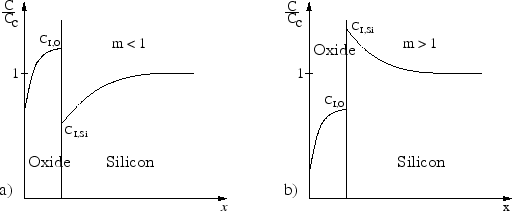
\includegraphics[width=0.75\linewidth]{img349.png}
	\caption{Schematic illustration of dopant redistribution}
	\label{graph_figure}
\end{figure}
\begin{table}[H]
	\centering
	\begin{tabular}{|c|c|c|c|c|c|}
		\hline
		Dopant species &
		Boron &
		Phosphor &
		Antimon &
		Arsen &
		Gallium \\
		\hline
		$m$ &
		0.1-0.3 &
		10 &
		10 &
		10 &
		20 \\
		\hline
	\end{tabular}
	\caption{Segregation coefficients $m$ for important dopant species in silicon}
	\label{table_diffusion_coeff}
\end{table}
\newpage
\section{MOS Capacitance}
\url{https://ecee.colorado.edu/~bart/book/book/chapter6/ch6_3.htm}

\subsection{Threshold voltage ($V_T$)}
The formula for calculating the threshold voltage of a MOS device is the following:
\begin{equation}
V_T = V_{t-mos} + V_{FB}
\end{equation}
where $V_{t-mos}$ is the threshold voltage of an ideal MOS capacitor, $V_{FB}$ is the flat-band voltage and $V_{t-mos}$ is the threshold.
The MOS threshold voltage, $V_{t-mos}$ is calculated by considering the MOS capacitor structure that form the gate of the MOS transistor.

The ideal threshold voltage may be expressed as:
\begin{equation}
V_{t-mos}=2 \phi_F + \frac{Q_b}{C_{ox}}
\end{equation}
\begin{equation}
Q_b
=
\sqrt{2 \epsilon_{Si} \cdot q \cdot N_{implant}  \cdot  ( \left| 2 \phi_F \right| + V_{SB}) }
\end{equation}
where $C_{ox}$ is the oxide capacitance and $Q_b$ which is called the bulk charge term.\\

The bulk potential is given by:
\begin{equation}
\phi_F
=
V_{th} \cdot ln\left(\frac{p}{N_i}\right)
=
V_{th} \cdot ln\left(\frac{N_i}{n}\right)
\end{equation}

$V_{th}$ is the thermal voltage.\footnote{\url{https://en.wikipedia.org/wiki/Boltzmann_constant\#Role_in_semiconductor_physics:_the_thermal_voltage}}
\begin{equation}
V_{th} = \frac{k T}{q} \approx 0.026 \frac{J}{C} = 0.026 V = 26mV
\end{equation}
With the variables being:
\begin{itemize}
\item $k=1.38064852\cdot 10^{-23}  \frac{J}{K}$ is the Boltzmann constant
\item $q=1.602 \cdot 10^{-19} C$ is the elementary charge
\item $T= 300 K$ the temperature, which we assume to be the room temperature for simplicity further on in this document as well.
\end{itemize}

\begin{mdframed}[linewidth=2pt,linecolor=red]
We can directly switch $\frac{J}{C}$ with Volts because these two units are equal!\footnote{\url{https://en.wikipedia.org/wiki/Volt}}
Also $V_{th}$ will be treated as a constant for any further calculations within this document.\\

The same goes for the $eV$ to $V$ conversion, wherever we have work functions to potentials because (e.g. $\Phi_M$ for Aluminum):
$4.1 eV \approx 6.56892414528 10^{-19}J$ \\
$\Phi_M=\frac{E_M}{q}=\frac{4.1 eV}{q}=\frac{6.56892414528 10^{-19} J}{q} = \frac{6.56892414528 10^{-19} J}{1.602176634 10^{-19} C} \approx 4.099999966220953 \frac{J}{C} = \underline{4.1V}$ \\
\end{mdframed}

Since we connect bulk and source $V_{SB}=0$ we can simplify the equation to become
\begin{equation}
Q_b
=
\sqrt{2\cdot\epsilon_{Si}\cdot q\cdot N_{implant} \cdot  ( \left| 2 \cdot \phi_F \right|) }
\end{equation}
\begin{equation}
Q_b
=
2\cdot\sqrt{\epsilon_{Si}\cdot q\cdot N_{implant}\cdot \left| \phi_F \right| }
\end{equation}


$V_{FB}$, is given by:
\begin{equation}
V_{FB}
=
\phi_{MS}-\frac{Q_SS}{C_{ox}}-\frac{1}{C_{ox}}\int_{0}^{t_{ox}}\frac{x}{x_{ox}}\rho(x) dx
\end{equation}

Because we're not yet dealing with non-volatile memory devices which contain an oxide surface state charge we can just $\rho(x)=0$.
$Q_{SS}$ is a value which has to be measured.

\begin{equation}
V_{FB}
=
\phi_{MS} - \frac{Q_{SS}}{C_{ox}}
\end{equation}
with
\begin{equation}
V_{FB}
=
\phi_{MS} - \frac{Q_{SS}}{C_{ox}}
=
\phi_{M} - \phi_{S} - \frac{Q_{SS}}{C_{ox}}
=
\phi_{M} -  \left(\chi + \frac{E_g}{2 q} + \phi_F \right) - \frac{Q_{SS}}{C_{ox}}
\end{equation}

And because of the simplifications we did to $F_{FB}$ which essentially led to $F_{FB}=\phi_{MS}$ we get to:
\begin{equation}
V_T = V_{t-mos} + \phi_{MS}
\end{equation}
\begin{equation}
V_T = 2 \phi_F + \frac{Q_b}{C_{ox}} + \phi_{MS}
\end{equation}
\begin{equation}
V_T = 2 \phi_F + \frac{2 \sqrt{\epsilon_{Si}\cdot q\cdot \left| \phi_F \right| \cdot N_{implant} }}{C_{ox}} + \phi_{MS}
\end{equation}
\begin{equation}
V_T = 2 \phi_F + \frac{2 \sqrt{\epsilon_{Si}\cdot q\cdot \left| \phi_F \right| \cdot N_{implant} }}{C_{ox}} + \phi_{M} -  \left(\chi + \frac{E_g}{2 q} + \phi_F \right) - \frac{Q_{SS}}{C_{ox}}
\end{equation}
\begin{equation}
V_T = 2 \phi_F + \frac{2 \sqrt{\epsilon_{Si}\cdot q\cdot \left| \phi_F \right| \cdot N_{implant} }}{C_{ox}} + \phi_{M} -  \chi - \frac{E_g}{2 q} - \phi_F - \frac{Q_{SS}}{C_{ox}}
\end{equation}
\begin{equation}
V_T = \phi_F + \frac{2 \sqrt{\epsilon_{Si}\cdot q\cdot \left| \phi_F \right| \cdot N_{implant} }}{C_{ox}} + \phi_{M} -  \chi - \frac{E_g}{2 q} - \frac{Q_{SS}}{C_{ox}}
\end{equation}

With the variables and constants being the following we now can put the formula together:
\begin{itemize}
\item $N_i$ is the carrier concentration in intrinsic (undoped) silicon. $N_i$ is equal to $1.45 \times 10^{10} cm^{-3} = 1.45 \times 10^{16} m^{-3}$ at 300\degree K
\item $Q_{SS}$ depends on the process and is measured. Usually it's between $10^{9}\frac{1}{cm^2}$ and $10^{10}\frac{1}{cm^2}$ ergo  $Q_{SS} = q \cdot 10^{10}\frac{1}{cm^2} = 1.6 \cdot 10^{-5}\frac{C}{m^2}$
\item $E_M = q\cdot\phi_M = 4.1 eV$ is the "work function" of our metal at the gate (Aluminum)
\item $E_g=E_g(300) [eV]$ \\
$E_g(T) = E_g(0) - \frac{\alpha T^2}{T+\beta} = 1.166 - 4.73 \cdot 10^{-4} \cdot \frac{T^2}{T+636} [eV]$ is the band gap energy of silicon at a given temperature\footnote{\url{https://ecee.colorado.edu/~bart/book/eband5.htm}} for which the parameters can be taken from \autoref{band_gap_parameters}
\begin{table}[H]
\centering
\begin{tabular}{|c|c|c|c|}
\hline
{} &
\textbf{Germanium} &
\textbf{Silicon} &
\textbf{GaAs} \\
\hline
$Eg(0) [eV]$ &
0.7437 &
1.166 &
1.519 \\
\hline
$\alpha [eV/K]$ &
4.77 x 10-4 &
4.73 x 10-4 &
5.41 x 10-4 \\
\hline
$\beta [K]$ &
235 &
636 &
204 \\
\hline
\end{tabular}
\caption{Band cap energy parameters}
\label{band_gap_parameters}
\end{table}
\item $C_{ox} \left[\frac{F}{m^2}\right]$ is the capacity of the gate oxide
\item $\epsilon_0 = 8.85 \cdot 10^{-14} \frac{F}{cm}.= 8.85 \cdot 10^{-12} \frac{F}{m} $ is the electric permittivity in vacuum
\item $\epsilon_{Si} =11.68 \cdot \epsilon_0$ is the relative permittivity of silicon
\item $\epsilon_{ox} = 3.9 \cdot \epsilon_0$ is the relative permittivity of silicon oxide
\item $t_{ox} [cm]$ is the thickness of the oxide layer in cm
\item $E_{ef} = q \cdot \chi = 4.05 eV$ is the electron affinity of a silicon crystal surface\footnote{\url{https://en.wikipedia.org/wiki/Electron_affinity}}
\item $q=1.602 \cdot 10^{-19} C$ is the elementary charge
\end{itemize} 

The contact potential from the Aluminum contact to the surface of the gate (silicon below the oxide) is fixed for $T=300\degree K$:
\begin{equation}
\phi_{M} -  \chi - \frac{E_g}{2 q} = 4.1V - 4.05V - \frac{1.12eV}{2 q} = 4.1V - 4.05V - 0.56V = -0.51V
\end{equation}

From that we get
\begin{equation}
V_T = \phi_F + \frac{2 \sqrt{\epsilon_{Si}\cdot q \cdot \left| \phi_F \right| \cdot N_{implant} }}{C_{ox}} - 0.51V
\end{equation}

Now we can calculate the thresholds for P substrate ($V_{Tp}$) and N substrate  ($V_{Tn}$), respectively the wells we build on unpredoped substrated, which makes the equation for single-doped substrate valid for both wells with
\begin{equation}
\phi_{Fn}
=
V_{th} \cdot ln\left(\frac{N_i}{N_{implant}}\right)
\end{equation}
\begin{equation}
\phi_{Fp}
=
V_{th} \cdot ln\left(\frac{N_{implant}}{N_i}\right)
\end{equation}

Which brings us to the equations for the N-channel and P-channel thresholds:

(N-Channel MOSFETs are built on p-substrate)
\begin{equation}
V_{Tn} = \phi_{Fp} + \frac{2 \sqrt{\epsilon_{Si}\cdot q \cdot \left| \phi_{Fp} \right| \cdot N_{implant} }}{C_{ox}} - 0.51V
\end{equation}

(P-Channel MOSFETs are built on n-substrate)
\begin{equation}
V_{Tp} = \phi_{Fn} + \frac{2 \sqrt{\epsilon_{Si}\cdot q \cdot \left| \phi_{Fn} \right| \cdot N_{implant} }}{C_{ox}} - 0.51V
\end{equation}

The threshold voltage dependence on the doping density is illustrated with \autoref{img:overview_doping_threshold} for both n-type and p-type MOSFETs with an aluminum gate metal.
\begin{figure}[H]
	\centering
	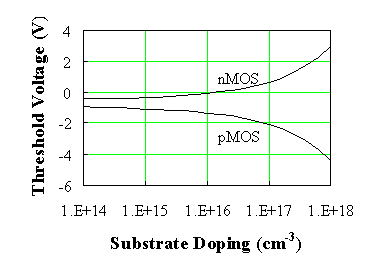
\includegraphics[scale=0.5]{doping_thresholds_overview.png}
	\caption{Threshold voltage of n-type (upper curve) and p-type (lower curve) MOSFETs versus substrate doping density.}
	\label{img:overview_doping_threshold}
\end{figure}

This equation will be used further on to find the optimum gate oxide thickness for our transistors.



\subsection{The substrate bias effect}
\section{Threshold voltage ($V_T$) adjustment}
At some point in the future this will be of very high relevance, because the lower the size of the transistors becomes, the higher the offset to $V_{Tp}$ and $V_{Tn}$ needs to be in order to stay on TTL 5V logic level, or at least compensate for the lowered voltages in order to reach the 3.3V CMOS logic levels.

Adjustment of the threshold voltage can be achieved by:
\begin{itemize}
\item A relatively small dose $N_I$ (units: ions/$cm^2$) of dopant atoms is implanted into the near-surface  region of the semiconductor.
\item When the MOS device is biased in depletion or inversion, the implanted dopants add to (or substract from) the depletion charge near the oxide-semiconductor interface
\end{itemize}

The formula to calculate the voltage offset is:
\begin{equation}
\Delta V_T = -\frac{q N_I}{C_{ox}} 
\left\{\begin{matrix}
N_I > 0\ for\ donor\ atoms\ (Phosporus/N) \\
N_I < 0\ for\ acceptor\ atoms\ (Boron/P)
\end{matrix}\right.
\end{equation}

\newpage
\section{Chemistry}
\subsection{Etching silicon dioxide}
A very "selective" chemical for SiO2 - i.e. does not etch silicon at all - is hydrofluoric acid (HF). If used directly such etchant has a too fast and aggresive action on the oxide, making very difficult the undercut and the linewidth control. For such reason, HF is universally used as a "buffered" solution, which can keep the etch rate low and constant, by moderating the PH level of the bath. This allows the etching time to be reliably correlated to the etching depth.

The industry standard buffered hydrofluoric acid solution (BHF\label{BHF}) has the following formulation:
\begin{itemize}
	\item 6 volumes of ammonium floride (NH4F, 40\% solution)
	\item 1 volume of HF.
\end{itemize}
This can be prepared, for example, by mixing 113 g of NH4F in 170 ml of H2O, and adding 28 ml of HF.\\
The etch rate at room temperature can range from 1000 to 2500 Å/min (100-250nm/min).
This depends on the actual density of the oxide which, as an amorphous layer, can have a more compact structure (if thermally grown in is oxygen) or less compact (if grown by CVD).
The following etching reaction holds:
\begin{equation}
	SiO_2 + 6HF \rightarrow H_2SiF_6 + H_2O
\end{equation}\\
where $H_2SiF_6$ is water soluble.\\
A common buffered oxide etch solution comprises a 6:1 volume ratio of 40\% NH4F in water to 49\% HF in water. This solution will etch thermally grown oxide at approximately 2 nanometres per second at 25 degrees Celsius.\label{BHF_six_to_one}
\footnote{Wolf, S.; R.N. Tauber (1986). Silicon Processing for the VLSI Era: Volume 1 - Process Technology. pp. 532–533. ISBN 978-0-9616721-3-3} \\

Another popular etching formulation is the P-etch:

60 volumes of $H_2O$ + 3 vol. of HF + 2 vol. of $HNO_3$, that is: 300 ml of $H_2O$ + 15 ml of HF + 10 ml of $HNO_3$.

The P-etch action is strongly dependent on oxide density, as it results from the growth technique.
An example is reported in the literature\footnote{A. Pliskin, J.Vac.Sci Technol., vol. 14, p.1064, 1977}, indicating 120 Å/min for thermal oxide and 250-700 Å/min for sputtered oxide.

A slow etching bath is preferred for opening mask windows for a silicon substrate.
However, the etching process could be used just for removing the oxide film from the whole surface.
In this case the etching speed is not critical, and a fast solution can be used, such as HF diluited 1:10 in water.
The etching time can be easily evaluated by visually inspecting the surface.
Once the oxide film is removed, the metal-grey color of the silicon surface appears.

Sometimes a very light etch is required, for removing just a few atomic layers.
This is the case of surface cleaning and decontamination. HF diluited 1 : 50 in water can be used.
The etching speed will be around 70 Å / min. For example, a typical 50 Å "native" oxide on silicon can be removed with a 45 - 50 sec light etch.

\newpage

\subsection{Etching silicon nitride}
Thin films made of amorphous silicon nitride ($Si_3N_4$) are usually deposited by chemical vapour deposition from silane ($SiH_4$) and ammonia ($NH_3$).
Since they act as a barrier for water and sodium, they have a major role as passivation layers in microchip fabrication.
Patterned nitride layers are also used as a mask for spatially selective silicon oxide growth, and as an etch mask when $SiO_2$ masks cannot be used.

One example of the latter situation is given by the anisotropic etching of silicon in KOH.
The etching rate of $SiO_2$ in KOH is nearly 1000 times slower than the etching rate of silicon, and in most cases a $SiO_2$ mask can be used successfully.
However, a very deep selective etch may require a long etching time, and the 1000:1 etching rate ratio may result still too small to prevent the $SiO_2$ mask from being etched off before the process is completed.
In this circumstance $Si_3N_4$, thanks to its reduced etched rate, can successfully replace the oxide mask layer.

The wet etching of nitride films is often performed in concentrated hot orthophosphoric acid ($H_3PO_4$).
The bath temperature can range from 150°C to 180°C (boiling point) with a corresponding etch rate between 10 and 100 Å/min.
It is good practice to bring the vapours into contact with a cold surface and to drive the condensed liquid back into the etching bath.
This technique is referred to as "reflux".

The etching rates of silicon nitride, silicon oxide, and silicon in $H_3PO_4$ are respectively in the 50 : 5 : 1 ratio.
\section{Growing silicon nitride}\label{chemistry_growing_nitride}
In order to grow a high quality layer of silicon nitride on top of a silicon wafer which is adapted to be patterned and to serve as a mask for diffusion or implantation of selected impurities, the wafer is best put into a chamber evacuated to a pressure less than about 1 Torr and heated between 650 and 900 \degree C.
A gaseous mixture comprising primarily of ammonia and a silicon compound, having a ratio of relative concentrations in the range on 4:1 and 20:1 \footnote{\url{http://www.freepatentsonline.com/4395438.html}}, is flooded into that chamber with a silicon compound flow rate of greater than approximately 12 cubic centimeters per minute.
The growth rate will be around 50 Angstroms per minute.
That setup is called Low-Pressure Chemical Vapor Deposition (LPCVD), which is commonly available in basically any semiconductor manufacturing plant or laboratory.

\newpage
\section{Process design}
We need to optimize our process to be TTL compatible (5V logic levels) and at the same time being as fast and power efficient as possible.
In order to have a good propagation delay with a technology node of around $1\mu m$ we will have to have gates with up to four stacked MOS transistors.

Acceptable input signal voltages range from 0 volts to 0.8 volts for a low logic state, and 2 volts to 5 volts for a high logic state.
Acceptable output signal voltages shall range from 0 volts to 0.5 volts for a low logic state, and 2.7 volts to 5 volts for a high logic state\footnote{\url{https://www.allaboutcircuits.com/textbook/digital/chpt-3/logic-signal-voltage-levels}}

\begin{figure}[H]
	\centering
	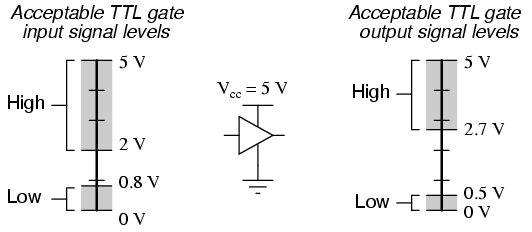
\includegraphics[scale=0.5]{logic_levels.png}
	\caption{TTL logic levels}
	\label{TTL_logic_levels}
\end{figure}

As shown in \autoref{TTL_logic_levels} we have some margin to make our PMOS and NMOS transistors work with each other in order to form a CMOS circuit which is actually working without getting warm.

Or more clearly defined
\begin{equation}
V_{off} \leq 0.8V
\end{equation}
and
\begin{equation}
V_{on} \geq 2V
\end{equation}
which are limits, elementary to our design.

\begin{figure}[H]
	\centering
	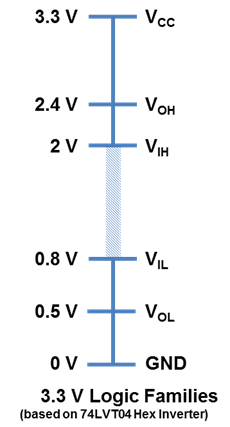
\includegraphics[scale=0.5]{cmos_3v3.png}
	\caption{CMOS 3.3V logic levels}
	\label{CMOS_logic_levels}
\end{figure}

This means that we also will be compatible to CMOS logic level output pins since their ON/OFF levels are within our tolerance range\footnote{\url{https://learn.sparkfun.com/tutorials/logic-levels/33-v-cmos-logic-levels}} as it is shown in \autoref{CMOS_logic_levels}.

We target threshold voltages of $V_{Tn} \approx 0.8V$ and $V_{Tp} \approx -0.8V$ which should be enough.
We can internally always shift the voltage supply levels to compensate for threshold variations.\footnote{Hagen! Please explain this part here}
\input{process_design_requirements.tex}
\subsection{Substrate}
For this process p-substrate is being used, but forks and modifications will be very well possible based on a Graphene substrate or alike, still under the LSPL.
The starting material is a p-type, <100> oriented silicon with a doping concentration of $\approx 9\times10^{14}cm^{-3}$.\\

\textbf{Reasons for using p-substrate}:\begin{itemize}
\item We can't use two different substrates for our design because in the design both PMOS and NMOS is present.
We have to choose which is more beneficial from fabrication point of view.
In general or say it's true that NMOS devices are always more in the Semiconductor Industry in comparison to PMOS devices.
For your reference-SRAM requires 6 transistors (4 NMOS, 2 PMOS).
\item Another reason for more number of NMOS is because of difference of mobility of electron and holes.
Electron mobility is almost twice of holes mobility and because of this ON-RESISTANCE of n-channel device is half of p-channel device with the same geometry and under the same operating conditions.
That means to achieve same impedance size of n-channel transistors is almost half of p-channel devices.
Same thing I can say in the different way that for same size of wafer, we can have more number of NMOS (means can perform more logical operation) in comparison to PMOS.
\end{itemize}
\subsection{Isolation}
For the isolation (\autoref{sti})  in this design the STI approach is being chosen.
Shallow trench isolation (STI), also known as box isolation technique, is an integrated circuit feature which prevents electric current leakage between adjacent semiconductor device components.\footnote{\url{https://www.google.com/patents/US7985656}}
STI is generally used on CMOS process technology nodes of 250 nanometers and smaller.\\

\textbf{Reasons for using box isolation}:\begin{itemize}
\item We want to be forward compatible to future LibreSilicon nodes with a size of 100nm or smaller
\item It simplifies the construction of the gate and allows us to use Aluminum instead of Polysilicon for the gate contact
\end{itemize}

\subsection{Interconnect}
The interconnects and the gate electrode are being made using Aluminum which is a very commonly used material to do interconnects in low-frequency and low-resolution applications \\

\textbf{Reasons for using Aluminum}:\begin{itemize}
\item It's a well explored material for interconnect with a lot of literature on how to process it
\item Aluminum is easy to etch compared to copper
\item It isn't contaminating everything like copper does and doesn't require special separated setup for handling
\item The machines at HKUST can do CMP for copper only on 4 inch wafers which would limit us in wafer size
\end{itemize}

\begin{mdframed}[linewidth=2pt,linecolor=green]
As soon as we've got CMOS all figured out, we will tackle copper interconnect in release 2.0
\end{mdframed}
\subsection{MOS gate}
The wires and the MOS gates can be modeled as an RC low-pass filter, for that reason the time constant $\tau=RC$ is limiting the clock frequency of our CMOS circuitry.
However, we can't just make the gate ultra thin, because lowered capacity also creates lowered thresholds, which will be a very big problem, as soon as we go into the 100nm range and lower.

In \autoref{nmos_gate_dimensioning} we defined the capacity of the gate to be $C_{ox} \leq 305.7 \frac{nF}{cm^2}$ which leads to the oxide capacity-thickness constraint with the variables being:
\begin{itemize}
\item $\epsilon_0 = 8.85 \cdot 10^{-14}\frac{F}{cm}. $ is the electric permittivity in vacuum
\item $\epsilon_{ox} =3.9 \cdot \epsilon_0$ is the relative permittivity of silicon dioxide
\end{itemize}
and the constraint being for the oxide thickness which is only silicon dioxide for now
\begin{equation}
C_{ox}
=
\frac{\epsilon_{ox}}{t_{ox}}
\end{equation}
\begin{equation}
t_{ox}
=
\frac{\epsilon_{ox}}{C_{ox}}
\end{equation}

And with numbers we get
\begin{equation}
t_{ox}
=
\frac{3.9 \cdot 8.85 \cdot 10^{-14}\frac{F}{cm}}{305.7 \frac{nF}{cm^2}}
=
1.129 \cdot 10^{-6} cm
=
11.29nm
\end{equation}

That's still doable with a precision high enough when using dry oxidation and a temperature of 1000\degree Celsius.
\subsection{NMOS threshold}\label{nmos_dimensioning}
First we take a look at the worst case of 4 stacked NMOS transistors, which is the highest stacking amount which will be possible in technologies relying on this process.

%%  ************    LibreSilicon's StdCellLibrary   *******************
%%
%%  Organisation:   Chipforge
%%                  Germany / European Union
%%
%%  Profile:        Chipforge focus on fine System-on-Chip Cores in
%%                  Verilog HDL Code which are easy understandable and
%%                  adjustable. For further information see
%%                          www.chipforge.org
%%                  there are projects from small cores up to PCBs, too.
%%
%%  File:           StdCellLib/Documents/LaTeX/schematic_AND4.tex
%%
%%  Purpose:        Schematic File for AND4
%%
%%  ************    LaTeX with circdia.sty package      ***************
%%
%%  ///////////////////////////////////////////////////////////////////
%%
%%  Copyright (c) 2018 by chipforge <hsank@nospam.chipforge.org>
%%  All rights reserved.
%%
%%      This Standard Cell Library is licensed under the Libre Silicon
%%      public license; you can redistribute it and/or modify it under
%%      the terms of the Libre Silicon public license as published by
%%      the Libre Silicon alliance, either version 1 of the License, or
%%      (at your option) any later version.
%%
%%      This design is distributed in the hope that it will be useful,
%%      but WITHOUT ANY WARRANTY; without even the implied warranty of
%%      MERCHANTABILITY or FITNESS FOR A PARTICULAR PURPOSE.
%%      See the Libre Silicon Public License for more details.
%%
%%  ///////////////////////////////////////////////////////////////////
    \begin{figure}[H]
	\centering
            \begin{circuitdiagram}{50}{33}
            \pin{2}{2.5}{L}{A}  % pin A, n-channel below
            \pin{2}{8.5}{L}{B}  % pin B, n-channel middle
            \pin{2}{14.5}{L}{C} % pin C, n-channel middle
            \pin{2}{20.5}{L}{D} % pin D, n-channel above
            \pin{2}{29.5}{L}{A} % pin A, p-channel left
            \pin{14}{29.5}{L}{B} % pin B, p-channel middle
            \pin{26}{29.5}{L}{C} % pin C, p-channel middle
            \pin{38}{29.5}{L}{D} % pin D, p-channel right
            \trans{nenh*}{6}{4}{R}{}{}  % nmos below
            \trans{nenh*}{6}{10}{R}{}{} % nmos middle
            \trans{nenh*}{6}{16}{R}{}{} % nmos middle
            \trans{nenh*}{6}{22}{R}{}{} % nmos above
            \trans{nenh*}{54}{22}{R}{}{} % nmos inverter
            \trans{penh*}{6}{28}{R}{}{} % pmos left
            \trans{penh*}{18}{28}{R}{}{} % pmos middle
            \trans{penh*}{30}{28}{R}{}{} % pmos middle
            \trans{penh*}{42}{28}{R}{}{} % pmos right
            \trans{penh*}{54}{28}{R}{}{} % pmos inverter
            \wire{8}{6}{8}{8}     % wire between nmos
            \ground{8}{0.5}{D}  % ground below nmos
            \ground{56}{18.5}{D}  % ground below inverter
            \power{8}{31.5}{U}{}  % power above left pmos
            \power{20}{31.5}{U}{}  % power above middle pmos
            \power{32}{31.5}{U}{}  % power above middle pmos
            \power{44}{31.5}{U}{}  % power above right pmos
            \power{56}{31.5}{U}{}  % power above inverter
            \wire{8}{12}{8}{14}     % wire between nmos
            \wire{8}{18}{8}{20}     % wire between nmos and pmos
            \wire{20}{25}{20}{26}
            \wire{32}{25}{32}{26}
            \wire{44}{25}{44}{26}
            \wire{8}{25}{51}{25}    % wire before inverter gate
            \junct{8}{25}
            \junct{20}{25}
            \junct{32}{25}
            \junct{44}{25}
            \junct{56}{25}
            \wire{51}{29.5}{51}{20.5}   % wire at inverter gates
            \junct{51}{25}
            \wire{56}{25}{58}{25}    % wire before pin Z
            \pin{59}{25}{R}{Z}  % pin Z
            \end{circuitdiagram}
            \caption{AND4 gate}
    \end{figure}
As shown in  \autoref{TTL_logic_levels} our acceptable voltages for our CMOS "ON" state range from 2V to VDD (which typically is around $5V\pm0.25V$)

\begin{equation}
V_{on} \geq 2V
\end{equation}

Because there are four transistors dividing the voltage by being in series, the power supply voltage is being divided by the amount of transistors in series.
In order to match the threshold voltages of all of the transistors, which is needed for a working digital logic, the following equation need to be satisfied

\begin{equation}
V_{on} > 4 \cdot V_{Tn}
\end{equation}

Lets assume the worst case with

\begin{equation}
V_{on} = 2V
\end{equation}

Which leads to the required worst case threshold tolerance value

\begin{equation}
4 \cdot V_{Tn} < 2V
\Rightarrow
V_{Tn} < 500mV
\end{equation}
 
With the values derived from \autoref{gate_dimensioning} and a surface concentration for our P-well of $10^{22}\frac{1}{m^3}$ we are already set because $\approx 0.39V$ are already better than we need.

We target a concentration of $N_p = 10^{16}\frac{1}{cm^3}=10^{22}\frac{1}{m^3}$.

The depletion zone thickness at its peak will be $W_{dmax} \approx 2.73 \cdot 10^{-7} m = 273 nm$

With an implantation (or constant source diffusion step), we can now set a range/energy and dosage in order to cover the depletion zone area.

For getting the energy and dose we look at \autoref{graphics_range_and_straggle} or use the web tool linked in the implant chapter.

The depth of the p-well $\approx 2 \mu m$ comes mainly from the need to fulfill the condition from \autoref{physics_drive_in}

\begin{equation}
x_e = 2 \cdot \sqrt{D_e \cdot t_e} \gg 2 \cdot \sqrt{D_v \cdot t_v} = x_v
\end{equation}

\newpage

We already got the background ($N_B \approx 7 \cdot 10^{14} \frac{1}{cm^3}=7 \cdot 10^{20} \frac{1}{m^3}$) concentration from the specs of the basis substrate.

\begin{equation}
N_p - N_B = 10^{22}\frac{1}{m^3} - 7 \cdot 10^{20} \frac{1}{m^3} = 9.3 \cdot 10^{21} \frac{1}{m^3}
\end{equation}

We use a drive in temperature of $1150 \degree C$ which is  $T = 1423.15 \degree K$ in Kelvin which gives us the diffusion coefficient $D=9.1 \cdot 10^{-17}  \frac{m^2}{s}$

Now using
\begin{equation}
N(x,t)
=
\frac{Q}{\sqrt{\pi\cdot D \cdot t}} \cdot \exp\left(\frac{-x^2}{4 \cdot D \cdot t}\right)
\end{equation}

We set the conditions and get the required diffusion time as well as the initial dosage in one shot:
\begin{equation}
N(0,t)
=
\frac{Q}{\sqrt{\pi\cdot D \cdot t}}
=
N_p-N_B
=
7 \cdot 10^{20} \frac{1}{m^3}
\end{equation}
\begin{equation}
x
=
2 \cdot \sqrt{D \cdot t}
=
2 \mu m
=
2 \cdot 10^{-6} m
\end{equation}
\begin{equation}
\Rightarrow
t \approx 11018s \approx \underline{3h}
\end{equation}
\begin{equation}
\Rightarrow
Q
=
7 \cdot 10^{20} \frac{1}{m^3} \cdot \sqrt{\pi\cdot D \cdot t}
\approx
\underline{1.64 \cdot 10^{16} \frac{1}{m^2}}
\end{equation}

If we plot the functions from our calculation we can yield the below graphics\footnote{see simulation/diffusion\_pwell.wxmx}

\begin{figure}[H]
	\centering
	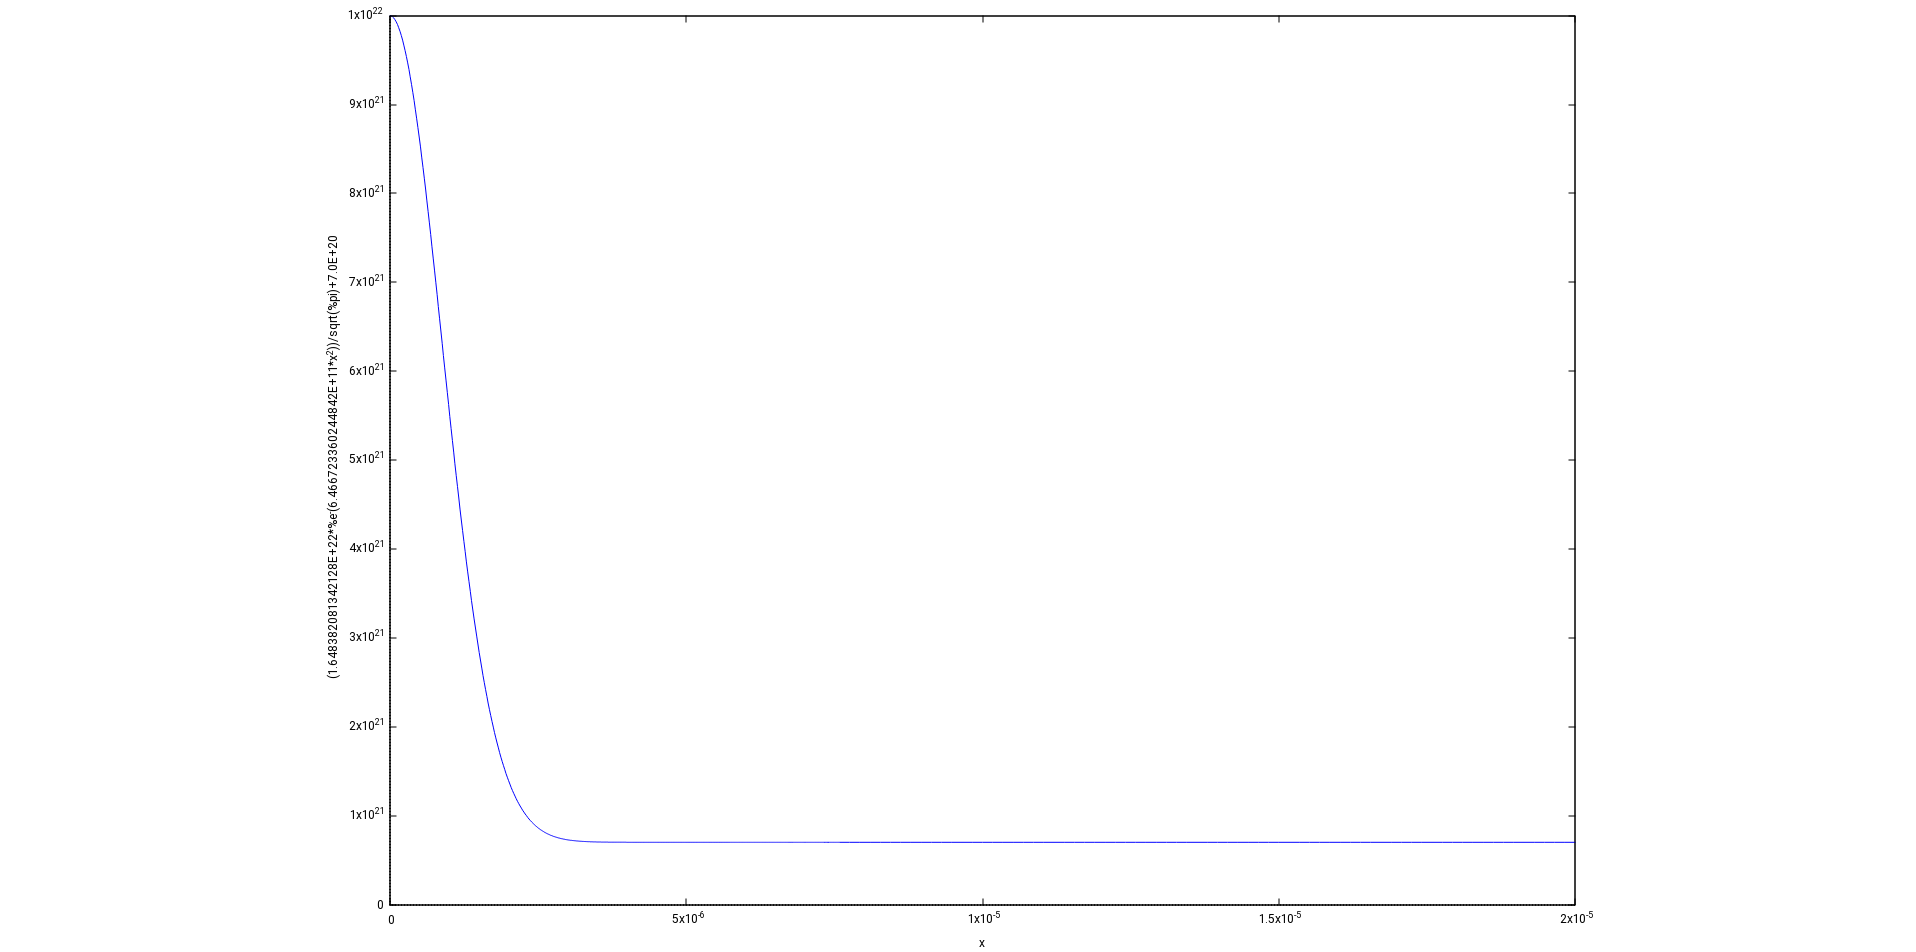
\includegraphics[width=0.75\textwidth]{p-well-diffusion.png}
	\caption{Dopant concentration after 3 hours}
	\label{pwell_drive_in_outcome}
\end{figure}

In \autoref{pwell_drive_in_outcome} we can see that after three hours we already have the desired even gradient which and deep penetration of dopants, which will give us a low $R_{DS}$.
\subsection{PMOS threshold}
Now we take a look at the worst case of 4 stacked PMOS transistors, which is the highest stacking amount which will be possible in technologies relying on this process.
%%  ************    LibreSilicon's StdCellLibrary   *******************
%%
%%  Organisation:   Chipforge
%%                  Germany / European Union
%%
%%  Profile:        Chipforge focus on fine System-on-Chip Cores in
%%                  Verilog HDL Code which are easy understandable and
%%                  adjustable. For further information see
%%                          www.chipforge.org
%%                  there are projects from small cores up to PCBs, too.
%%
%%  File:           StdCellLib/Documents/LaTeX/schematic_OR4.tex
%%
%%  Purpose:        Schematic File for OR4
%%
%%  ************    LaTeX with circdia.sty package      ***************
%%
%%  ///////////////////////////////////////////////////////////////////
%%
%%  Copyright (c) 2018 by chipforge <hsank@nospam.chipforge.org>
%%  All rights reserved.
%%
%%      This Standard Cell Library is licensed under the Libre Silicon
%%      public license; you can redistribute it and/or modify it under
%%      the terms of the Libre Silicon public license as published by
%%      the Libre Silicon alliance, either version 1 of the License, or
%%      (at your option) any later version.
%%
%%      This design is distributed in the hope that it will be useful,
%%      but WITHOUT ANY WARRANTY; without even the implied warranty of
%%      MERCHANTABILITY or FITNESS FOR A PARTICULAR PURPOSE.
%%      See the Libre Silicon Public License for more details.
%%
%%  ///////////////////////////////////////////////////////////////////
    
    \begin{figure}[H] %\caption{Schematic}
       \centering
            \begin{circuitdiagram}{60}{33}
            \pin{2}{2.5}{L}{A}  % pin A, n-channel left
            \pin{2}{11.5}{L}{A}  % pin A, p-channel below
            \pin{2}{17.5}{L}{B}  % pin B, p-channel middle
            \pin{2}{23.5}{L}{C} % pin C, p-channel above
            \pin{2}{29.5}{L}{D} % pin D, p-channel above
            \pin{14}{2.5}{L}{B} % pin B, n-channel middle
            \pin{26}{2.5}{L}{C} % pin C, n-channel right
            \pin{38}{2.5}{L}{D} % pin D, n-channel right
            \trans{nenh*}{6}{4}{R}{}{}  % nmos left
            \trans{penh*}{6}{10}{R}{}{} % pmos below
            \trans{penh*}{6}{16}{R}{}{} % pmos middle
            \trans{penh*}{6}{22}{R}{}{} % pmos above
            \trans{penh*}{6}{28}{R}{}{} % pmos above
            \trans{nenh*}{18}{4}{R}{}{} % nmos middle
            \trans{nenh*}{30}{4}{R}{}{} % nmos right
            \trans{nenh*}{42}{4}{R}{}{} % nmos right
            \wire{8}{6}{8}{8}     % wire between nmos
            \ground{8}{0.5}{D}  % ground below nmos
            \power{8}{31.5}{U}{}  % power above left pmos
            \ground{20}{0.5}{D}  % ground below nmos
            \ground{32}{0.5}{D}  % ground below nmos
            \ground{44}{0.5}{D}  % ground below nmos
            \wire{8}{12}{8}{14}     % wire between nmos
            \wire{8}{18}{8}{20}     % wire between nmos and pmos
            \wire{20}{7}{20}{6}
            \wire{32}{7}{32}{6}
            \wire{8}{7}{51}{7}    % wire before inverter gates
            \wire{51}{2.5}{51}{11.5}  % wire on inverter gates
            \junct{8}{7}
            \junct{20}{7}
            \junct{32}{7}
            \junct{44}{7}
            \junct{51}{7}
            \trans{nenh*}{54}{4}{R}{}{} % nmos right
            \trans{penh*}{54}{10}{R}{}{} % pmos below
            \power{56}{13.5}{U}{}  % power above left pmos
            \ground{56}{0.5}{D}  % ground below nmos
            \wire{56}{7}{58}{7}    % wire before pin
            \wire{56}{6}{56}{8}    % wire before pin
            \junct{56}{7}
            \pin{59}{7}{R}{Z}  % pin Z
            \end{circuitdiagram}
            \caption{OR4 gate}
    \end{figure}

\newpage
\section{Process steps}
\tikzstyle{block} = [rectangle, draw, fill=blue!20, text width=3cm, text centered, rounded corners, minimum height=1.5cm]
\tikzstyle{line} = [draw, very thick, color=black!50, -latex']

The general flow chart of the overall process flow can be seen in \autoref{full_flow}.
These process steps will be discussed within the following sections.
\begin{figure}[H]
	\centering
	\begin{tikzpicture}[node distance=2cm, thick,scale=0.8, every node/.style={transform shape}]
		%% Place nodes
		%active CMOS				
		\node [block] (isolation) at (4,20) {Isolation (STI)\\ \autoref{sti}};
		\node [block, below of=isolation] (nwell) {N-Well\\ \autoref{nwell_chapter}};
		\node [block, below of=nwell] (pwell) {P-Well\\ \autoref{pwell_chapter}};
		\node [block, below of=pwell] (gate) {Gate\\ \autoref{gate}};
		\node [block, below of=gate] (np) {n+ Implant\\ \autoref{nimplant}};
		\node [block, below of=np] (pp) {p+ Implant\\ \autoref{pimplant}};
		\node [block, below of=pp] (silicification) {Silicification\\ \autoref{step_silicification}};
		%post proces
		\node [block] (via1) at (8,8) {First vias\\ \autoref{via1}};
		\node [block, above of=via1] (metal1) {First metal\\ \autoref{metal1}};
		\node [block, above of=metal1] (via2) {Additional vias\\ \autoref{via2}};
		\node [block, above of=via2] (metal2) {Additional metal\\ \autoref{metal2}};
		\node (repeat) at (10.5,14.5) {Repeat};

		%% Draw edges
		\path [line] (isolation) -- (nwell);
		\path [line] (nwell) -- (pwell);
		\path [line] (pwell) -- (gate);
		\path [line] (gate) -- (np);
		\path [line] (np) -- (pp);
		\path [line] (pp) -- (silicification);
		\path [line] (silicification) -- (via1);
		\path [line] (via1) -- (metal1);
		\path [line] (metal1) -- (via2);
		\path [line] (via2) -- (metal2);
		\path [line] (metal2) -- +(3,0) -- +(3,-2) -- (via2);

		\draw[dotted] (2,6) rectangle (6,21);
		\node at (4,6.5) {CMOS process};
		\draw[dotted] (6,6) rectangle (12,21);
		\node at (8,6.5) {Interconnect};

		%\draw[dotted] (1.5,9) rectangle (10.5,21.5);
		%\node at (4,9.5) {Front-end processing};

		%\draw[dotted] (11,9) rectangle (15,21.5);
		%\node at (13,9.5) {Back-end processing};
	\end{tikzpicture}
	\caption{Frontend and backend process flow}
	\label{full_flow}
\end{figure}
The six overall process steps are part of an active part of the technology, while the final metal (respectively contact) layers will be used for making a contact between the logic gates and macro cells and making them available to the exterior world.

For this process p-substrate is the required basic substrate, but forks and modifications will be very well possible based on a Graphene substrate or alike, still under the LSPL.
The starting material is a p-type, <100> oriented silicon with a doping concentration of $\approx 9\times10^{14}cm^{-3}$.\\



\label{process_overview}
\newpage
\section{Shallow trench isolation}\label{sti_chapter}
The geometry of a substrate with STI implemented can be seen in \autoref{sti_target}.

\begin{figure}[H]
	\centering
	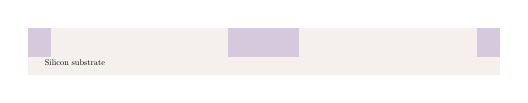
\begin{tikzpicture}[node distance = 3cm, auto, thick,scale=\CrossAndTopSectionBig, every node/.style={transform shape}]
		% substrate
\fill[substrate] (0,0) rectangle (20,2);
\node at (2,0.5) {Silicon substrate};
%trenches
\fill[isolationoxide] (0,0.75) rectangle (1,2);
\fill[isolationoxide] (8.5,0.75) rectangle (11.5,2);
\fill[isolationoxide] (19,0.75) rectangle (20,2);
	\end{tikzpicture}
	
\begin{tikzpicture}[node distance = 3cm, auto, thick,scale=\CrossAndTopSectionBig, every node/.style={transform shape}]
		% substrate
\fill[YellowOrange] (0,0) rectangle (20,12);
% trench area
\fill[DarkGray] (0,0) rectangle (1,12);
\fill[DarkGray] (8.5,0) rectangle (11.5,12);
\fill[DarkGray] (19,0) rectangle (20,12);
\fill[DarkGray] (0,0) rectangle (20,1.25);
\fill[DarkGray] (0,7.5) rectangle (20,12);
	\end{tikzpicture}
	\caption{Shallow trench isolation target geometry}
	\label{sti_target}
\end{figure}

As can be seen in \autoref{nwell_target}, the n-well and the STI trench are supposed to have approximately the same depth but the n-well and p-well go down a little bit further.
Because the n-well will be $\approx 4 \mu m$ in depth we have to match this with our trench depth.
I order to allow a sufficiently low resistance of the ESD diode but at the same time a sufficient isolation of between the standard cells a trade-ff has been done.
The targeted depth of the box isolation is $\approx 2 \mu m$.

\begin{figure}[H]
	\centering
	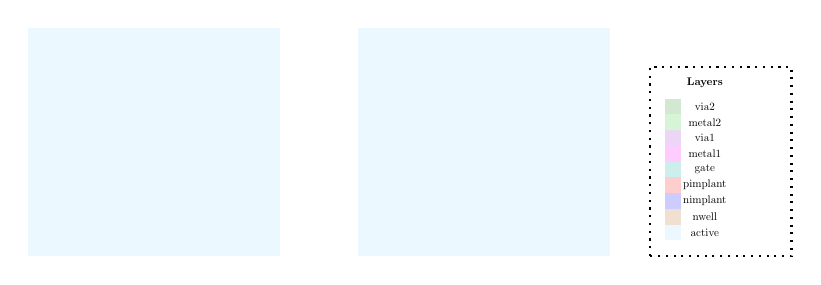
\begin{tikzpicture}[node distance =1cm, auto, thick,scale=\VLSILayout, every node/.style={transform shape}]
		\fill[nwell,opacity=0.2] (0.75,0.5) rectangle (8.75,7.75);
\fill[nwell,opacity=0.2] (11.25,0.5) rectangle (19.25,7.75);

\draw[dotted] (20.5,0.5) rectangle (25,6.5);

\node at (22.25,6) {\textbf{Layers}};

\fill[nwell,opacity=0.2] (21,1) rectangle (21.5,1.5);
\node at (22.25,1.25) {active};

\fill[resist,opacity=0.2] (21,1.5) rectangle (21.5,2);
\node at (22.25,1.75) {nwell};

\fill[blue,opacity=0.2] (21,2) rectangle (21.5,2.5);
\node at (22.25,2.25) {nimplant};

\fill[nitride,opacity=0.2] (21,2.5) rectangle (21.5,3);
\node at (22.25,2.75) {pimplant};

\fill[Emerald,opacity=0.2] (21,3) rectangle (21.5,3.5);
\node at (22.25,3.25) {gate};

\fill[Fuchsia,opacity=0.2] (21,3.5) rectangle (21.5,4);
\node at (22.25,3.75) {metal1};

\fill[DarkOrchid,opacity=0.2] (21,4) rectangle (21.5,4.5);
\node at (22.25,4.25) {via1};

\fill[LimeGreen,opacity=0.2] (21,4.5) rectangle (21.5,5);
\node at (22.25,4.75) {metal2};

\fill[ForestGreen,opacity=0.2] (21,5) rectangle (21.5,5.5);
\node at (22.25,5.25) {via2};

	\end{tikzpicture}
	\caption{Shallow trench isolation layout}
	\label{sti_layout}
\end{figure}

In \autoref{sti_layout} we can see the layout for the STI area.
The STI area will be everywhere, where no active areas are.
The field oxide needs to be grown out of trenches which can't been etched out of the silicon by using resist as a mask.
For that reason we will have to resort to a protective mask made from a silicon dioxide layer which has to be etched before hand.
So the mask will be exposed onto positive resist on top of the hard mask oxide layer in order to form a protective mask covering the active areas from having etched trenches into them..
After that we can either use a dry etching method or wet etching for cutting into the silicon substrate and making the active area become islands with trenches in between.
After these steps we have to remove the hard mask.
Our minimum width and height as well as the space between the active areas comes from the line space constrain of the silicon etcher and of course the optical limitations of the stepper which are as well 0.5\um.

\newpage

\subsection{Initial cleaning}
In order to remove the initial naturally grown silicon dioxide from the wafer, acid is being applied to the wafer which leads to a pure silicon substrate wafer as in the process illustration shown in \autoref{initial_cleaning}.

\begin{figure}[H]
	\centering
	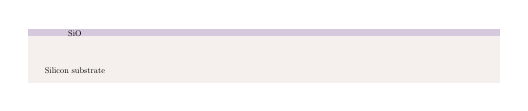
\begin{tikzpicture}[node distance = 3cm, auto, thick,scale=\CrossSectionOnly, every node/.style={transform shape}]
		% substrate
\fill[substrate] (0,0) rectangle (20,2);
\node at (2,0.5) {Silicon substrate};
% oxide
\fill[isolationoxide] (0,2) rectangle (20,2.3);
\node at (2,2.1) {SiO};
	\end{tikzpicture} \\
	
\includegraphics[scale=0.01]{down_arrow.png} \\
	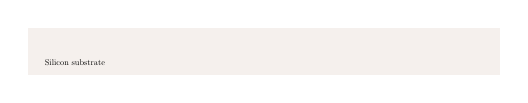
\begin{tikzpicture}[node distance = 3cm, auto, thick,scale=\CrossSectionOnly, every node/.style={transform shape}]
		% substrate
\fill[substrate] (0,0) rectangle (20,2);
\node at (2,0.5) {Silicon substrate};
	\end{tikzpicture}
	\caption{Initial cleaning}
	\label{initial_cleaning}
\end{figure}

This needs to be done because the naturally grown initially existing silicon oxide is not pure and may contain contamination which may render the final product unusable.

\subsubsection{Sulfuric Cleaning}
The sulfuric acid mixture, $H_2 S O_4 + H_2 O_2$ is being applied to the wafer for 10 minutes at a temperature of 120 \degree C.

\subsubsection{HF dip}
After the sulfuric cleaning a HF (HF:$H_2O$,1:50) dip is being performed for one minute. \\
Hydrofluoric acid (HF) is used to remove native silicon dioxide from wafers. Since it acts quickly, one needs to only expose the wafer for a short time ("dip").

\subsubsection{Drying}
After that the wafer needs to be dried and quickly processed further before new uncontrolled natural oxide can build up on the wafer through the contact with air.

\subsection{Hard mask: Oxide growth}
We need a thick layer of oxide as protective hard mask to etch the trenches into the silicon.

\begin{figure}[H]
	\centering
	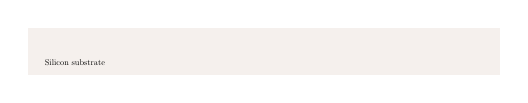
\begin{tikzpicture}[node distance = 3cm, auto, thick,scale=\CrossSectionOnly, every node/.style={transform shape}]
		% substrate
\fill[substrate] (0,0) rectangle (20,2);
\node at (2,0.5) {Silicon substrate};
	\end{tikzpicture} \\
	
\includegraphics[scale=0.01]{down_arrow.png} \\
	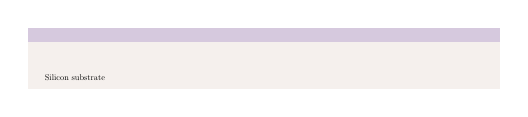
\begin{tikzpicture}[node distance = 3cm, auto, thick,scale=\CrossSectionOnly, every node/.style={transform shape}]
		% substrate
\fill[substrate] (0,0) rectangle (20,2);
\node at (2,0.5) {Silicon substrate};
\fill[isolationoxide] (0,2) rectangle (20,2.6);
	\end{tikzpicture}
	\caption{Hard mask growth}
\end{figure}

Because we want to etch 2\um deep into the silicon which takes 4 minutes and 30 seconds using KOH acid at 60\degreesC in \autoref{sti_trench_etch}.

This means the oxide layer needs to be at least 226 nm thick, so we choose a nice round number of 300nm.

The layer of silicon dioxide of around 300nm thickness is grown in wet ambient for 25 minutes at 1050\degreesC\footnote{\url{http://cleanroom.byu.edu/OxideTimeCalc}} in the diffusion furnace.

\newpage

\subsection{Hard mask: Patterning}

The resist is being deposited using spin coating and then baked depending on the baking time for the specific resist.

\begin{figure}[H]
	\centering
	\begin{tikzpicture}[node distance = 3cm, auto, thick,scale=\CrossSectionOnly, every node/.style={transform shape}]
		\input{tikz_process_steps/sti.hard_mask_oxide_growth.a.tex}
\fill[isolationoxide] (0,2) rectangle (20,2.6);
	\end{tikzpicture} \\
	
\includegraphics[scale=0.01]{down_arrow.png} \\
	\begin{tikzpicture}[node distance = 3cm, auto, thick,scale=\CrossSectionOnly, every node/.style={transform shape}]
		\input{tikz_process_steps/sti.hard_mask_oxide_growth.a.tex}
\fill[isolationoxide] (0,2) rectangle (20,2.6);
\fill[resist] (1,2.6) rectangle (8,3.2);
\fill[resist] (11.5,2.6) rectangle (19,3.2);
	\end{tikzpicture}
	\caption{Patterning with positive resist}
\end{figure}

The layout for being exposed onto the resist is being extracted from the "active" layer within the GDS2 file onto a dark field mask.

A dark field mask can be used because alignment doesn't play a role yet because it's the first layer, however the alignment crosses need to be included into the mask.

\subsection{Hard mask: Etching}\label{sti_mask_etch}

We open the access to the silicon outside of the active areas in order to etch the trenches.

\begin{figure}[H]
	\centering
	\begin{tikzpicture}[node distance = 3cm, auto, thick,scale=\CrossSectionOnly, every node/.style={transform shape}]
		\input{tikz_process_steps/sti.hard_mask_oxide_growth.b.tex}
\fill[resist] (1,2.6) rectangle (8,3.2);
\fill[resist] (11.5,2.6) rectangle (19,3.2);
	\end{tikzpicture} \\
	
\includegraphics[scale=0.01]{down_arrow.png} \\
	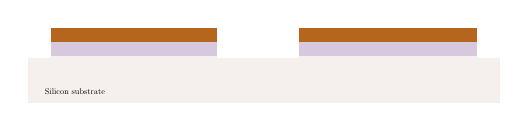
\begin{tikzpicture}[node distance = 3cm, auto, thick,scale=\CrossSectionOnly, every node/.style={transform shape}]
		% substrate
\fill[substrate] (0,0) rectangle (20,1.9);
\node at (2,0.5) {Silicon substrate};

% substrate islands
\fill[substrate] (1,1.9) rectangle (8,2);
\fill[substrate] (11.5,1.9) rectangle (19,2);

% pad oxide
\fill[isolationoxide] (1,2) rectangle (8,2.6);
\fill[isolationoxide] (11.5,2) rectangle (19,2.6);

% resist
\fill[resist] (1,2.6) rectangle (8,3.2);
\fill[resist] (11.5,2.6) rectangle (19,3.2);
	\end{tikzpicture}
	\caption{Nitride mask etching}
\end{figure}

There are dry etching and wet etching methods available for etching the oxide hard mask. The downside of wet etching is that it also etches horizontally, however the chemical BHF is readily available and allows for easy implementation of the process.\\

\textbf{Possible approaches}:
\begin{itemize}
	\item \textbf{"DRIE Etcher \#1" from HKUST} \\
	We can use anisotropic plasma etching for sharper borders.
	\item \textbf{Chemical solution} \\
	We can use buffered hydrofluoric acid (BOE (1:6)) at room temperature for a little bit over 3 minutes in order to get through the 300nm of oxide.\\
	Too long over 3 minutes might cause under-etch however!
\end{itemize}

\subsection{Hard mask: Resist removal}
Now we need to remove the contaminants for further processing.

\begin{figure}[H]
	\centering
	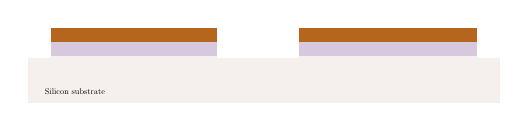
\begin{tikzpicture}[node distance = 3cm, auto, thick,scale=\CrossSectionOnly, every node/.style={transform shape}]
		% substrate
\fill[substrate] (0,0) rectangle (20,1.9);
\node at (2,0.5) {Silicon substrate};

% substrate islands
\fill[substrate] (1,1.9) rectangle (8,2);
\fill[substrate] (11.5,1.9) rectangle (19,2);

% pad oxide
\fill[isolationoxide] (1,2) rectangle (8,2.6);
\fill[isolationoxide] (11.5,2) rectangle (19,2.6);

% resist
\fill[resist] (1,2.6) rectangle (8,3.2);
\fill[resist] (11.5,2.6) rectangle (19,3.2);
	\end{tikzpicture} \\
	
\includegraphics[scale=0.01]{down_arrow.png} \\
	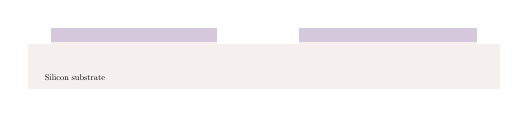
\begin{tikzpicture}[node distance = 3cm, auto, thick,scale=\CrossSectionOnly, every node/.style={transform shape}]
		% substrate
\fill[substrate] (0,0) rectangle (20,1.9);
\node at (2,0.5) {Silicon substrate};

% substrate islands
\fill[substrate] (1,1.9) rectangle (8,2);
\fill[substrate] (11.5,1.9) rectangle (19,2);

% pad oxide
\fill[isolationoxide] (1,2) rectangle (8,2.6);
\fill[isolationoxide] (11.5,2) rectangle (19,2.6);
	\end{tikzpicture}
	\caption{Resist removal}
\end{figure}

We strip the resist, rinse and perform sulfuric cleaning.

\newpage

\subsection{Silicon etching}\label{sti_trench_etch}

Silicon can only be etched by a very aggressive chemical cocktail of  KOH and TMAH (20\%) or by plasma etching.

\begin{figure}[H]
	\centering
	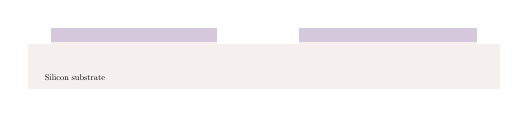
\begin{tikzpicture}[node distance = 3cm, auto, thick,scale=\CrossSectionOnly, every node/.style={transform shape}]
		% substrate
\fill[substrate] (0,0) rectangle (20,1.9);
\node at (2,0.5) {Silicon substrate};

% substrate islands
\fill[substrate] (1,1.9) rectangle (8,2);
\fill[substrate] (11.5,1.9) rectangle (19,2);

% pad oxide
\fill[isolationoxide] (1,2) rectangle (8,2.6);
\fill[isolationoxide] (11.5,2) rectangle (19,2.6);
	\end{tikzpicture} \\
	
\includegraphics[scale=0.01]{down_arrow.png} \\
	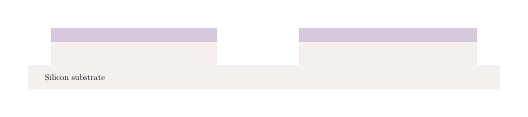
\begin{tikzpicture}[node distance = 3cm, auto, thick,scale=\CrossSectionOnly, every node/.style={transform shape}]
		% substrate
\fill[substrate] (0,0) rectangle (20,1);
\node at (2,0.5) {Silicon substrate};

% substrate islands
\fill[substrate] (1,1) rectangle (8,2);
\fill[substrate] (11.5,1) rectangle (19,2);

% pad oxide
\fill[isolationoxide] (1,2) rectangle (8,2.6);
\fill[isolationoxide] (11.5,2) rectangle (19,2.6);
	\end{tikzpicture}
	\caption{Trench etching}
\end{figure}

\textbf{Possible approaches}:
\begin{itemize}
\item \textbf{"DRIE Etcher \#1" from HKUST} \\
Has a normal etching rate of up to $2\frac{\mu m}{min}$.
This means we etch for 10 minutes with a reduced etch speed of $200\frac{nm}{min}$ in order to be clearly deep enough and to compensate for different etch depths in different places.
This way we have a good chance of having proper isolation everywhere on the wafer.

\item \textbf{Chemical solution} \\
Using a KOH solution of 20\% at 60\degreesC gives us an etch rate of roughly  26.57\um per hour\footnote{\url{http://www.lelandstanfordjunior.com/KOH.html}}.
\begin{itemize}
\item The <100> etch rate is: 26.57 micron/hr = 0.44 micron/min
\item The <110> etch rate is: 40.5 micron/hr 
\item The <111> etch rate is: 0.4932 micron/hr 
\item The SiO2 etch rate is: 49.92 nanometers/hr 
\end{itemize}
With a desired depth of 2\um we will have to etch around 4 minutes and 30 seconds in order to reach the desired depth.
The disadvantage of this approach is the imprecision and under-etch of the mask.
\end{itemize}

\subsection{Hard mask: Removal}

Now we have to remove the oxide hard mask for further processing in order to proceed with well formation without contamination during oxide growing.

\begin{figure}[H]
	\centering
	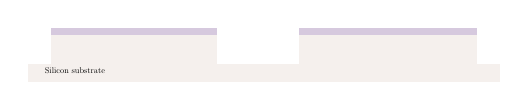
\begin{tikzpicture}[node distance = 3cm, auto, thick,scale=\CrossSectionOnly, every node/.style={transform shape}]
		% substrate
\fill[substrate] (0,0) rectangle (20,0.75);
\node at (2,0.5) {Silicon substrate};

% substrate islands
\fill[substrate] (1,0.75) rectangle (8,2);
\fill[substrate] (11.5,0.75) rectangle (19,2);

% covering oxide
\fill[isolationoxide] (1,2) rectangle (8,2.3);
\fill[isolationoxide] (11.5,2) rectangle (19,2.3);
	\end{tikzpicture} \\
	
\includegraphics[scale=0.01]{down_arrow.png} \\
	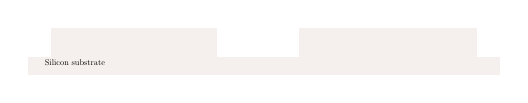
\begin{tikzpicture}[node distance = 3cm, auto, thick,scale=\CrossSectionOnly, every node/.style={transform shape}]
		% substrate
\fill[substrate] (0,0) rectangle (20,0.75);
\node at (2,0.5) {Silicon substrate};

% substrate islands
\fill[substrate] (1,0.75) rectangle (8,2);
\fill[substrate] (11.5,0.75) rectangle (19,2);
	\end{tikzpicture}
	\caption{Trench etching}
\end{figure}

We use buffered hydrofluoric acid (BOE (1:6)) at room temperature for a little bit over 3 minutes in order to remove all of the 300nm thick oxide layer.
\newpage
\subsection{Well}\label{well}
In order to build CMOS on the same substrate, an n-well is required for building the complementary P-channel transistor for a n-p-channel logic circuitry as shown above in the example section.
The cross section as well as the top view of the targeted geometry are shown in \autoref{nwell_target}
\begin{figure}[H]
	\centering
	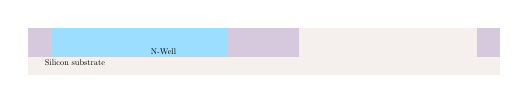
\begin{tikzpicture}[node distance = 3cm, auto, thick,scale=\CrossAndTopSectionBig, every node/.style={transform shape}]
		% substrate
\fill[substrate] (0,0) rectangle (20,2);
\node at (2,0.5) {Silicon substrate};
%trenches
\fill[isolationoxide] (0,0.75) rectangle (1,2);
\fill[isolationoxide] (8.5,0.75) rectangle (11.5,2);
\fill[isolationoxide] (19,0.75) rectangle (20,2);
% n-well
\fill[nwell] (1,0.75) rectangle (8.5,2);
\node at (5.75,1) {N-Well};
	\end{tikzpicture}
	
\begin{tikzpicture}[node distance = 3cm, auto, thick,scale=\CrossAndTopSectionBig, every node/.style={transform shape}]
		% substrate
\fill[YellowOrange] (0,0) rectangle (20,12);
% n-well
\fill[Goldenrod] (1.25,1.5) rectangle (8.25,7.25);
	\end{tikzpicture}
	\caption{N-well target geometry}
	\label{nwell_target}
\end{figure}
The n-well will serve us as an island of n-doped substrate within the p-doped basis substrate.
the n-well forms a natural p-n-junction to the later on implanted channel-stop which has a nice side effect of being an additional polarity protection.
The dopant dose will be: $2.5\times10^{12}cm^{-2}$

The surface concentration of the n-well ($\approx 1 \times 10^{16} cm^{-3}$) is determined primarily by the need to maintain a sufficient high surface concentration to prevent field inversion of the n-well.
The depth of the n-well ($\approx 4 \mu m$) is then determined by the need to prevent punch-through of the parasitic vertical pnp transistor under worst case bias conditions.

\begin{figure}[H]
	\centering
	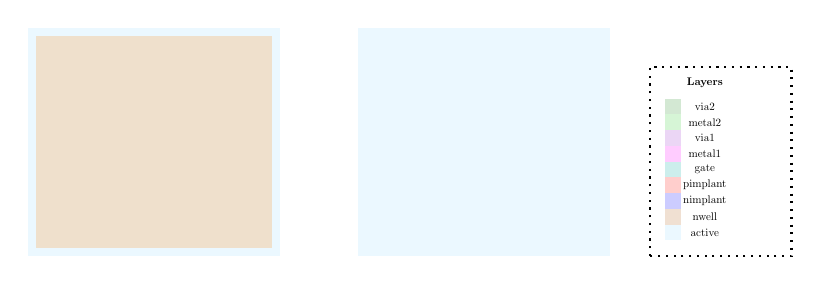
\begin{tikzpicture}[node distance = 3cm, auto, thick,scale=\VLSILayout, every node/.style={transform shape}]
		\fill[nwell,opacity=0.2] (0.75,0.5) rectangle (8.75,7.75);
\fill[nwell,opacity=0.2] (11.25,0.5) rectangle (19.25,7.75);

\draw[dotted] (20.5,0.5) rectangle (25,6.5);

\node at (22.25,6) {\textbf{Layers}};

\fill[nwell,opacity=0.2] (21,1) rectangle (21.5,1.5);
\node at (22.25,1.25) {active};

\fill[resist,opacity=0.2] (21,1.5) rectangle (21.5,2);
\node at (22.25,1.75) {nwell};

\fill[blue,opacity=0.2] (21,2) rectangle (21.5,2.5);
\node at (22.25,2.25) {nimplant};

\fill[nitride,opacity=0.2] (21,2.5) rectangle (21.5,3);
\node at (22.25,2.75) {pimplant};

\fill[Emerald,opacity=0.2] (21,3) rectangle (21.5,3.5);
\node at (22.25,3.25) {gate};

\fill[Fuchsia,opacity=0.2] (21,3.5) rectangle (21.5,4);
\node at (22.25,3.75) {metal1};

\fill[DarkOrchid,opacity=0.2] (21,4) rectangle (21.5,4.5);
\node at (22.25,4.25) {via1};

\fill[LimeGreen,opacity=0.2] (21,4.5) rectangle (21.5,5);
\node at (22.25,4.75) {metal2};

\fill[ForestGreen,opacity=0.2] (21,5) rectangle (21.5,5.5);
\node at (22.25,5.25) {via2};

\fill[orange,opacity=0.2] (1,0.75) rectangle (8.5,7.5);
	\end{tikzpicture}
	\caption{N-Well layout}
	\label{well_layout}
\end{figure}

In \autoref{well_layout} the layout of the n-well region on top of the active area region can be seen.
You should make the active area always a little bit bigger than the n-well area in order to avoid hitting parts of the trench oxide with your dopant.

\newpage

\subsubsection{Mask dioxide layer}
In order to selectively inject charge carrying atoms into the crystalline structure a protective dioxide ($SiO_2$) layer needs to be grown on top of a p-type substrate.
\begin{figure}[H]
	\centering
	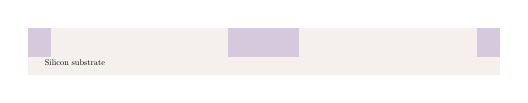
\begin{tikzpicture}[node distance = 3cm, auto, thick,scale=\CrossSectionOnly, every node/.style={transform shape}]
		% substrate
\fill[substrate] (0,0) rectangle (20,2);
\node at (2,0.5) {Silicon substrate};
%trenches
\fill[isolationoxide] (0,0.75) rectangle (1,2);
\fill[isolationoxide] (8.5,0.75) rectangle (11.5,2);
\fill[isolationoxide] (19,0.75) rectangle (20,2);
	\end{tikzpicture} \\
	
\includegraphics[scale=0.01]{down_arrow.png} \\
	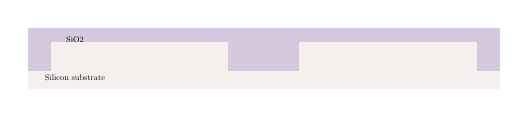
\begin{tikzpicture}[node distance = 3cm, auto, thick,scale=\CrossSectionOnly, every node/.style={transform shape}]
		% substrate
\fill[substrate] (0,0) rectangle (20,2);
\node at (2,0.5) {Silicon substrate};
%trenches
\fill[isolationoxide] (0,0.75) rectangle (1,2);
\fill[isolationoxide] (8.5,0.75) rectangle (11.5,2);
\fill[isolationoxide] (19,0.75) rectangle (20,2);
% oxide
\fill[isolationoxide] (0,2) rectangle (20,2.6);
\node at (2,2.1) {SiO2};
	\end{tikzpicture}
	\caption{Dioxide layer growth}
\end{figure}
The industrial best practice is a layer of around (500nm$\approx$5000\normalfont\AA) thickness or more.
For this purpose the wafer is being oxidized for at least 90 minutes at 1000\degree C using wet oxidation which results in a dioxide layer at least 500nm($\approx$5000\normalfont\AA) in thickness.

\subsubsection{Patterning}
The resist is being deposited using spin coating and then baked depending on the baking time for the specific resist.
The layout for being exposed onto the resist is being extracted from the "nwell" layer within the GDS2 file.
\begin{figure}[H]
	\centering
	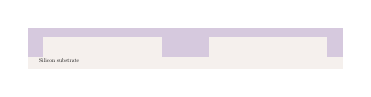
\begin{tikzpicture}[node distance = 3cm, auto, thick,scale=\CrossAndTopSection, every node/.style={transform shape}]
		% substrate
\fill[substrate] (0,0) rectangle (20,2);
\node at (2,0.5) {Silicon substrate};
%trenches
\fill[isolationoxide] (0,0.75) rectangle (1,2);
\fill[isolationoxide] (8.5,0.75) rectangle (11.5,2);
\fill[isolationoxide] (19,0.75) rectangle (20,2);
% oxide
\fill[isolationoxide] (0,2) rectangle (20,2.6);
	\end{tikzpicture}
	
\begin{tikzpicture}[node distance = 3cm, auto, thick,scale=\CrossAndTopSection, every node/.style={transform shape}]
		% resist
\fill[gray] (0,0) rectangle (20,12);
	\end{tikzpicture} \\
	
\includegraphics[scale=0.01]{down_arrow.png} \\
	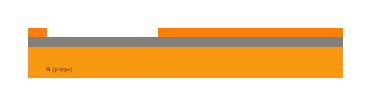
\begin{tikzpicture}[node distance = 3cm, auto, thick,scale=\CrossAndTopSection, every node/.style={transform shape}]
		% substrate
\fill[YellowOrange] (0,0) rectangle (20,2);
\node at (2,0.5) {Si (p-type)};
% oxide
\fill[gray] (0,2) rectangle (20,2.6);
% resist
\fill[orange] (0,2.6) rectangle (1.25,3.2);
\fill[orange] (8.25,2.6) rectangle (20,3.2);
	\end{tikzpicture}
	
\begin{tikzpicture}[node distance = 3cm, auto, thick,scale=\CrossAndTopSection, every node/.style={transform shape}]
		% resist
\fill[resist] (0,0) rectangle (20,12);
% substrate
\fill[isolationoxide] (1.25,1.5) rectangle (8.25,7.25);
	\end{tikzpicture}
	\caption{Cross/top view of n-well layout on resist}
\end{figure}
The thickness of the resist layer and the baking duration will variate depending on the specific equipment for which this process will be implemented with.

\subsubsection{Etching}
We now need to open a window in the dioxide layer, through which we will inject carrier atoms into the silicon crystal structure.
\begin{figure}[H]
	\centering
	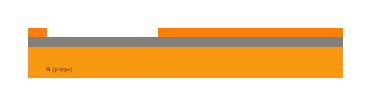
\begin{tikzpicture}[node distance = 3cm, auto, thick,scale=\CrossAndTopSection, every node/.style={transform shape}]
		% substrate
\fill[YellowOrange] (0,0) rectangle (20,2);
\node at (2,0.5) {Si (p-type)};
% oxide
\fill[gray] (0,2) rectangle (20,2.6);
% resist
\fill[orange] (0,2.6) rectangle (1.25,3.2);
\fill[orange] (8.25,2.6) rectangle (20,3.2);
	\end{tikzpicture}
	
\begin{tikzpicture}[node distance = 3cm, auto, thick,scale=\CrossAndTopSection, every node/.style={transform shape}]
		% resist
\fill[resist] (0,0) rectangle (20,12);
% substrate
\fill[isolationoxide] (1.25,1.5) rectangle (8.25,7.25);
	\end{tikzpicture} \\
	
\includegraphics[scale=0.01]{down_arrow.png} \\
	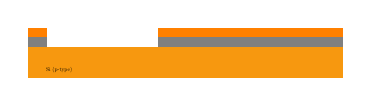
\begin{tikzpicture}[node distance = 3cm, auto, thick,scale=\CrossAndTopSection, every node/.style={transform shape}]
		% substrate
\fill[YellowOrange] (0,0) rectangle (20,2);
\node at (2,0.5) {Si (p-type)};
% oxide
\fill[gray] (0,2) rectangle (1.25,2.6);
\fill[gray] (8.25,2) rectangle (20,2.6);
% resist
\fill[orange] (0,2.6) rectangle (1.25,3.2);
\fill[orange] (8.25,2.6) rectangle (20,3.2);
	\end{tikzpicture}
	
\begin{tikzpicture}[node distance = 3cm, auto, thick,scale=\CrossAndTopSection, every node/.style={transform shape}]
		% resist
\fill[orange] (0,0) rectangle (20,12);
% substrate
\fill[YellowOrange] (1.25,1.5) rectangle (8.25,7.25);
	\end{tikzpicture}
	\caption{Cross/top view of n-well oxide window}
\end{figure}
Since the silicon dioxide layer is 500nm thick and we wanna reach the silicon below we can use wet etching as described in the chemistry chapter.
Using BHF (6:1) (\autoref{BHF_six_to_one}) we can etch with a speed of approximately 2 nm/s at 25 \degree C, we can calculate the etching time to be $\frac{500nm}{2nm/s}$=250s=4 minutes 10 seconds (or make it rather 30 seconds instead of 10)

\subsubsection{Cleaning}
In order to avoid contamination of the machines we need to make sure all the resist has been stripped off from the wafer.
\begin{figure}[H]
	\centering
	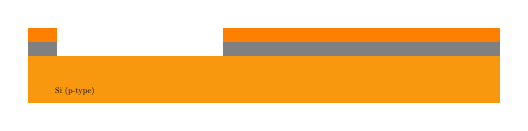
\begin{tikzpicture}[node distance = 3cm, auto, thick,scale=\CrossSectionOnly, every node/.style={transform shape}]
		% substrate
\fill[YellowOrange] (0,0) rectangle (20,2);
\node at (2,0.5) {Si (p-type)};
% oxide
\fill[gray] (0,2) rectangle (1.25,2.6);
\fill[gray] (8.25,2) rectangle (20,2.6);
% resist
\fill[orange] (0,2.6) rectangle (1.25,3.2);
\fill[orange] (8.25,2.6) rectangle (20,3.2);
	\end{tikzpicture} \\
	
\includegraphics[scale=0.01]{down_arrow.png} \\
	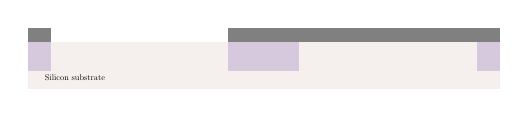
\begin{tikzpicture}[node distance = 3cm, auto, thick,scale=\CrossSectionOnly, every node/.style={transform shape}]
		% substrate
\fill[substrate] (0,0) rectangle (20,2);
\node at (2,0.5) {Silicon substrate};
%trenches
\fill[isolationoxide] (0,0.75) rectangle (1,2);
\fill[isolationoxide] (8.5,0.75) rectangle (11.5,2);
\fill[isolationoxide] (19,0.75) rectangle (20,2);
% oxide
\fill[gray] (0,2) rectangle (1,2.6);
\fill[gray] (8.5,2) rectangle (20,2.6);
	\end{tikzpicture}
	\caption{Resist removal}
\end{figure}
Please just use the solvent for the specific resist.

\subsubsection{Injection}
We now need to inject the carriers into the upper level of the n-channel area so that we can later on drive them into the crystal during the drive-in step.
\begin{figure}[H]
	\centering
	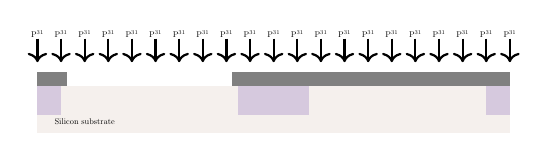
\begin{tikzpicture}[node distance = 3cm, auto, thick,scale=\CrossSectionOnly, every node/.style={transform shape}]
		% substrate
\fill[substrate] (0,0) rectangle (20,2);
\node at (2,0.5) {Silicon substrate};
%trenches
\fill[isolationoxide] (0,0.75) rectangle (1,2);
\fill[isolationoxide] (8.5,0.75) rectangle (11.5,2);
\fill[isolationoxide] (19,0.75) rectangle (20,2);
% oxide
\fill[gray] (0,2) rectangle (1.25,2.6);
\fill[gray] (8.25,2) rectangle (20,2.6);

\forloop{ct}{0}{\value{ct} < 21}
{
	\draw [->] (\value{ct},4) -- (\value{ct},3);
	\node at (\value{ct},4.2) {P$^{31}$};
}
	\end{tikzpicture} \\
	
\includegraphics[scale=0.01]{down_arrow.png} \\
	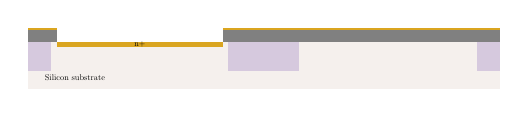
\begin{tikzpicture}[node distance = 3cm, auto, thick,scale=\CrossSectionOnly, every node/.style={transform shape}]
		% substrate
\fill[substrate] (0,0) rectangle (20,2);
\node at (2,0.5) {Silicon substrate};
%trenches
\fill[isolationoxide] (0,0.75) rectangle (1,2);
\fill[isolationoxide] (8.5,0.75) rectangle (11.5,2);
\fill[isolationoxide] (19,0.75) rectangle (20,2);
% phosphorus
\fill[Goldenrod] (1.25,1.8) rectangle (8.25,2);
\node at (4.75,1.9) {n+};
% oxide
\fill[gray] (0,2) rectangle (1.25,2.6);
\fill[gray] (8.25,2) rectangle (20,2.6);
\fill[Goldenrod] (0,2.5) rectangle (1.25,2.6);
\fill[Goldenrod] (8.25,2.5) rectangle (20,2.6);
	\end{tikzpicture}
	\caption{Doping process}
\end{figure}
The n-well is implanted with a Phosphorus ($P^{31}$) dose of $2.5\times10^{12}cm^{-2}$ at an energy of 100 KeV.
The n-well is then annealed.

\subsubsection{Oxide for drive-in}
Now we need to cover the now doped and annealed areas with an oxide layer for the drive-in phase.
\begin{figure}[H]
	\centering
	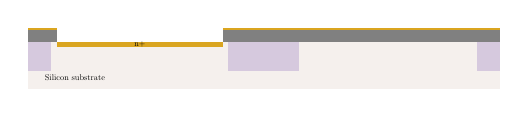
\begin{tikzpicture}[node distance = 3cm, auto, thick,scale=\CrossSectionOnly, every node/.style={transform shape}]
		% substrate
\fill[substrate] (0,0) rectangle (20,2);
\node at (2,0.5) {Silicon substrate};
%trenches
\fill[isolationoxide] (0,0.75) rectangle (1,2);
\fill[isolationoxide] (8.5,0.75) rectangle (11.5,2);
\fill[isolationoxide] (19,0.75) rectangle (20,2);
% phosphorus
\fill[Goldenrod] (1.25,1.8) rectangle (8.25,2);
\node at (4.75,1.9) {n+};
% oxide
\fill[gray] (0,2) rectangle (1.25,2.6);
\fill[gray] (8.25,2) rectangle (20,2.6);
\fill[Goldenrod] (0,2.5) rectangle (1.25,2.6);
\fill[Goldenrod] (8.25,2.5) rectangle (20,2.6);
	\end{tikzpicture} \\
	
\includegraphics[scale=0.01]{down_arrow.png} \\
	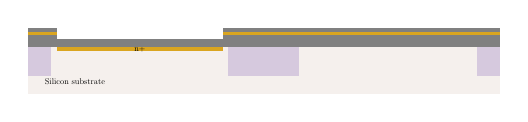
\begin{tikzpicture}[node distance = 3cm, auto, thick,scale=\CrossSectionOnly, every node/.style={transform shape}]
		% substrate
\fill[substrate] (0,0) rectangle (20,2);
\node at (2,0.5) {Silicon substrate};
%trenches
\fill[isolationoxide] (0,0.75) rectangle (1,2);
\fill[isolationoxide] (8.5,0.75) rectangle (11.5,2);
\fill[isolationoxide] (19,0.75) rectangle (20,2);
% phosphorus
\fill[Goldenrod] (1.25,1.8) rectangle (8.25,2.0);
\node at (4.75,1.9) {n+};
% oxide
\fill[gray] (0,2) rectangle (1.25,2.8);
\fill[gray] (1.25,2) rectangle (8.25,2.3);
\fill[gray] (8.25,2) rectangle (20,2.8);
\fill[Goldenrod] (0,2.5) rectangle (1.25,2.6);
\fill[Goldenrod] (8.25,2.5) rectangle (20,2.6);
	\end{tikzpicture}
	\caption{Oxide growth}
\end{figure}
The wafer is being oxidized for 32 minutes at 1000\degree C in order to achieve a cover silicon layer of 250nm thickness ($\approx$2500\normalfont\AA).

\subsubsection{Drive-in}
In order to drive the carrier atoms deeper into the crystalline structure the wafer needs to be driven in after predeposition.
\begin{figure}[H]
	\centering
	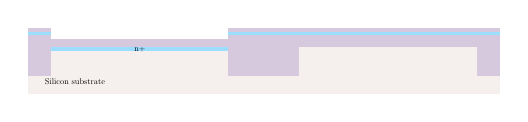
\begin{tikzpicture}[node distance = 3cm, auto, thick,scale=\CrossSectionOnly, every node/.style={transform shape}]
		% substrate
\fill[substrate] (0,0) rectangle (20,2);
\node at (2,0.5) {Silicon substrate};
%trenches
\fill[isolationoxide] (0,0.75) rectangle (1,2);
\fill[isolationoxide] (8.5,0.75) rectangle (11.5,2);
\fill[isolationoxide] (19,0.75) rectangle (20,2);
% phosphorus
\fill[nwell] (1,1.8) rectangle (8.5,2.0);
\node at (4.75,1.9) {n+};

% oxide
\fill[isolationoxide] (0,2) rectangle (1,2.8);
\fill[isolationoxide] (1,2) rectangle (8.5,2.3);
\fill[isolationoxide] (8.5,2) rectangle (20,2.8);
		
\fill[nwell] (0,2.5) rectangle (1,2.6);
\fill[nwell] (8.5,2.5) rectangle (20,2.6);
	\end{tikzpicture} \\
	
\includegraphics[scale=0.01]{down_arrow.png} \\
	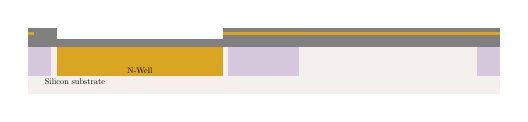
\begin{tikzpicture}[node distance = 3cm, auto, thick,scale=\CrossSectionOnly, every node/.style={transform shape}]
		% substrate
\fill[substrate] (0,0) rectangle (20,2);
\node at (2,0.5) {Silicon substrate};
%trenches
\fill[isolationoxide] (0,0.75) rectangle (1,2);
\fill[isolationoxide] (8.5,0.75) rectangle (11.5,2);
\fill[isolationoxide] (19,0.75) rectangle (20,2);
% n-well
\fill[Goldenrod] (1.25,0.75) rectangle (8.25,2);
\node at (4.75,1) {N-Well};
% oxide
\fill[gray] (0,2) rectangle (1.25,2.8);
\fill[gray] (1.25,2) rectangle (8.25,2.3);
\fill[gray] (8.25,2) rectangle (20,2.8);
		
\fill[Goldenrod] (0,2.5) rectangle (0.25,2.6);
\fill[Goldenrod] (8.25,2.5) rectangle (20,2.6);
	\end{tikzpicture}
	\caption{Drive-in process}
\end{figure}
In this step the wafer is  driven-in for 960 minutes at 1150\degree C in an inert ambient.

\subsubsection{Oxide mask removal}
We want to remove the silicon mask from the wafer so that the n-well becomes accessible for the further process steps but we don't want to etch "way too much" of the trench material.
\begin{figure}[H]
	\centering
	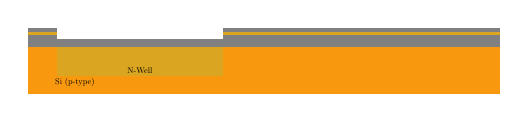
\begin{tikzpicture}[node distance = 3cm, auto, thick,scale=\CrossSectionOnly, every node/.style={transform shape}]
		% substrate
\fill[YellowOrange] (0,0) rectangle (20,2);
\node at (2,0.5) {Si (p-type)};
% n-well
\fill[Goldenrod] (1.25,0.75) rectangle (8.25,2);
\node at (4.75,1) {N-Well};
% oxide
\fill[gray] (0,2) rectangle (1.25,2.8);
\fill[gray] (1.25,2) rectangle (8.25,2.3);
\fill[gray] (8.25,2) rectangle (20,2.8);
\fill[Goldenrod] (0,2.5) rectangle (1.25,2.6);
\fill[Goldenrod] (8.25,2.5) rectangle (20,2.6);
	\end{tikzpicture} \\
	
\includegraphics[scale=0.01]{down_arrow.png} \\
	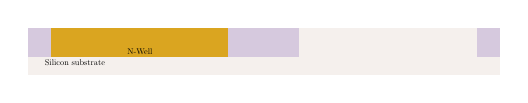
\begin{tikzpicture}[node distance = 3cm, auto, thick,scale=\CrossSectionOnly, every node/.style={transform shape}]
		% substrate
\fill[substrate] (0,0) rectangle (20,2);
\node at (2,0.5) {Silicon substrate};
%trenches
\fill[isolationoxide] (0,0.75) rectangle (1,2);
\fill[isolationoxide] (8.5,0.75) rectangle (11.5,2);
\fill[isolationoxide] (19,0.75) rectangle (20,2);

% n-well
\fill[Goldenrod] (1,0.75) rectangle (8.5,2);
\node at (4.75,1) {N-Well};
	\end{tikzpicture}
	\caption{Oxide removal}
\end{figure}
Since the silicon dioxide layer is 750nm (500nm+250nm) thick and we wanna reach the silicon below we can use wet etching as described in the chemistry chapter.
Using BHF (6:1) (\autoref{BHF_six_to_one}) we can etch with a speed of approximately 2 nm/s at 25 \degree C.
We can calculate the etching time to be $\frac{750nm}{2nm/s}$=375s=6 Minutes and 15 Seconds.

Etching away a "little bit too much" of the oxide isn't that bad, because the oxide within the trenches will be "filled up" again during the later steps.

\newpage
\subsection{n+ Implant}
\begin{center}
	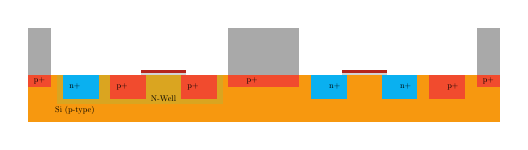
\begin{tikzpicture}[node distance = 3cm, auto, thick,scale=0.3, every node/.style={transform shape}]
		% substrate
		\fill[YellowOrange] (0,0) rectangle (20,2);
		\node at (2,0.5) {Si (p-type)};
		% n-well
		\fill[Goldenrod] (1.25,0.75) rectangle (8.25,2);
		\node at (5.75,1) {N-Well};
		% body
		\fill[ProcessBlue] (1.5,1) rectangle (3,2);
		\node at (2,1.5) {n+};
		% source
		\fill[RedOrange] (3.5,1) rectangle (5,2);
		\node at (4,1.5) {p+};
		% drain
		\fill[RedOrange] (6.5,1) rectangle (8,2);
		\node at (7,1.5) {p+};
		%% gate:
		% gate oxide
		\fill[LightGray] (4.8,2) rectangle (6.7,2.1);
		% gate poly
		\fill[BrickRed] (4.8,2.1) rectangle (6.7,2.2);

		%field oxides:
		\fill[DarkGray] (0,2) rectangle (1,4);
		\fill[DarkGray] (8.5,2) rectangle (11.5,4);
		\fill[DarkGray] (19,2) rectangle (20,4);

		\fill[RedOrange] (0,1.5) rectangle (1,2);
		\fill[RedOrange] (8.5,1.5) rectangle (11.5,2);
		\fill[RedOrange] (19,1.5) rectangle (20,2);

		\node at (0.5,1.75) {p+};
		\node at (9.5,1.75) {p+};
		\node at (19.5,1.75) {p+};

		%%% nmos:
		% body
		\fill[RedOrange] (17,1) rectangle (18.5,2);
		\node at (18,1.5) {p+};
		% source
		\fill[ProcessBlue] (15,1) rectangle (16.5,2);
		\node at (16,1.5) {n+};
		% drain
		\fill[ProcessBlue] (12,1) rectangle (13.5,2);
		\node at (13,1.5) {n+};

		%% gate:
		% gate oxide
		\fill[LightGray] (13.3,2) rectangle (15.2,2.1);
		% gate poly
		\fill[BrickRed] (13.3,2.1) rectangle (15.2,2.2);
	\end{tikzpicture}
	
\begin{tikzpicture}[node distance = 3cm, auto, thick,scale=0.3, every node/.style={transform shape}]
		\fill[YellowOrange] (0,0) rectangle (20,10);
		% n-well
		\fill[Goldenrod] (1.25,1.5) rectangle (8.25,7.25);
		% p+
		\fill[RedOrange] (3.5,2) rectangle (5,6.5);
		\fill[RedOrange] (6.5,2) rectangle (8,6.5);
		\fill[RedOrange] (17,2) rectangle (18.5,6.5);
		% n+
		\fill[ProcessBlue] (1.5,2) rectangle (3,6.5);
		\fill[ProcessBlue] (12,2) rectangle (13.5,6.5);
		\fill[ProcessBlue] (15,2) rectangle (16.5,6.5);
		% field oxide
		\fill[DarkGray] (0,0) rectangle (1,12);
		\fill[DarkGray] (8.5,0) rectangle (11.5,12);
		\fill[DarkGray] (19,0) rectangle (20,12);
		\fill[DarkGray] (0,0) rectangle (20,1.25);
		\fill[DarkGray] (0,7.5) rectangle (20,12);
		% poly
		\fill[BrickRed] (4.8,1.75) rectangle (6.7,9);
		\fill[BrickRed] (13.3,1.75) rectangle (15.2,9);
		\fill[BrickRed] (4.8,8) rectangle (15.2,9);
	\end{tikzpicture}
\end{center}

\subsubsection{Pattering}
\begin{center}
	\begin{tikzpicture}[node distance = 3cm, auto, thick,scale=0.2, every node/.style={transform shape}]
		% substrate
		\fill[YellowOrange] (0,0) rectangle (20,2);
		\node at (2,0.5) {Si (p-type)};
		% n-well
		\fill[Goldenrod] (1.25,0.75) rectangle (8.25,2);
		\node at (4.75,1) {N-Well};
		% gate oxide
		\fill[LightGray] (4.8,2) rectangle (6.7,2.1);
		\fill[LightGray] (13.3,2) rectangle (15.2,2.1);
		% gate poly
		\fill[BrickRed] (4.8,2.1) rectangle (6.7,2.2);
		\fill[BrickRed] (13.3,2.1) rectangle (15.2,2.2);
		% dioxide
		\fill[NormalGray] (0,2) rectangle (3.5,2.7);
		\fill[NormalGray] (8,2) rectangle (13.3,2.7);
		\fill[NormalGray] (13.3,2.2) rectangle (15.2,2.7);
		\fill[NormalGray] (15.2,2) rectangle (17,2.7);
		\fill[NormalGray] (18.5,2) rectangle (20,2.7);
		% dioxide 2nd
		\fill[NormalGray] (0,2.8) rectangle (3.5,3.3);
		\fill[NormalGray] (3.5,2) rectangle (4.8,2.8);
		\fill[NormalGray] (4.8,2.3) rectangle (6.7,2.8);
		\fill[NormalGray] (6.7,2) rectangle (8,2.8);
		\fill[NormalGray] (8,2.8) rectangle (8.5,3.3);
		\fill[NormalGray] (11.5,2.8) rectangle (17,3.3);
		\fill[NormalGray] (17,2) rectangle (18.5,2.8);
		\fill[NormalGray] (18.5,2.8) rectangle (19,3.3);
		\fill[DarkGray] (0,4.1) rectangle (1,4.2);
		\fill[DarkGray] (8.5,4.1) rectangle (11.5,4.2);
		\fill[DarkGray] (19,4.1) rectangle (20,4.2);
		% p+
		\fill[RedOrange] (0,4) rectangle (1,4.1);
		\fill[RedOrange] (1,2.7) rectangle (3.5,2.8);
		\fill[RedOrange] (8,2.7) rectangle (8.5,2.8);
		\fill[RedOrange] (8.5,4) rectangle (11.5,4.1);
		\fill[RedOrange] (11.5,2.7) rectangle (17,2.8);
		\fill[RedOrange] (18.5,2.7) rectangle (19,2.8);
		\fill[RedOrange] (19,4) rectangle (20,4.1);
		\fill[RedOrange] (3.4,1.2) rectangle (4.9,2);
		\fill[RedOrange] (4.8,2.2) rectangle (6.7,2.3);
		\fill[RedOrange] (6.6,1.2) rectangle (8.1,2);
		\fill[RedOrange] (16.9,1.2) rectangle (18.7,2);
		%field oxides:
		\fill[DarkGray] (0,2) rectangle (1,4);
		\fill[DarkGray] (8.5,2) rectangle (11.5,4);
		\fill[DarkGray] (19,2) rectangle (20,4);
		% channel stop
		\fill[RedOrange] (0,1.5) rectangle (1,2);
		\fill[RedOrange] (8.5,1.5) rectangle (11.5,2);
		\fill[RedOrange] (19,1.5) rectangle (20,2);
	\end{tikzpicture}
	\begin{tikzpicture}[node distance = 3cm, auto, thick,scale=0.2, every node/.style={transform shape}]
		\fill[DarkGray] (0,0) rectangle (20,12);
		\fill[NormalGray] (1,1.25) rectangle (8.5,7.5);
		\fill[NormalGray] (11.5,1.25) rectangle (19,7.5);
	\end{tikzpicture}

	
\includegraphics[scale=0.01]{down_arrow.png}

	\begin{tikzpicture}[node distance = 3cm, auto, thick,scale=0.2, every node/.style={transform shape}]
		% substrate
		\fill[YellowOrange] (0,0) rectangle (20,2);
		\node at (2,0.5) {Si (p-type)};
		% n-well
		\fill[Goldenrod] (1.25,0.75) rectangle (8.25,2);
		\node at (4.75,1) {N-Well};
		% gate oxide
		\fill[LightGray] (4.8,2) rectangle (6.7,2.1);
		\fill[LightGray] (13.3,2) rectangle (15.2,2.1);
		% gate poly
		\fill[BrickRed] (4.8,2.1) rectangle (6.7,2.2);
		\fill[BrickRed] (13.3,2.1) rectangle (15.2,2.2);
		% dioxide
		\fill[NormalGray] (0,2) rectangle (3.5,2.7);
		\fill[NormalGray] (8,2) rectangle (13.3,2.7);
		\fill[NormalGray] (13.3,2.2) rectangle (15.2,2.7);
		\fill[NormalGray] (15.2,2) rectangle (17,2.7);
		\fill[NormalGray] (18.5,2) rectangle (20,2.7);
		% dioxide 2nd
		\fill[NormalGray] (0,2.8) rectangle (3.5,3.3);
		\fill[NormalGray] (3.5,2) rectangle (4.8,2.8);
		\fill[NormalGray] (4.8,2.3) rectangle (6.7,2.8);
		\fill[NormalGray] (6.7,2) rectangle (8,2.8);
		\fill[NormalGray] (8,2.8) rectangle (8.5,3.3);
		\fill[NormalGray] (11.5,2.8) rectangle (17,3.3);
		\fill[NormalGray] (17,2) rectangle (18.5,2.8);
		\fill[NormalGray] (18.5,2.8) rectangle (19,3.3);
		\fill[NormalGray] (0,4.1) rectangle (1,4.2);
		\fill[NormalGray] (8.5,4.1) rectangle (11.5,4.2);
		\fill[NormalGray] (19,4.1) rectangle (20,4.2);
		% resist
		\fill[orange] (0,3.3) rectangle (1.6,4.8);
		\fill[orange] (2.9,3.3) rectangle (3.5,4.8);
		\fill[orange] (3.5,2.8) rectangle (4.8,4.8);
		\fill[orange] (4.8,2.8) rectangle (6.7,4.8);
		\fill[orange] (6.7,2.8) rectangle (8,4.8);
		\fill[orange] (8,3.3) rectangle (8.5,4.8);
		\fill[orange] (11.5,3.3) rectangle (12,4.8);
		\fill[orange] (16.5,3.3) rectangle (17,4.8);
		\fill[orange] (17,2.8) rectangle (18.5,4.8);
		\fill[orange] (18.5,3.3) rectangle (19,4.8);
		\fill[orange] (0,4.2) rectangle (1,4.8);
		\fill[orange] (8.5,4.2) rectangle (11.5,4.8);
		\fill[orange] (19,4.2) rectangle (20,4.8);
		% p+
		\fill[RedOrange] (0,4) rectangle (1,4.1);
		\fill[RedOrange] (1,2.7) rectangle (3.5,2.8);
		\fill[RedOrange] (8,2.7) rectangle (8.5,2.8);
		\fill[RedOrange] (8.5,4) rectangle (11.5,4.1);
		\fill[RedOrange] (11.5,2.7) rectangle (17,2.8);
		\fill[RedOrange] (18.5,2.7) rectangle (19,2.8);
		\fill[RedOrange] (19,4) rectangle (20,4.1);
		\fill[RedOrange] (3.4,1.2) rectangle (4.9,2);
		\fill[RedOrange] (4.8,2.2) rectangle (6.7,2.3);
		\fill[RedOrange] (6.6,1.2) rectangle (8.1,2);
		\fill[RedOrange] (16.9,1.2) rectangle (18.7,2);
		%field oxides:
		\fill[DarkGray] (0,2) rectangle (1,4);
		\fill[DarkGray] (8.5,2) rectangle (11.5,4);
		\fill[DarkGray] (19,2) rectangle (20,4);
		% channel stop
		\fill[RedOrange] (0,1.5) rectangle (1,2);
		\fill[RedOrange] (8.5,1.5) rectangle (11.5,2);
		\fill[RedOrange] (19,1.5) rectangle (20,2);
	\end{tikzpicture}
	\begin{tikzpicture}[node distance = 3cm, auto, thick,scale=0.2, every node/.style={transform shape}]
		\fill[orange] (0,0) rectangle (20,12);
		% n+
		\fill[NormalGray] (1.5,2) rectangle (3,6.5);
		\fill[NormalGray] (12,2) rectangle (16.5,6.5);
	\end{tikzpicture}
\end{center}

\subsubsection{Etching}
\begin{center}
	\begin{tikzpicture}[node distance = 3cm, auto, thick,scale=0.2, every node/.style={transform shape}]
		% substrate
		\fill[YellowOrange] (0,0) rectangle (20,2);
		\node at (2,0.5) {Si (p-type)};
		% n-well
		\fill[Goldenrod] (1.25,0.75) rectangle (8.25,2);
		\node at (4.75,1) {N-Well};
		% gate oxide
		\fill[LightGray] (4.8,2) rectangle (6.7,2.1);
		\fill[LightGray] (13.3,2) rectangle (15.2,2.1);
		% gate poly
		\fill[BrickRed] (4.8,2.1) rectangle (6.7,2.2);
		\fill[BrickRed] (13.3,2.1) rectangle (15.2,2.2);
		% dioxide
		\fill[NormalGray] (0,2) rectangle (3.5,2.7);
		\fill[NormalGray] (8,2) rectangle (13.3,2.7);
		\fill[NormalGray] (13.3,2.2) rectangle (15.2,2.7);
		\fill[NormalGray] (15.2,2) rectangle (17,2.7);
		\fill[NormalGray] (18.5,2) rectangle (20,2.7);
		% dioxide 2nd
		\fill[NormalGray] (0,2.8) rectangle (3.5,3.3);
		\fill[NormalGray] (3.5,2) rectangle (4.8,2.8);
		\fill[NormalGray] (4.8,2.3) rectangle (6.7,2.8);
		\fill[NormalGray] (6.7,2) rectangle (8,2.8);
		\fill[NormalGray] (8,2.8) rectangle (8.5,3.3);
		\fill[NormalGray] (11.5,2.8) rectangle (17,3.3);
		\fill[NormalGray] (17,2) rectangle (18.5,2.8);
		\fill[NormalGray] (18.5,2.8) rectangle (19,3.3);
		\fill[NormalGray] (0,4.1) rectangle (1,4.2);
		\fill[NormalGray] (8.5,4.1) rectangle (11.5,4.2);
		\fill[NormalGray] (19,4.1) rectangle (20,4.2);
		% resist
		\fill[orange] (0,3.3) rectangle (1.6,4.8);
		\fill[orange] (2.9,3.3) rectangle (3.5,4.8);
		\fill[orange] (3.5,2.8) rectangle (4.8,4.8);
		\fill[orange] (4.8,2.8) rectangle (6.7,4.8);
		\fill[orange] (6.7,2.8) rectangle (8,4.8);
		\fill[orange] (8,3.3) rectangle (8.5,4.8);
		\fill[orange] (11.5,3.3) rectangle (12,4.8);
		\fill[orange] (16.5,3.3) rectangle (17,4.8);
		\fill[orange] (17,2.8) rectangle (18.5,4.8);
		\fill[orange] (18.5,3.3) rectangle (19,4.8);
		\fill[orange] (0,4.2) rectangle (1,4.8);
		\fill[orange] (8.5,4.2) rectangle (11.5,4.8);
		\fill[orange] (19,4.2) rectangle (20,4.8);
		% p+
		\fill[RedOrange] (0,4) rectangle (1,4.1);
		\fill[RedOrange] (1,2.7) rectangle (3.5,2.8);
		\fill[RedOrange] (8,2.7) rectangle (8.5,2.8);
		\fill[RedOrange] (8.5,4) rectangle (11.5,4.1);
		\fill[RedOrange] (11.5,2.7) rectangle (17,2.8);
		\fill[RedOrange] (18.5,2.7) rectangle (19,2.8);
		\fill[RedOrange] (19,4) rectangle (20,4.1);
		\fill[RedOrange] (3.4,1.2) rectangle (4.9,2);
		\fill[RedOrange] (4.8,2.2) rectangle (6.7,2.3);
		\fill[RedOrange] (6.6,1.2) rectangle (8.1,2);
		\fill[RedOrange] (16.9,1.2) rectangle (18.7,2);
		%field oxides:
		\fill[DarkGray] (0,2) rectangle (1,4);
		\fill[DarkGray] (8.5,2) rectangle (11.5,4);
		\fill[DarkGray] (19,2) rectangle (20,4);
		% channel stop
		\fill[RedOrange] (0,1.5) rectangle (1,2);
		\fill[RedOrange] (8.5,1.5) rectangle (11.5,2);
		\fill[RedOrange] (19,1.5) rectangle (20,2);
	\end{tikzpicture}
	\begin{tikzpicture}[node distance = 3cm, auto, thick,scale=0.2, every node/.style={transform shape}]
		\fill[orange] (0,0) rectangle (20,12);
		% n+
		\fill[NormalGray] (1.5,2) rectangle (3,6.5);
		\fill[NormalGray] (12,2) rectangle (16.5,6.5);
	\end{tikzpicture}
	
	
\includegraphics[scale=0.01]{down_arrow.png}

	\begin{tikzpicture}[node distance = 3cm, auto, thick,scale=0.2, every node/.style={transform shape}]
		% substrate
		\fill[YellowOrange] (0,0) rectangle (20,2);
		\node at (2,0.5) {Si (p-type)};
		% n-well
		\fill[Goldenrod] (1.25,0.75) rectangle (8.25,2);
		\node at (4.75,1) {N-Well};
		% gate oxide
		\fill[LightGray] (4.8,2) rectangle (6.7,2.1);
		\fill[LightGray] (13.3,2) rectangle (15.2,2.1);
		% gate poly
		\fill[BrickRed] (4.8,2.1) rectangle (6.7,2.2);
		\fill[BrickRed] (13.3,2.1) rectangle (15.2,2.2);
		% dioxide
		\fill[NormalGray] (1,2) rectangle (1.6,2.7); % fox
		\fill[NormalGray] (2.9,2) rectangle (3.5,2.7); % fox
		\fill[NormalGray] (8,2) rectangle (8.5,2.7);
		\fill[NormalGray] (11,2) rectangle (12,2.7); % fox
		\fill[NormalGray] (16.5,2) rectangle (17,2.7); % fox
		\fill[NormalGray] (18.5,2) rectangle (20,2.7);
		% dioxide 2nd
		\fill[NormalGray] (1,2.8) rectangle (1.6,3.3); % fox
		\fill[NormalGray] (2.9,2.8) rectangle (3.5,3.3); % fox
		\fill[NormalGray] (3.5,2) rectangle (4.8,2.8);
		\fill[NormalGray] (4.8,2.3) rectangle (6.7,2.8);
		\fill[NormalGray] (6.7,2) rectangle (8,2.8);
		\fill[NormalGray] (8,2.8) rectangle (8.5,3.3);
		\fill[NormalGray] (11.5,2.8) rectangle (12,3.3); % fox
		\fill[NormalGray] (16.5,2.8) rectangle (17,3.3); % fox
		\fill[NormalGray] (17,2) rectangle (18.5,2.8);
		\fill[NormalGray] (18.5,2.8) rectangle (19,3.3);
		\fill[NormalGray] (0,4.1) rectangle (1,4.2);
		\fill[NormalGray] (8.5,4.1) rectangle (11.5,4.2);
		\fill[NormalGray] (19,4.1) rectangle (20,4.2);
		% resist
		\fill[orange] (0,3.3) rectangle (1.6,4.8);
		\fill[orange] (2.9,3.3) rectangle (3.5,4.8);
		\fill[orange] (3.5,2.8) rectangle (4.8,4.8);
		\fill[orange] (4.8,2.8) rectangle (6.7,4.8);
		\fill[orange] (6.7,2.8) rectangle (8,4.8);
		\fill[orange] (8,3.3) rectangle (8.5,4.8);
		\fill[orange] (11.5,3.3) rectangle (12,4.8);
		\fill[orange] (16.5,3.3) rectangle (17,4.8);
		\fill[orange] (17,2.8) rectangle (18.5,4.8);
		\fill[orange] (18.5,3.3) rectangle (19,4.8);
		\fill[orange] (0,4.2) rectangle (1,4.8);
		\fill[orange] (8.5,4.2) rectangle (11.5,4.8);
		\fill[orange] (19,4.2) rectangle (20,4.8);
		% p+
		\fill[RedOrange] (0,4) rectangle (1,4.1);
		\fill[RedOrange] (1,2.7) rectangle (1.6,2.8);
		\fill[RedOrange] (2.9,2.7) rectangle (3.5,2.8);
		\fill[RedOrange] (8,2.7) rectangle (8.5,2.8);
		\fill[RedOrange] (8.5,4) rectangle (11.5,4.1);
		\fill[RedOrange] (11.5,2.7) rectangle (12,2.8); % fox
		\fill[RedOrange] (16.5,2.7) rectangle (17,2.8); % fox
		\fill[RedOrange] (18.5,2.7) rectangle (19,2.8);
		\fill[RedOrange] (19,4) rectangle (20,4.1);
		\fill[RedOrange] (3.4,1.2) rectangle (4.9,2);
		\fill[RedOrange] (4.8,2.2) rectangle (6.7,2.3);
		\fill[RedOrange] (6.6,1.2) rectangle (8.1,2);
		\fill[RedOrange] (16.9,1.2) rectangle (18.7,2);
		%field oxides:
		\fill[DarkGray] (0,2) rectangle (1,4);
		\fill[DarkGray] (8.5,2) rectangle (11.5,4);
		\fill[DarkGray] (19,2) rectangle (20,4);
		% channel stop
		\fill[RedOrange] (0,1.5) rectangle (1,2);
		\fill[RedOrange] (8.5,1.5) rectangle (11.5,2);
		\fill[RedOrange] (19,1.5) rectangle (20,2);
	\end{tikzpicture}
	\begin{tikzpicture}[node distance = 3cm, auto, thick,scale=0.2, every node/.style={transform shape}]
		\fill[orange] (0,0) rectangle (20,12);
		\fill[Goldenrod] (1.5,2) rectangle (3,6.5);
		\fill[YellowOrange] (12,2) rectangle (16.5,6.5);
		\fill[BrickRed] (13.3,2) rectangle (15.2,6.5);
	\end{tikzpicture}
\end{center}

\subsubsection{Cleaning}
\begin{center}
	\begin{tikzpicture}[node distance = 3cm, auto, thick,scale=0.2, every node/.style={transform shape}]
		% substrate
		\fill[YellowOrange] (0,0) rectangle (20,2);
		\node at (2,0.5) {Si (p-type)};
		% n-well
		\fill[Goldenrod] (1.25,0.75) rectangle (8.25,2);
		\node at (4.75,1) {N-Well};
		% gate oxide
		\fill[LightGray] (4.8,2) rectangle (6.7,2.1);
		\fill[LightGray] (13.3,2) rectangle (15.2,2.1);
		% gate poly
		\fill[BrickRed] (4.8,2.1) rectangle (6.7,2.2);
		\fill[BrickRed] (13.3,2.1) rectangle (15.2,2.2);
		% dioxide
		\fill[NormalGray] (1,2) rectangle (1.6,2.7); % fox
		\fill[NormalGray] (2.9,2) rectangle (3.5,2.7); % fox
		\fill[NormalGray] (8,2) rectangle (8.5,2.7);
		\fill[NormalGray] (11,2) rectangle (12,2.7); % fox
		\fill[NormalGray] (16.5,2) rectangle (17,2.7); % fox
		\fill[NormalGray] (18.5,2) rectangle (20,2.7);
		% dioxide 2nd
		\fill[NormalGray] (1,2.8) rectangle (1.6,3.3); % fox
		\fill[NormalGray] (2.9,2.8) rectangle (3.5,3.3); % fox
		\fill[NormalGray] (3.5,2) rectangle (4.8,2.8);
		\fill[NormalGray] (4.8,2.3) rectangle (6.7,2.8);
		\fill[NormalGray] (6.7,2) rectangle (8,2.8);
		\fill[NormalGray] (8,2.8) rectangle (8.5,3.3);
		\fill[NormalGray] (11.5,2.8) rectangle (12,3.3); % fox
		\fill[NormalGray] (16.5,2.8) rectangle (17,3.3); % fox
		\fill[NormalGray] (17,2) rectangle (18.5,2.8);
		\fill[NormalGray] (18.5,2.8) rectangle (19,3.3);
		\fill[NormalGray] (0,4.1) rectangle (1,4.2);
		\fill[NormalGray] (8.5,4.1) rectangle (11.5,4.2);
		\fill[NormalGray] (19,4.1) rectangle (20,4.2);
		% resist
		\fill[orange] (0,3.3) rectangle (1.6,4.8);
		\fill[orange] (2.9,3.3) rectangle (3.5,4.8);
		\fill[orange] (3.5,2.8) rectangle (4.8,4.8);
		\fill[orange] (4.8,2.8) rectangle (6.7,4.8);
		\fill[orange] (6.7,2.8) rectangle (8,4.8);
		\fill[orange] (8,3.3) rectangle (8.5,4.8);
		\fill[orange] (11.5,3.3) rectangle (12,4.8);
		\fill[orange] (16.5,3.3) rectangle (17,4.8);
		\fill[orange] (17,2.8) rectangle (18.5,4.8);
		\fill[orange] (18.5,3.3) rectangle (19,4.8);
		\fill[orange] (0,4.2) rectangle (1,4.8);
		\fill[orange] (8.5,4.2) rectangle (11.5,4.8);
		\fill[orange] (19,4.2) rectangle (20,4.8);
		% p+
		\fill[RedOrange] (0,4) rectangle (1,4.1);
		\fill[RedOrange] (1,2.7) rectangle (1.6,2.8);
		\fill[RedOrange] (2.9,2.7) rectangle (3.5,2.8);
		\fill[RedOrange] (8,2.7) rectangle (8.5,2.8);
		\fill[RedOrange] (8.5,4) rectangle (11.5,4.1);
		\fill[RedOrange] (11.5,2.7) rectangle (12,2.8); % fox
		\fill[RedOrange] (16.5,2.7) rectangle (17,2.8); % fox
		\fill[RedOrange] (18.5,2.7) rectangle (19,2.8);
		\fill[RedOrange] (19,4) rectangle (20,4.1);
		\fill[RedOrange] (3.4,1.2) rectangle (4.9,2);
		\fill[RedOrange] (4.8,2.2) rectangle (6.7,2.3);
		\fill[RedOrange] (6.6,1.2) rectangle (8.1,2);
		\fill[RedOrange] (16.9,1.2) rectangle (18.7,2);
		%field oxides:
		\fill[DarkGray] (0,2) rectangle (1,4);
		\fill[DarkGray] (8.5,2) rectangle (11.5,4);
		\fill[DarkGray] (19,2) rectangle (20,4);
		% channel stop
		\fill[RedOrange] (0,1.5) rectangle (1,2);
		\fill[RedOrange] (8.5,1.5) rectangle (11.5,2);
		\fill[RedOrange] (19,1.5) rectangle (20,2);
	\end{tikzpicture}
	\begin{tikzpicture}[node distance = 3cm, auto, thick,scale=0.2, every node/.style={transform shape}]
		\fill[orange] (0,0) rectangle (20,12);
		\fill[Goldenrod] (1.5,2) rectangle (3,6.5);
		\fill[YellowOrange] (12,2) rectangle (16.5,6.5);
		\fill[BrickRed] (13.3,2) rectangle (15.2,6.5);
	\end{tikzpicture}

	
\includegraphics[scale=0.01]{down_arrow.png}

	\begin{tikzpicture}[node distance = 3cm, auto, thick,scale=0.2, every node/.style={transform shape}]
		% substrate
		\fill[YellowOrange] (0,0) rectangle (20,2);
		\node at (2,0.5) {Si (p-type)};
		% n-well
		\fill[Goldenrod] (1.25,0.75) rectangle (8.25,2);
		\node at (4.75,1) {N-Well};
		% gate oxide
		\fill[LightGray] (4.8,2) rectangle (6.7,2.1);
		\fill[LightGray] (13.3,2) rectangle (15.2,2.1);
		% gate poly
		\fill[BrickRed] (4.8,2.1) rectangle (6.7,2.2);
		\fill[BrickRed] (13.3,2.1) rectangle (15.2,2.2);
		% dioxide
		\fill[NormalGray] (1,2) rectangle (1.6,2.7); % fox
		\fill[NormalGray] (2.9,2) rectangle (3.5,2.7); % fox
		\fill[NormalGray] (8,2) rectangle (8.5,2.7);
		\fill[NormalGray] (11,2) rectangle (12,2.7); % fox
		\fill[NormalGray] (16.5,2) rectangle (17,2.7); % fox
		\fill[NormalGray] (18.5,2) rectangle (20,2.7);
		% dioxide 2nd
		\fill[NormalGray] (1,2.8) rectangle (1.6,3.3); % fox
		\fill[NormalGray] (2.9,2.8) rectangle (3.5,3.3); % fox
		\fill[NormalGray] (3.5,2) rectangle (4.8,2.8);
		\fill[NormalGray] (4.8,2.3) rectangle (6.7,2.8);
		\fill[NormalGray] (6.7,2) rectangle (8,2.8);
		\fill[NormalGray] (8,2.8) rectangle (8.5,3.3);
		\fill[NormalGray] (11.5,2.8) rectangle (12,3.3); % fox
		\fill[NormalGray] (16.5,2.8) rectangle (17,3.3); % fox
		\fill[NormalGray] (17,2) rectangle (18.5,2.8);
		\fill[NormalGray] (18.5,2.8) rectangle (19,3.3);
		\fill[NormalGray] (0,4.1) rectangle (1,4.2);
		\fill[NormalGray] (8.5,4.1) rectangle (11.5,4.2);
		\fill[NormalGray] (19,4.1) rectangle (20,4.2);
		% p+
		\fill[RedOrange] (0,4) rectangle (1,4.1);
		\fill[RedOrange] (1,2.7) rectangle (1.6,2.8);
		\fill[RedOrange] (2.9,2.7) rectangle (3.5,2.8);
		\fill[RedOrange] (8,2.7) rectangle (8.5,2.8);
		\fill[RedOrange] (8.5,4) rectangle (11.5,4.1);
		\fill[RedOrange] (11.5,2.7) rectangle (12,2.8); % fox
		\fill[RedOrange] (16.5,2.7) rectangle (17,2.8); % fox
		\fill[RedOrange] (18.5,2.7) rectangle (19,2.8);
		\fill[RedOrange] (19,4) rectangle (20,4.1);
		\fill[RedOrange] (3.4,1.2) rectangle (4.9,2);
		\fill[RedOrange] (4.8,2.2) rectangle (6.7,2.3);
		\fill[RedOrange] (6.6,1.2) rectangle (8.1,2);
		\fill[RedOrange] (16.9,1.2) rectangle (18.7,2);
		%field oxides:
		\fill[DarkGray] (0,2) rectangle (1,4);
		\fill[DarkGray] (8.5,2) rectangle (11.5,4);
		\fill[DarkGray] (19,2) rectangle (20,4);
		% channel stop
		\fill[RedOrange] (0,1.5) rectangle (1,2);
		\fill[RedOrange] (8.5,1.5) rectangle (11.5,2);
		\fill[RedOrange] (19,1.5) rectangle (20,2);
	\end{tikzpicture}
	\begin{tikzpicture}[node distance = 3cm, auto, thick,scale=0.2, every node/.style={transform shape}]
		\fill[DarkGray] (0,0) rectangle (20,12);
		\fill[NormalGray] (1,1.25) rectangle (8.5,7.5);
		\fill[NormalGray] (11.5,1.25) rectangle (19,7.5);
		\fill[Goldenrod] (1.5,2) rectangle (3,6.5);
		\fill[YellowOrange] (12,2) rectangle (16.5,6.5);
		\fill[BrickRed] (13.3,2) rectangle (15.2,6.5);
	\end{tikzpicture}
\end{center}

\subsubsection{Predeposition}
\begin{center}
	\begin{tikzpicture}[node distance = 3cm, auto, thick,scale=0.3, every node/.style={transform shape}]
		% substrate
		\fill[YellowOrange] (0,0) rectangle (20,2);
		\node at (2,0.5) {Si (p-type)};
		% n-well
		\fill[Goldenrod] (1.25,0.75) rectangle (8.25,2);
		\node at (4.75,1) {N-Well};
		% gate oxide
		\fill[LightGray] (4.8,2) rectangle (6.7,2.1);
		\fill[LightGray] (13.3,2) rectangle (15.2,2.1);
		% gate poly
		\fill[BrickRed] (4.8,2.1) rectangle (6.7,2.2);
		\fill[BrickRed] (13.3,2.1) rectangle (15.2,2.2);
		% dioxide
		\fill[NormalGray] (1,2) rectangle (1.6,2.7); % fox
		\fill[NormalGray] (2.9,2) rectangle (3.5,2.7); % fox
		\fill[NormalGray] (8,2) rectangle (8.5,2.7);
		\fill[NormalGray] (11,2) rectangle (12,2.7); % fox
		\fill[NormalGray] (16.5,2) rectangle (17,2.7); % fox
		\fill[NormalGray] (18.5,2) rectangle (20,2.7);
		% dioxide 2nd
		\fill[NormalGray] (1,2.8) rectangle (1.6,3.3); % fox
		\fill[NormalGray] (2.9,2.8) rectangle (3.5,3.3); % fox
		\fill[NormalGray] (3.5,2) rectangle (4.8,2.8);
		\fill[NormalGray] (4.8,2.3) rectangle (6.7,2.8);
		\fill[NormalGray] (6.7,2) rectangle (8,2.8);
		\fill[NormalGray] (8,2.8) rectangle (8.5,3.3);
		\fill[NormalGray] (11.5,2.8) rectangle (12,3.3); % fox
		\fill[NormalGray] (16.5,2.8) rectangle (17,3.3); % fox
		\fill[NormalGray] (17,2) rectangle (18.5,2.8);
		\fill[NormalGray] (18.5,2.8) rectangle (19,3.3);
		\fill[NormalGray] (0,4.1) rectangle (1,4.2);
		\fill[NormalGray] (8.5,4.1) rectangle (11.5,4.2);
		\fill[NormalGray] (19,4.1) rectangle (20,4.2);
		% p+
		\fill[RedOrange] (0,4) rectangle (1,4.1);
		\fill[RedOrange] (1,2.7) rectangle (1.6,2.8);
		\fill[RedOrange] (2.9,2.7) rectangle (3.5,2.8);
		\fill[RedOrange] (8,2.7) rectangle (8.5,2.8);
		\fill[RedOrange] (8.5,4) rectangle (11.5,4.1);
		\fill[RedOrange] (11.5,2.7) rectangle (12,2.8); % fox
		\fill[RedOrange] (16.5,2.7) rectangle (17,2.8); % fox
		\fill[RedOrange] (18.5,2.7) rectangle (19,2.8);
		\fill[RedOrange] (19,4) rectangle (20,4.1);
		\fill[RedOrange] (3.4,1.2) rectangle (4.9,2);
		\fill[RedOrange] (4.8,2.2) rectangle (6.7,2.3);
		\fill[RedOrange] (6.6,1.2) rectangle (8.1,2);
		\fill[RedOrange] (16.9,1.2) rectangle (18.7,2);
		%field oxides:
		\fill[DarkGray] (0,2) rectangle (1,4);
		\fill[DarkGray] (8.5,2) rectangle (11.5,4);
		\fill[DarkGray] (19,2) rectangle (20,4);
		% channel stop
		\fill[RedOrange] (0,1.5) rectangle (1,2);
		\fill[RedOrange] (8.5,1.5) rectangle (11.5,2);
		\fill[RedOrange] (19,1.5) rectangle (20,2);

		\forloop{ct}{0}{\value{ct} < 21}
		{
			\draw [->] (\value{ct},5) -- (\value{ct},4.2);
			\node at (\value{ct},5.2) {P$^{31}$};
		}
	\end{tikzpicture}

	
\includegraphics[scale=0.01]{down_arrow.png}

	\begin{tikzpicture}[node distance = 3cm, auto, thick,scale=0.3, every node/.style={transform shape}]
		% substrate
		\fill[YellowOrange] (0,0) rectangle (20,2);
		\node at (2,0.5) {Si (p-type)};
		% n-well
		\fill[Goldenrod] (1.25,0.75) rectangle (8.25,2);
		\node at (4.75,1) {N-Well};
		% gate oxide
		\fill[LightGray] (4.8,2) rectangle (6.7,2.1);
		\fill[LightGray] (13.3,2) rectangle (15.2,2.1);
		% gate poly
		\fill[BrickRed] (4.8,2.1) rectangle (6.7,2.2);
		\fill[BrickRed] (13.3,2.1) rectangle (15.2,2.2);
		% dioxide
		\fill[NormalGray] (1,2) rectangle (1.6,2.7); % fox
		\fill[NormalGray] (2.9,2) rectangle (3.5,2.7); % fox
		\fill[NormalGray] (8,2) rectangle (8.5,2.7);
		\fill[NormalGray] (11,2) rectangle (12,2.7); % fox
		\fill[NormalGray] (16.5,2) rectangle (17,2.7); % fox
		\fill[NormalGray] (18.5,2) rectangle (20,2.7);
		% dioxide 2nd
		\fill[NormalGray] (1,2.8) rectangle (1.6,3.3); % fox
		\fill[NormalGray] (2.9,2.8) rectangle (3.5,3.3); % fox
		\fill[NormalGray] (3.5,2) rectangle (4.8,2.8);
		\fill[NormalGray] (4.8,2.3) rectangle (6.7,2.8);
		\fill[NormalGray] (6.7,2) rectangle (8,2.8);
		\fill[NormalGray] (8,2.8) rectangle (8.5,3.3);
		\fill[NormalGray] (11.5,2.8) rectangle (12,3.3); % fox
		\fill[NormalGray] (16.5,2.8) rectangle (17,3.3); % fox
		\fill[NormalGray] (17,2) rectangle (18.5,2.8);
		\fill[NormalGray] (18.5,2.8) rectangle (19,3.3);
		\fill[NormalGray] (0,4.1) rectangle (1,4.2);
		\fill[NormalGray] (8.5,4.1) rectangle (11.5,4.2);
		\fill[NormalGray] (19,4.1) rectangle (20,4.2);
		% p+
		\fill[RedOrange] (0,4) rectangle (1,4.1);
		\fill[RedOrange] (1,2.7) rectangle (1.6,2.8);
		\fill[RedOrange] (2.9,2.7) rectangle (3.5,2.8);
		\fill[RedOrange] (8,2.7) rectangle (8.5,2.8);
		\fill[RedOrange] (8.5,4) rectangle (11.5,4.1);
		\fill[RedOrange] (11.5,2.7) rectangle (12,2.8); % fox
		\fill[RedOrange] (16.5,2.7) rectangle (17,2.8); % fox
		\fill[RedOrange] (18.5,2.7) rectangle (19,2.8);
		\fill[RedOrange] (19,4) rectangle (20,4.1);
		\fill[RedOrange] (3.4,1.2) rectangle (4.9,2);
		\fill[RedOrange] (4.8,2.2) rectangle (6.7,2.3);
		\fill[RedOrange] (6.6,1.2) rectangle (8.1,2);
		\fill[RedOrange] (16.9,1.2) rectangle (18.7,2);
		% n+
		\fill[ProcessBlue] (1.6,1.8) rectangle (2.9,2);
		\fill[ProcessBlue] (12,1.8) rectangle (13.3,2);
		\fill[ProcessBlue] (15.2,1.8) rectangle (16.5,2);
		% n+ on oxide
		\fill[ProcessBlue] (0,4.2) rectangle (1,4.3);
		\fill[ProcessBlue] (1,3.3) rectangle (1.6,3.4);
		\fill[ProcessBlue] (2.9,3.3) rectangle (3.5,3.4);
		\fill[ProcessBlue] (3.5,2.8) rectangle (8,2.9);
		\fill[ProcessBlue] (8,3.3) rectangle (8.5,3.4);
		\fill[ProcessBlue] (8.5,4.2) rectangle (11.5,4.3);
		\fill[ProcessBlue] (11.5,3.3) rectangle (12,3.4);
		\fill[ProcessBlue] (13.3,2.2) rectangle (15.2,2.3);
		\fill[ProcessBlue] (16.5,3.3) rectangle (17,3.4);
		\fill[ProcessBlue] (17,2.8) rectangle (18.5,2.9);
		\fill[ProcessBlue] (18.5,3.3) rectangle (19,3.4);
		\fill[ProcessBlue] (19,4.2) rectangle (20,4.3);
		%field oxides:
		\fill[DarkGray] (0,2) rectangle (1,4);
		\fill[DarkGray] (8.5,2) rectangle (11.5,4);
		\fill[DarkGray] (19,2) rectangle (20,4);
		% channel stop
		\fill[RedOrange] (0,1.5) rectangle (1,2);
		\fill[RedOrange] (8.5,1.5) rectangle (11.5,2);
		\fill[RedOrange] (19,1.5) rectangle (20,2);
	\end{tikzpicture}
\end{center}

\subsubsection{Sacrificial oxide}
\begin{center}
	\begin{tikzpicture}[node distance = 3cm, auto, thick,scale=0.3, every node/.style={transform shape}]
		% substrate
		\fill[YellowOrange] (0,0) rectangle (20,2);
		\node at (2,0.5) {Si (p-type)};
		% n-well
		\fill[Goldenrod] (1.25,0.75) rectangle (8.25,2);
		\node at (4.75,1) {N-Well};
		% gate oxide
		\fill[LightGray] (4.8,2) rectangle (6.7,2.1);
		\fill[LightGray] (13.3,2) rectangle (15.2,2.1);
		% gate poly
		\fill[BrickRed] (4.8,2.1) rectangle (6.7,2.2);
		\fill[BrickRed] (13.3,2.1) rectangle (15.2,2.2);
		% dioxide
		\fill[NormalGray] (1,2) rectangle (1.6,2.7); % fox
		\fill[NormalGray] (2.9,2) rectangle (3.5,2.7); % fox
		\fill[NormalGray] (8,2) rectangle (8.5,2.7);
		\fill[NormalGray] (11,2) rectangle (12,2.7); % fox
		\fill[NormalGray] (16.5,2) rectangle (17,2.7); % fox
		\fill[NormalGray] (18.5,2) rectangle (20,2.7);
		% dioxide 2nd
		\fill[NormalGray] (1,2.8) rectangle (1.6,3.3); % fox
		\fill[NormalGray] (2.9,2.8) rectangle (3.5,3.3); % fox
		\fill[NormalGray] (3.5,2) rectangle (4.8,2.8);
		\fill[NormalGray] (4.8,2.3) rectangle (6.7,2.8);
		\fill[NormalGray] (6.7,2) rectangle (8,2.8);
		\fill[NormalGray] (8,2.8) rectangle (8.5,3.3);
		\fill[NormalGray] (11.5,2.8) rectangle (12,3.3); % fox
		\fill[NormalGray] (16.5,2.8) rectangle (17,3.3); % fox
		\fill[NormalGray] (17,2) rectangle (18.5,2.8);
		\fill[NormalGray] (18.5,2.8) rectangle (19,3.3);
		\fill[NormalGray] (0,4.1) rectangle (1,4.2);
		\fill[NormalGray] (8.5,4.1) rectangle (11.5,4.2);
		\fill[NormalGray] (19,4.1) rectangle (20,4.2);
		% p+
		\fill[RedOrange] (0,4) rectangle (1,4.1);
		\fill[RedOrange] (1,2.7) rectangle (1.6,2.8);
		\fill[RedOrange] (2.9,2.7) rectangle (3.5,2.8);
		\fill[RedOrange] (8,2.7) rectangle (8.5,2.8);
		\fill[RedOrange] (8.5,4) rectangle (11.5,4.1);
		\fill[RedOrange] (11.5,2.7) rectangle (12,2.8); % fox
		\fill[RedOrange] (16.5,2.7) rectangle (17,2.8); % fox
		\fill[RedOrange] (18.5,2.7) rectangle (19,2.8);
		\fill[RedOrange] (19,4) rectangle (20,4.1);
		\fill[RedOrange] (3.4,1.2) rectangle (4.9,2);
		\fill[RedOrange] (4.8,2.2) rectangle (6.7,2.3);
		\fill[RedOrange] (6.6,1.2) rectangle (8.1,2);
		\fill[RedOrange] (16.9,1.2) rectangle (18.7,2);
		% n+
		\fill[ProcessBlue] (1.6,1.8) rectangle (2.9,2);
		\fill[ProcessBlue] (12,1.8) rectangle (13.3,2);
		\fill[ProcessBlue] (15.2,1.8) rectangle (16.5,2);
		% n+ on oxide
		\fill[ProcessBlue] (0,4.2) rectangle (1,4.3);
		\fill[ProcessBlue] (1,3.3) rectangle (1.6,3.4);
		\fill[ProcessBlue] (2.9,3.3) rectangle (3.5,3.4);
		\fill[ProcessBlue] (3.5,2.8) rectangle (8,2.9);
		\fill[ProcessBlue] (8,3.3) rectangle (8.5,3.4);
		\fill[ProcessBlue] (8.5,4.2) rectangle (11.5,4.3);
		\fill[ProcessBlue] (11.5,3.3) rectangle (12,3.4);
		\fill[ProcessBlue] (13.3,2.2) rectangle (15.2,2.3);
		\fill[ProcessBlue] (16.5,3.3) rectangle (17,3.4);
		\fill[ProcessBlue] (17,2.8) rectangle (18.5,2.9);
		\fill[ProcessBlue] (18.5,3.3) rectangle (19,3.4);
		\fill[ProcessBlue] (19,4.2) rectangle (20,4.3);
		%field oxides:
		\fill[DarkGray] (0,2) rectangle (1,4);
		\fill[DarkGray] (8.5,2) rectangle (11.5,4);
		\fill[DarkGray] (19,2) rectangle (20,4);
		% channel stop
		\fill[RedOrange] (0,1.5) rectangle (1,2);
		\fill[RedOrange] (8.5,1.5) rectangle (11.5,2);
		\fill[RedOrange] (19,1.5) rectangle (20,2);
	\end{tikzpicture}

	
\includegraphics[scale=0.01]{down_arrow.png}

	\begin{tikzpicture}[node distance = 3cm, auto, thick,scale=0.3, every node/.style={transform shape}]
		% substrate
		\fill[YellowOrange] (0,0) rectangle (20,2);
		\node at (2,0.5) {Si (p-type)};
		% n-well
		\fill[Goldenrod] (1.25,0.75) rectangle (8.25,2);
		\node at (4.75,1) {N-Well};
		% gate oxide
		\fill[LightGray] (4.8,2) rectangle (6.7,2.1);
		\fill[LightGray] (13.3,2) rectangle (15.2,2.1);
		% gate poly
		\fill[BrickRed] (4.8,2.1) rectangle (6.7,2.2);
		\fill[BrickRed] (13.3,2.1) rectangle (15.2,2.2);
		% dioxide
		\fill[NormalGray] (1,2) rectangle (1.6,2.7); % fox
		\fill[NormalGray] (2.9,2) rectangle (3.5,2.7); % fox
		\fill[NormalGray] (8,2) rectangle (8.5,2.7);
		\fill[NormalGray] (11,2) rectangle (12,2.7); % fox
		\fill[NormalGray] (16.5,2) rectangle (17,2.7); % fox
		\fill[NormalGray] (18.5,2) rectangle (20,2.7);
		% dioxide 2nd
		\fill[NormalGray] (1,2.8) rectangle (1.6,3.3); % fox
		\fill[NormalGray] (2.9,2.8) rectangle (3.5,3.3); % fox
		\fill[NormalGray] (3.5,2) rectangle (4.8,2.8);
		\fill[NormalGray] (4.8,2.3) rectangle (6.7,2.8);
		\fill[NormalGray] (6.7,2) rectangle (8,2.8);
		\fill[NormalGray] (8,2.8) rectangle (8.5,3.3);
		\fill[NormalGray] (11.5,2.8) rectangle (12,3.3); % fox
		\fill[NormalGray] (16.5,2.8) rectangle (17,3.3); % fox
		\fill[NormalGray] (17,2) rectangle (18.5,2.8);
		\fill[NormalGray] (18.5,2.8) rectangle (19,3.3);
		\fill[NormalGray] (0,4.1) rectangle (1,4.2);
		\fill[NormalGray] (8.5,4.1) rectangle (11.5,4.2);
		\fill[NormalGray] (19,4.1) rectangle (20,4.2);
		% p+
		\fill[RedOrange] (0,4) rectangle (1,4.1);
		\fill[RedOrange] (1,2.7) rectangle (1.6,2.8);
		\fill[RedOrange] (2.9,2.7) rectangle (3.5,2.8);
		\fill[RedOrange] (8,2.7) rectangle (8.5,2.8);
		\fill[RedOrange] (8.5,4) rectangle (11.5,4.1);
		\fill[RedOrange] (11.5,2.7) rectangle (12,2.8); % fox
		\fill[RedOrange] (16.5,2.7) rectangle (17,2.8); % fox
		\fill[RedOrange] (18.5,2.7) rectangle (19,2.8);
		\fill[RedOrange] (19,4) rectangle (20,4.1);
		\fill[RedOrange] (3.4,1.2) rectangle (4.9,2);
		\fill[RedOrange] (4.8,2.2) rectangle (6.7,2.3);
		\fill[RedOrange] (6.6,1.2) rectangle (8.1,2);
		\fill[RedOrange] (16.9,1.2) rectangle (18.7,2);
		% n+
		\fill[ProcessBlue] (1.6,1.8) rectangle (2.9,2);
		\fill[ProcessBlue] (12,1.8) rectangle (13.3,2);
		\fill[ProcessBlue] (15.2,1.8) rectangle (16.5,2);
		% n+ on oxide
		\fill[ProcessBlue] (0,4.2) rectangle (1,4.3);
		\fill[ProcessBlue] (1,3.3) rectangle (1.6,3.4);
		\fill[ProcessBlue] (2.9,3.3) rectangle (3.5,3.4);
		\fill[ProcessBlue] (3.5,2.8) rectangle (8,2.9);
		\fill[ProcessBlue] (8,3.3) rectangle (8.5,3.4);
		\fill[ProcessBlue] (8.5,4.2) rectangle (11.5,4.3);
		\fill[ProcessBlue] (11.5,3.3) rectangle (12,3.4);
		\fill[ProcessBlue] (13.3,2.2) rectangle (15.2,2.3);
		\fill[ProcessBlue] (16.5,3.3) rectangle (17,3.4);
		\fill[ProcessBlue] (17,2.8) rectangle (18.5,2.9);
		\fill[ProcessBlue] (18.5,3.3) rectangle (19,3.4);
		\fill[ProcessBlue] (19,4.2) rectangle (20,4.3);
		% oxide on n+
		\fill[NormalGray] (0,4.3) rectangle (1,4.4);
		\fill[NormalGray] (1,3.4) rectangle (1.6,3.7);
		\fill[NormalGray] (2.9,3.4) rectangle (3.5,3.7);
		\fill[NormalGray] (3.5,2.9) rectangle (8,3.5);
		\fill[NormalGray] (8,3.4) rectangle (8.5,3.7);
		\fill[NormalGray] (8.5,4.3) rectangle (11.5,4.4);
		\fill[NormalGray] (11.5,3.4) rectangle (12,3.7);
		\fill[NormalGray] (13.3,2.3) rectangle (15.2,3.5);
		\fill[NormalGray] (16.5,3.4) rectangle (17,3.7);
		\fill[NormalGray] (17,2.9) rectangle (18.5,3.5);
		\fill[NormalGray] (18.5,3.4) rectangle (19,3.7);
		\fill[NormalGray] (19,4.3) rectangle (20,4.4);
		\fill[NormalGray] (1.6,2) rectangle (3,3.5); % close fox
		\fill[NormalGray] (12,2) rectangle (13.3,3.5); % close fox
		\fill[NormalGray] (15.2,2) rectangle (16.5,3.5); % close fox
		%field oxides:
		\fill[DarkGray] (0,2) rectangle (1,4);
		\fill[DarkGray] (8.5,2) rectangle (11.5,4);
		\fill[DarkGray] (19,2) rectangle (20,4);
		% channel stop
		\fill[RedOrange] (0,1.5) rectangle (1,2);
		\fill[RedOrange] (8.5,1.5) rectangle (11.5,2);
		\fill[RedOrange] (19,1.5) rectangle (20,2);
	\end{tikzpicture}
\end{center}

\subsubsection{Infusion}
\begin{center}
	\begin{tikzpicture}[node distance = 3cm, auto, thick,scale=0.3, every node/.style={transform shape}]
		% substrate
		\fill[YellowOrange] (0,0) rectangle (20,2);
		\node at (2,0.5) {Si (p-type)};
		% n-well
		\fill[Goldenrod] (1.25,0.75) rectangle (8.25,2);
		\node at (4.75,1) {N-Well};
		% gate oxide
		\fill[LightGray] (4.8,2) rectangle (6.7,2.1);
		\fill[LightGray] (13.3,2) rectangle (15.2,2.1);
		% gate poly
		\fill[BrickRed] (4.8,2.1) rectangle (6.7,2.2);
		\fill[BrickRed] (13.3,2.1) rectangle (15.2,2.2);
		% dioxide
		\fill[NormalGray] (1,2) rectangle (1.6,2.7); % fox
		\fill[NormalGray] (2.9,2) rectangle (3.5,2.7); % fox
		\fill[NormalGray] (8,2) rectangle (8.5,2.7);
		\fill[NormalGray] (11,2) rectangle (12,2.7); % fox
		\fill[NormalGray] (16.5,2) rectangle (17,2.7); % fox
		\fill[NormalGray] (18.5,2) rectangle (20,2.7);
		% dioxide 2nd
		\fill[NormalGray] (1,2.8) rectangle (1.6,3.3); % fox
		\fill[NormalGray] (2.9,2.8) rectangle (3.5,3.3); % fox
		\fill[NormalGray] (3.5,2) rectangle (4.8,2.8);
		\fill[NormalGray] (4.8,2.3) rectangle (6.7,2.8);
		\fill[NormalGray] (6.7,2) rectangle (8,2.8);
		\fill[NormalGray] (8,2.8) rectangle (8.5,3.3);
		\fill[NormalGray] (11.5,2.8) rectangle (12,3.3); % fox
		\fill[NormalGray] (16.5,2.8) rectangle (17,3.3); % fox
		\fill[NormalGray] (17,2) rectangle (18.5,2.8);
		\fill[NormalGray] (18.5,2.8) rectangle (19,3.3);
		\fill[NormalGray] (0,4.1) rectangle (1,4.2);
		\fill[NormalGray] (8.5,4.1) rectangle (11.5,4.2);
		\fill[NormalGray] (19,4.1) rectangle (20,4.2);
		% p+
		\fill[RedOrange] (0,4) rectangle (1,4.1);
		\fill[RedOrange] (1,2.7) rectangle (1.6,2.8);
		\fill[RedOrange] (2.9,2.7) rectangle (3.5,2.8);
		\fill[RedOrange] (8,2.7) rectangle (8.5,2.8);
		\fill[RedOrange] (8.5,4) rectangle (11.5,4.1);
		\fill[RedOrange] (11.5,2.7) rectangle (12,2.8); % fox
		\fill[RedOrange] (16.5,2.7) rectangle (17,2.8); % fox
		\fill[RedOrange] (18.5,2.7) rectangle (19,2.8);
		\fill[RedOrange] (19,4) rectangle (20,4.1);
		\fill[RedOrange] (3.4,1.2) rectangle (4.9,2);
		\fill[RedOrange] (4.8,2.2) rectangle (6.7,2.3);
		\fill[RedOrange] (6.6,1.2) rectangle (8.1,2);
		\fill[RedOrange] (16.9,1.2) rectangle (18.7,2);
		% n+
		\fill[ProcessBlue] (1.6,1.8) rectangle (2.9,2);
		\fill[ProcessBlue] (12,1.8) rectangle (13.3,2);
		\fill[ProcessBlue] (15.2,1.8) rectangle (16.5,2);
		% n+ on oxide
		\fill[ProcessBlue] (0,4.2) rectangle (1,4.3);
		\fill[ProcessBlue] (1,3.3) rectangle (1.6,3.4);
		\fill[ProcessBlue] (2.9,3.3) rectangle (3.5,3.4);
		\fill[ProcessBlue] (3.5,2.8) rectangle (8,2.9);
		\fill[ProcessBlue] (8,3.3) rectangle (8.5,3.4);
		\fill[ProcessBlue] (8.5,4.2) rectangle (11.5,4.3);
		\fill[ProcessBlue] (11.5,3.3) rectangle (12,3.4);
		\fill[ProcessBlue] (13.3,2.2) rectangle (15.2,2.3);
		\fill[ProcessBlue] (16.5,3.3) rectangle (17,3.4);
		\fill[ProcessBlue] (17,2.8) rectangle (18.5,2.9);
		\fill[ProcessBlue] (18.5,3.3) rectangle (19,3.4);
		\fill[ProcessBlue] (19,4.2) rectangle (20,4.3);
		% oxide on n+
		\fill[NormalGray] (0,4.3) rectangle (1,4.4);
		\fill[NormalGray] (1,3.4) rectangle (1.6,3.7);
		\fill[NormalGray] (2.9,3.4) rectangle (3.5,3.7);
		\fill[NormalGray] (3.5,2.9) rectangle (8,3.5);
		\fill[NormalGray] (8,3.4) rectangle (8.5,3.7);
		\fill[NormalGray] (8.5,4.3) rectangle (11.5,4.4);
		\fill[NormalGray] (11.5,3.4) rectangle (12,3.7);
		\fill[NormalGray] (13.3,2.3) rectangle (15.2,3.5);
		\fill[NormalGray] (16.5,3.4) rectangle (17,3.7);
		\fill[NormalGray] (17,2.9) rectangle (18.5,3.5);
		\fill[NormalGray] (18.5,3.4) rectangle (19,3.7);
		\fill[NormalGray] (19,4.3) rectangle (20,4.4);
		\fill[NormalGray] (1.6,2) rectangle (3,3.5); % close fox
		\fill[NormalGray] (12,2) rectangle (13.3,3.5); % close fox
		\fill[NormalGray] (15.2,2) rectangle (16.5,3.5); % close fox
		%field oxides:
		\fill[DarkGray] (0,2) rectangle (1,4);
		\fill[DarkGray] (8.5,2) rectangle (11.5,4);
		\fill[DarkGray] (19,2) rectangle (20,4);
		% channel stop
		\fill[RedOrange] (0,1.5) rectangle (1,2);
		\fill[RedOrange] (8.5,1.5) rectangle (11.5,2);
		\fill[RedOrange] (19,1.5) rectangle (20,2);
	\end{tikzpicture}

	
\includegraphics[scale=0.01]{down_arrow.png}

	\begin{tikzpicture}[node distance = 3cm, auto, thick,scale=0.3, every node/.style={transform shape}]
		% substrate
		\fill[YellowOrange] (0,0) rectangle (20,2);
		\node at (2,0.5) {Si (p-type)};
		% n-well
		\fill[Goldenrod] (1.25,0.75) rectangle (8.25,2);
		\node at (4.75,1) {N-Well};
		% gate oxide
		\fill[LightGray] (4.8,2) rectangle (6.7,2.1);
		\fill[LightGray] (13.3,2) rectangle (15.2,2.1);
		% gate poly
		\fill[BrickRed] (4.8,2.1) rectangle (6.7,2.2);
		\fill[BrickRed] (13.3,2.1) rectangle (15.2,2.2);
		% dioxide
		\fill[NormalGray] (1,2) rectangle (1.6,2.7); % fox
		\fill[NormalGray] (2.9,2) rectangle (3.5,2.7); % fox
		\fill[NormalGray] (8,2) rectangle (8.5,2.7);
		\fill[NormalGray] (11,2) rectangle (12,2.7); % fox
		\fill[NormalGray] (16.5,2) rectangle (17,2.7); % fox
		\fill[NormalGray] (18.5,2) rectangle (20,2.7);
		% dioxide 2nd
		\fill[NormalGray] (1,2.8) rectangle (1.6,3.3); % fox
		\fill[NormalGray] (2.9,2.8) rectangle (3.5,3.3); % fox
		\fill[NormalGray] (3.5,2) rectangle (4.8,2.8);
		\fill[NormalGray] (4.8,2.3) rectangle (6.7,2.8);
		\fill[NormalGray] (6.7,2) rectangle (8,2.8);
		\fill[NormalGray] (8,2.8) rectangle (8.5,3.3);
		\fill[NormalGray] (11.5,2.8) rectangle (12,3.3); % fox
		\fill[NormalGray] (16.5,2.8) rectangle (17,3.3); % fox
		\fill[NormalGray] (17,2) rectangle (18.5,2.8);
		\fill[NormalGray] (18.5,2.8) rectangle (19,3.3);
		\fill[NormalGray] (0,4.1) rectangle (1,4.2);
		\fill[NormalGray] (8.5,4.1) rectangle (11.5,4.2);
		\fill[NormalGray] (19,4.1) rectangle (20,4.2);
		% p+
		\fill[RedOrange] (0,4) rectangle (1,4.1);
		\fill[RedOrange] (1,2.7) rectangle (1.6,2.8);
		\fill[RedOrange] (2.9,2.7) rectangle (3.5,2.8);
		\fill[RedOrange] (8,2.7) rectangle (8.5,2.8);
		\fill[RedOrange] (8.5,4) rectangle (11.5,4.1);
		\fill[RedOrange] (11.5,2.7) rectangle (12,2.8); % fox
		\fill[RedOrange] (16.5,2.7) rectangle (17,2.8); % fox
		\fill[RedOrange] (18.5,2.7) rectangle (19,2.8);
		\fill[RedOrange] (19,4) rectangle (20,4.1);
		\fill[RedOrange] (3.4,1.2) rectangle (4.9,2);
		\fill[RedOrange] (4.8,2.2) rectangle (6.7,2.3);
		\fill[RedOrange] (6.6,1.2) rectangle (8.1,2);
		\fill[RedOrange] (16.9,1.2) rectangle (18.7,2);
		% n+
		\fill[ProcessBlue] (1.5,1.2) rectangle (3,2);
		\fill[ProcessBlue] (11.9,1.2) rectangle (13.4,2);
		\fill[ProcessBlue] (15.1,1.2) rectangle (16.6,2);
		% n+ on oxide
		\fill[ProcessBlue] (0,4.2) rectangle (1,4.3);
		\fill[ProcessBlue] (1,3.3) rectangle (1.6,3.4);
		\fill[ProcessBlue] (2.9,3.3) rectangle (3.5,3.4);
		\fill[ProcessBlue] (3.5,2.8) rectangle (8,2.9);
		\fill[ProcessBlue] (8,3.3) rectangle (8.5,3.4);
		\fill[ProcessBlue] (8.5,4.2) rectangle (11.5,4.3);
		\fill[ProcessBlue] (11.5,3.3) rectangle (12,3.4);
		\fill[ProcessBlue] (13.3,2.2) rectangle (15.2,2.3);
		\fill[ProcessBlue] (16.5,3.3) rectangle (17,3.4);
		\fill[ProcessBlue] (17,2.8) rectangle (18.5,2.9);
		\fill[ProcessBlue] (18.5,3.3) rectangle (19,3.4);
		\fill[ProcessBlue] (19,4.2) rectangle (20,4.3);
		% oxide on n+
		\fill[NormalGray] (0,4.3) rectangle (1,4.4);
		\fill[NormalGray] (1,3.4) rectangle (1.6,3.7);
		\fill[NormalGray] (2.9,3.4) rectangle (3.5,3.7);
		\fill[NormalGray] (3.5,2.9) rectangle (8,3.5);
		\fill[NormalGray] (8,3.4) rectangle (8.5,3.7);
		\fill[NormalGray] (8.5,4.3) rectangle (11.5,4.4);
		\fill[NormalGray] (11.5,3.4) rectangle (12,3.7);
		\fill[NormalGray] (13.3,2.3) rectangle (15.2,3.5);
		\fill[NormalGray] (16.5,3.4) rectangle (17,3.7);
		\fill[NormalGray] (17,2.9) rectangle (18.5,3.5);
		\fill[NormalGray] (18.5,3.4) rectangle (19,3.7);
		\fill[NormalGray] (19,4.3) rectangle (20,4.4);
		\fill[NormalGray] (1.6,2) rectangle (3,3.5); % close fox
		\fill[NormalGray] (12,2) rectangle (13.3,3.5); % close fox
		\fill[NormalGray] (15.2,2) rectangle (16.5,3.5); % close fox
		%field oxides:
		\fill[DarkGray] (0,2) rectangle (1,4);
		\fill[DarkGray] (8.5,2) rectangle (11.5,4);
		\fill[DarkGray] (19,2) rectangle (20,4);
		% channel stop
		\fill[RedOrange] (0,1.5) rectangle (1,2);
		\fill[RedOrange] (8.5,1.5) rectangle (11.5,2);
		\fill[RedOrange] (19,1.5) rectangle (20,2);
	\end{tikzpicture}
\end{center}
\newpage
\subsection{p+ Implant}
\begin{center}
	\begin{tikzpicture}[node distance = 3cm, auto, thick,scale=\CrossAndTopSectionBig, every node/.style={transform shape}]
		% substrate
\fill[YellowOrange] (0,0) rectangle (20,2);
% n-well
\fill[Goldenrod] (1.25,0.75) rectangle (8.25,2);
% source
\fill[RedOrange] (0,1.5) rectangle (1,2);
\fill[RedOrange] (3.5,1) rectangle (5,2);
\fill[RedOrange] (6.5,1) rectangle (8,2);
\fill[RedOrange] (8.5,1.5) rectangle (11.5,2);
\fill[RedOrange] (17,1) rectangle (18.5,2);
\fill[RedOrange] (19,1.5) rectangle (20,2);
% gate oxide
\fill[LightGray] (4.8,2) rectangle (6.7,2.1);
\fill[LightGray] (13.3,2) rectangle (15.2,2.1);
% gate poly
\fill[BrickRed] (4.8,2.1) rectangle (6.7,2.2);
\fill[BrickRed] (13.3,2.1) rectangle (15.2,2.2);
%field oxides:
\fill[DarkGray] (0,2) rectangle (1,4);
\fill[DarkGray] (8.5,2) rectangle (11.5,4);
\fill[DarkGray] (19,2) rectangle (20,4);
% channel stop
\fill[RedOrange] (0,1.5) rectangle (1,2);
\fill[RedOrange] (8.5,1.5) rectangle (11.5,2);
\fill[RedOrange] (19,1.5) rectangle (20,2);
	\end{tikzpicture}
	\begin{tikzpicture}[node distance = 3cm, auto, thick,scale=\CrossAndTopSectionBig, every node/.style={transform shape}]
		\fill[YellowOrange] (0,0) rectangle (20,10);
% n-well
\fill[Goldenrod] (1.25,1.5) rectangle (8.25,7.25);
% p+
\fill[RedOrange] (3.5,2) rectangle (5,6.5);
\fill[RedOrange] (6.5,2) rectangle (8,6.5);
\fill[RedOrange] (17,2) rectangle (18.5,6.5);
% field oxide
\fill[DarkGray] (0,0) rectangle (1,12);
\fill[DarkGray] (8.5,0) rectangle (11.5,12);
\fill[DarkGray] (19,0) rectangle (20,12);
\fill[DarkGray] (0,0) rectangle (20,1.25);
\fill[DarkGray] (0,7.5) rectangle (20,12);
% poly
\fill[BrickRed] (4.8,1.75) rectangle (6.7,9);
\fill[BrickRed] (13.3,1.75) rectangle (15.2,9);
\fill[BrickRed] (4.8,8) rectangle (15.2,9);
	\end{tikzpicture}
\end{center}

For the bulk of the NMOS transistors and for the source and drain of the PMOS transistors highly doped  p+ areas are required.
In this step we're going to build these.

\subsubsection{Dioxide layer}
\begin{center}
	\begin{tikzpicture}[node distance = 3cm, auto, thick,scale=\CrossSectionOnly, every node/.style={transform shape}]
		% substrate
\fill[YellowOrange] (0,0) rectangle (20,2);
\node at (2,0.5) {Si (p-type)};
% n-well
\fill[Goldenrod] (1.25,0.75) rectangle (8.25,2);
\node at (4.75,1) {N-Well};
% gate oxide
\fill[LightGray] (4.8,2) rectangle (6.7,2.1);
\fill[LightGray] (13.3,2) rectangle (15.2,2.1);
% gate poly
\fill[BrickRed] (4.8,2.1) rectangle (6.7,2.2);
\fill[BrickRed] (13.3,2.1) rectangle (15.2,2.2);
%field oxides:
\fill[DarkGray] (0,2) rectangle (1,4);
\fill[DarkGray] (8.5,2) rectangle (11.5,4);
\fill[DarkGray] (19,2) rectangle (20,4);
% channel stop
\fill[RedOrange] (0,1.5) rectangle (1,2);
\fill[RedOrange] (8.5,1.5) rectangle (11.5,2);
\fill[RedOrange] (19,1.5) rectangle (20,2);
	\end{tikzpicture} \\
	
\includegraphics[scale=0.01]{down_arrow.png} \\
	\begin{tikzpicture}[node distance = 3cm, auto, thick,scale=\CrossSectionOnly, every node/.style={transform shape}]
		% substrate
\fill[YellowOrange] (0,0) rectangle (20,2);
\node at (2,0.5) {Si (p-type)};
% n-well
\fill[Goldenrod] (1.25,0.75) rectangle (8.25,2);
\node at (4.75,1) {N-Well};
% gate oxide
\fill[LightGray] (4.8,2) rectangle (6.7,2.1);
\fill[LightGray] (13.3,2) rectangle (15.2,2.1);
% gate poly
\fill[BrickRed] (4.8,2.1) rectangle (6.7,2.2);
\fill[BrickRed] (13.3,2.1) rectangle (15.2,2.2);
% dioxide
\fill[NormalGray] (0,2) rectangle (4.8,2.7);
\fill[NormalGray] (4.8,2.2) rectangle (6.7,2.7);
\fill[NormalGray] (6.7,2) rectangle (13.3,2.7);
\fill[NormalGray] (13.3,2.2) rectangle (15.2,2.7);
\fill[NormalGray] (15.2,2) rectangle (20,2.7);
%field oxides:
\fill[DarkGray] (0,2) rectangle (1,4);
\fill[DarkGray] (8.5,2) rectangle (11.5,4);
\fill[DarkGray] (19,2) rectangle (20,4);
% channel stop
\fill[RedOrange] (0,1.5) rectangle (1,2);
\fill[RedOrange] (8.5,1.5) rectangle (11.5,2);
\fill[RedOrange] (19,1.5) rectangle (20,2);
	\end{tikzpicture}
\end{center}

\subsubsection{Pattering}
\begin{center}
	\begin{tikzpicture}[node distance = 3cm, auto, thick,scale=\CrossAndTopSection, every node/.style={transform shape}]
		% substrate
\fill[YellowOrange] (0,0) rectangle (20,2);
\node at (2,0.5) {Si (p-type)};
% n-well
\fill[Goldenrod] (1.25,0.75) rectangle (8.25,2);
\node at (4.75,1) {N-Well};
% gate oxide
\fill[LightGray] (4.8,2) rectangle (6.7,2.1);
\fill[LightGray] (13.3,2) rectangle (15.2,2.1);
% gate poly
\fill[BrickRed] (4.8,2.1) rectangle (6.7,2.2);
\fill[BrickRed] (13.3,2.1) rectangle (15.2,2.2);
% dioxide
\fill[NormalGray] (0,2) rectangle (4.8,2.7);
\fill[NormalGray] (4.8,2.2) rectangle (6.7,2.7);
\fill[NormalGray] (6.7,2) rectangle (13.3,2.7);
\fill[NormalGray] (13.3,2.2) rectangle (15.2,2.7);
\fill[NormalGray] (15.2,2) rectangle (20,2.7);
%field oxides:
\fill[DarkGray] (0,2) rectangle (1,4);
\fill[DarkGray] (8.5,2) rectangle (11.5,4);
\fill[DarkGray] (19,2) rectangle (20,4);
% channel stop
\fill[RedOrange] (0,1.5) rectangle (1,2);
\fill[RedOrange] (8.5,1.5) rectangle (11.5,2);
\fill[RedOrange] (19,1.5) rectangle (20,2);
	\end{tikzpicture}
	\begin{tikzpicture}[node distance = 3cm, auto, thick,scale=\CrossAndTopSection, every node/.style={transform shape}]
		\fill[NormalGray] (0,0) rectangle (20,12);
	\end{tikzpicture} \\
	
\includegraphics[scale=0.01]{down_arrow.png} \\
	\begin{tikzpicture}[node distance = 3cm, auto, thick,scale=\CrossAndTopSection, every node/.style={transform shape}]
		% substrate
\fill[YellowOrange] (0,0) rectangle (20,2);
\node at (2,0.5) {Si (p-type)};
% n-well
\fill[Goldenrod] (1.25,0.75) rectangle (8.25,2);
\node at (4.75,1) {N-Well};
% gate oxide
\fill[LightGray] (4.8,2) rectangle (6.7,2.1);
\fill[LightGray] (13.3,2) rectangle (15.2,2.1);
% gate poly
\fill[BrickRed] (4.8,2.1) rectangle (6.7,2.2);
\fill[BrickRed] (13.3,2.1) rectangle (15.2,2.2);
% dioxide
\fill[NormalGray] (0,2) rectangle (4.8,2.7);
\fill[NormalGray] (4.8,2.2) rectangle (6.7,2.7);
\fill[NormalGray] (6.7,2) rectangle (13.3,2.7);
\fill[NormalGray] (13.3,2.2) rectangle (15.2,2.7);
\fill[NormalGray] (15.2,2) rectangle (20,2.7);
% resist
\fill[orange] (0,4) rectangle (1,4.6);
\fill[orange] (1,2.7) rectangle (3.5,4.6);
\fill[orange] (8,2.7) rectangle (8.5,4.6);
\fill[orange] (8.5,4) rectangle (11.5,4.6);
\fill[orange] (11.5,2.7) rectangle (17,4.6);
\fill[orange] (18.5,2.7) rectangle (19,4.6);
\fill[orange] (19,4) rectangle (20,4.6);
%field oxides:
\fill[DarkGray] (0,2) rectangle (1,4);
\fill[DarkGray] (8.5,2) rectangle (11.5,4);
\fill[DarkGray] (19,2) rectangle (20,4);
% channel stop
\fill[RedOrange] (0,1.5) rectangle (1,2);
\fill[RedOrange] (8.5,1.5) rectangle (11.5,2);
\fill[RedOrange] (19,1.5) rectangle (20,2);
	\end{tikzpicture}
	\begin{tikzpicture}[node distance = 3cm, auto, thick,scale=\CrossAndTopSection, every node/.style={transform shape}]
		\fill[orange] (0,0) rectangle (20,12);
\fill[NormalGray] (3.5,2) rectangle (8,6.5);
\fill[NormalGray] (17,2) rectangle (18.5,6.5);
	\end{tikzpicture}
\end{center}

\subsubsection{Etching}
\begin{center}
	\begin{tikzpicture}[node distance = 3cm, auto, thick,scale=\CrossAndTopSection, every node/.style={transform shape}]
		% substrate
\fill[YellowOrange] (0,0) rectangle (20,2);
\node at (2,0.5) {Si (p-type)};
% n-well
\fill[Goldenrod] (1.25,0.75) rectangle (8.25,2);
\node at (4.75,1) {N-Well};
% gate oxide
\fill[LightGray] (4.8,2) rectangle (6.7,2.1);
\fill[LightGray] (13.3,2) rectangle (15.2,2.1);
% gate poly
\fill[BrickRed] (4.8,2.1) rectangle (6.7,2.2);
\fill[BrickRed] (13.3,2.1) rectangle (15.2,2.2);
% dioxide
\fill[NormalGray] (0,2) rectangle (4.8,2.7);
\fill[NormalGray] (4.8,2.2) rectangle (6.7,2.7);
\fill[NormalGray] (6.7,2) rectangle (13.3,2.7);
\fill[NormalGray] (13.3,2.2) rectangle (15.2,2.7);
\fill[NormalGray] (15.2,2) rectangle (20,2.7);
% resist
\fill[orange] (0,4) rectangle (1,4.6);
\fill[orange] (1,2.7) rectangle (3.5,4.6);
\fill[orange] (8,2.7) rectangle (8.5,4.6);
\fill[orange] (8.5,4) rectangle (11.5,4.6);
\fill[orange] (11.5,2.7) rectangle (17,4.6);
\fill[orange] (18.5,2.7) rectangle (19,4.6);
\fill[orange] (19,4) rectangle (20,4.6);
%field oxides:
\fill[DarkGray] (0,2) rectangle (1,4);
\fill[DarkGray] (8.5,2) rectangle (11.5,4);
\fill[DarkGray] (19,2) rectangle (20,4);
% channel stop
\fill[RedOrange] (0,1.5) rectangle (1,2);
\fill[RedOrange] (8.5,1.5) rectangle (11.5,2);
\fill[RedOrange] (19,1.5) rectangle (20,2);
	\end{tikzpicture}
	\begin{tikzpicture}[node distance = 3cm, auto, thick,scale=\CrossAndTopSection, every node/.style={transform shape}]
		\fill[orange] (0,0) rectangle (20,12);
\fill[NormalGray] (3.5,2) rectangle (8,6.5);
\fill[NormalGray] (17,2) rectangle (18.5,6.5);
	\end{tikzpicture} \\
	
\includegraphics[scale=0.01]{down_arrow.png} \\
	\begin{tikzpicture}[node distance = 3cm, auto, thick,scale=\CrossAndTopSection, every node/.style={transform shape}]
		% substrate
\fill[YellowOrange] (0,0) rectangle (20,2);
\node at (2,0.5) {Si (p-type)};
% n-well
\fill[Goldenrod] (1.25,0.75) rectangle (8.25,2);
\node at (4.75,1) {N-Well};
% gate oxide
\fill[LightGray] (4.8,2) rectangle (6.7,2.1);
\fill[LightGray] (13.3,2) rectangle (15.2,2.1);
% gate poly
\fill[BrickRed] (4.8,2.1) rectangle (6.7,2.2);
\fill[BrickRed] (13.3,2.1) rectangle (15.2,2.2);
% dioxide
\fill[NormalGray] (0,2) rectangle (3.5,2.7);
\fill[NormalGray] (8,2) rectangle (13.3,2.7);
\fill[NormalGray] (13.3,2.2) rectangle (15.2,2.7);
\fill[NormalGray] (15.2,2) rectangle (17,2.7);
\fill[NormalGray] (18.5,2) rectangle (20,2.7);
% resist
\fill[orange] (0,4) rectangle (1,4.6);
\fill[orange] (1,2.7) rectangle (3.5,3.3);
\fill[orange] (8,2.7) rectangle (8.5,3.3);
\fill[orange] (8.5,4) rectangle (11.5,4.6);
\fill[orange] (11.5,2.7) rectangle (17,3.3);
\fill[orange] (18.5,2.7) rectangle (19,3.3);
\fill[orange] (19,4) rectangle (20,4.6);
%field oxides:
\fill[DarkGray] (0,2) rectangle (1,4);
\fill[DarkGray] (8.5,2) rectangle (11.5,4);
\fill[DarkGray] (19,2) rectangle (20,4);
% channel stop
\fill[RedOrange] (0,1.5) rectangle (1,2);
\fill[RedOrange] (8.5,1.5) rectangle (11.5,2);
\fill[RedOrange] (19,1.5) rectangle (20,2);
	\end{tikzpicture}
	\begin{tikzpicture}[node distance = 3cm, auto, thick,scale=\CrossAndTopSection, every node/.style={transform shape}]
		\fill[orange] (0,0) rectangle (20,12);
% source & drain
\fill[Goldenrod] (2.5,1.5) rectangle (7,6);
% body
\fill[YellowOrange] (17,1.5) rectangle (18.5,6);
% gate poly
\fill[BrickRed] (3.8,1.5) rectangle (5.7,6);
	\end{tikzpicture}
\end{center}

\subsubsection{Cleaning}
\begin{center}
	\begin{tikzpicture}[node distance = 3cm, auto, thick,scale=\CrossSectionOnly, every node/.style={transform shape}]
		% substrate
\fill[YellowOrange] (0,0) rectangle (20,2);
\node at (2,0.5) {Si (p-type)};
% n-well
\fill[Goldenrod] (1.25,0.75) rectangle (8.25,2);
\node at (4.75,1) {N-Well};
% gate oxide
\fill[LightGray] (4.8,2) rectangle (6.7,2.1);
\fill[LightGray] (13.3,2) rectangle (15.2,2.1);
% gate poly
\fill[BrickRed] (4.8,2.1) rectangle (6.7,2.2);
\fill[BrickRed] (13.3,2.1) rectangle (15.2,2.2);
% dioxide
\fill[NormalGray] (0,2) rectangle (3.5,2.7);
\fill[NormalGray] (8,2) rectangle (13.3,2.7);
\fill[NormalGray] (13.3,2.2) rectangle (15.2,2.7);
\fill[NormalGray] (15.2,2) rectangle (17,2.7);
\fill[NormalGray] (18.5,2) rectangle (20,2.7);
% resist
\fill[orange] (0,4) rectangle (1,4.6);
\fill[orange] (1,2.7) rectangle (3.5,4.6);
\fill[orange] (8,2.7) rectangle (8.5,4.6);
\fill[orange] (8.5,4) rectangle (11.5,4.6);
\fill[orange] (11.5,2.7) rectangle (17,4.6);
\fill[orange] (18.5,2.7) rectangle (19,4.6);
\fill[orange] (19,4) rectangle (20,4.6);
%field oxides:
\fill[DarkGray] (0,2) rectangle (1,4);
\fill[DarkGray] (8.5,2) rectangle (11.5,4);
\fill[DarkGray] (19,2) rectangle (20,4);
% channel stop
\fill[RedOrange] (0,1.5) rectangle (1,2);
\fill[RedOrange] (8.5,1.5) rectangle (11.5,2);
\fill[RedOrange] (19,1.5) rectangle (20,2);
	\end{tikzpicture} \\
	
\includegraphics[scale=0.01]{down_arrow.png} \\
	\begin{tikzpicture}[node distance = 3cm, auto, thick,scale=\CrossSectionOnly, every node/.style={transform shape}]
		% substrate
\fill[YellowOrange] (0,0) rectangle (20,2);
\node at (2,0.5) {Si (p-type)};
% n-well
\fill[Goldenrod] (1.25,0.75) rectangle (8.25,2);
\node at (4.75,1) {N-Well};
% gate oxide
\fill[LightGray] (4.8,2) rectangle (6.7,2.1);
\fill[LightGray] (13.3,2) rectangle (15.2,2.1);
% gate poly
\fill[BrickRed] (4.8,2.1) rectangle (6.7,2.2);
\fill[BrickRed] (13.3,2.1) rectangle (15.2,2.2);
% dioxide
\fill[NormalGray] (0,2) rectangle (3.5,2.7);
\fill[NormalGray] (8,2) rectangle (13.3,2.7);
\fill[NormalGray] (13.3,2.2) rectangle (15.2,2.7);
\fill[NormalGray] (15.2,2) rectangle (17,2.7);
\fill[NormalGray] (18.5,2) rectangle (20,2.7);
%field oxides:
\fill[DarkGray] (0,2) rectangle (1,4);
\fill[DarkGray] (8.5,2) rectangle (11.5,4);
\fill[DarkGray] (19,2) rectangle (20,4);
% channel stop
\fill[RedOrange] (0,1.5) rectangle (1,2);
\fill[RedOrange] (8.5,1.5) rectangle (11.5,2);
\fill[RedOrange] (19,1.5) rectangle (20,2);
	\end{tikzpicture}
\end{center}

\subsubsection{Predeposition}
\begin{center}
	\begin{tikzpicture}[node distance = 3cm, auto, thick,scale=\CrossSectionOnly, every node/.style={transform shape}]
		% substrate
\fill[YellowOrange] (0,0) rectangle (20,2);
\node at (2,0.5) {Si (p-type)};
% n-well
\fill[Goldenrod] (1.25,0.75) rectangle (8.25,2);
\node at (4.75,1) {N-Well};
% gate oxide
\fill[LightGray] (4.8,2) rectangle (6.7,2.1);
\fill[LightGray] (13.3,2) rectangle (15.2,2.1);
% gate poly
\fill[BrickRed] (4.8,2.1) rectangle (6.7,2.2);
\fill[BrickRed] (13.3,2.1) rectangle (15.2,2.2);
% dioxide
\fill[NormalGray] (0,2) rectangle (3.5,2.7);
\fill[NormalGray] (8,2) rectangle (13.3,2.7);
\fill[NormalGray] (13.3,2.2) rectangle (15.2,2.7);
\fill[NormalGray] (15.2,2) rectangle (17,2.7);
\fill[NormalGray] (18.5,2) rectangle (20,2.7);
%field oxides:
\fill[DarkGray] (0,2) rectangle (1,4);
\fill[DarkGray] (8.5,2) rectangle (11.5,4);
\fill[DarkGray] (19,2) rectangle (20,4);
% channel stop
\fill[RedOrange] (0,1.5) rectangle (1,2);
\fill[RedOrange] (8.5,1.5) rectangle (11.5,2);
\fill[RedOrange] (19,1.5) rectangle (20,2);

\forloop{ct}{0}{\value{ct} < 21}
{
	\draw [->] (\value{ct},5) -- (\value{ct},4.2);
	\node at (\value{ct},5.2) {B$^{11}$};
}
	\end{tikzpicture} \\
	
\includegraphics[scale=0.01]{down_arrow.png} \\
	\begin{tikzpicture}[node distance = 3cm, auto, thick,scale=\CrossSectionOnly, every node/.style={transform shape}]
		% substrate
\fill[YellowOrange] (0,0) rectangle (20,2);
\node at (2,0.5) {Si (p-type)};
% n-well
\fill[Goldenrod] (1.25,0.75) rectangle (8.25,2);
\node at (4.75,1) {N-Well};
% gate oxide
\fill[LightGray] (4.8,2) rectangle (6.7,2.1);
\fill[LightGray] (13.3,2) rectangle (15.2,2.1);
% gate poly
\fill[BrickRed] (4.8,2.1) rectangle (6.7,2.2);
\fill[BrickRed] (13.3,2.1) rectangle (15.2,2.2);
% dioxide
\fill[NormalGray] (0,2) rectangle (3.5,2.7);
\fill[NormalGray] (8,2) rectangle (13.3,2.7);
\fill[NormalGray] (13.3,2.2) rectangle (15.2,2.7);
\fill[NormalGray] (15.2,2) rectangle (17,2.7);
\fill[NormalGray] (18.5,2) rectangle (20,2.7);
% p+
\fill[RedOrange] (0,4) rectangle (1,4.1);
\fill[RedOrange] (1,2.7) rectangle (3.5,2.8);
\fill[RedOrange] (8,2.7) rectangle (8.5,2.8);
\fill[RedOrange] (8.5,4) rectangle (11.5,4.1);
\fill[RedOrange] (11.5,2.7) rectangle (17,2.8);
\fill[RedOrange] (18.5,2.7) rectangle (19,2.8);
\fill[RedOrange] (19,4) rectangle (20,4.1);
\fill[RedOrange] (3.5,1.8) rectangle (4.8,2);
\fill[RedOrange] (4.8,2.2) rectangle (6.7,2.3);
\fill[RedOrange] (6.7,1.8) rectangle (8,2);
\fill[RedOrange] (17,1.8) rectangle (18.5,2);
%field oxides:
\fill[DarkGray] (0,2) rectangle (1,4);
\fill[DarkGray] (8.5,2) rectangle (11.5,4);
\fill[DarkGray] (19,2) rectangle (20,4);
% channel stop
\fill[RedOrange] (0,1.5) rectangle (1,2);
\fill[RedOrange] (8.5,1.5) rectangle (11.5,2);
\fill[RedOrange] (19,1.5) rectangle (20,2);
	\end{tikzpicture}
\end{center}

The p+ islands are implanted with a Boron ($B^{11}$) dose of $4\times10^{11}cm^{-2}$ at an energy of 35 KeV.

\subsubsection{Sacrificial oxide}
\begin{center}
	\begin{tikzpicture}[node distance = 3cm, auto, thick,scale=\CrossSectionOnly, every node/.style={transform shape}]
		% substrate
\fill[YellowOrange] (0,0) rectangle (20,2);
\node at (2,0.5) {Si (p-type)};
% n-well
\fill[Goldenrod] (1.25,0.75) rectangle (8.25,2);
\node at (4.75,1) {N-Well};
% gate oxide
\fill[LightGray] (4.8,2) rectangle (6.7,2.1);
\fill[LightGray] (13.3,2) rectangle (15.2,2.1);
% gate poly
\fill[BrickRed] (4.8,2.1) rectangle (6.7,2.2);
\fill[BrickRed] (13.3,2.1) rectangle (15.2,2.2);
% dioxide
\fill[NormalGray] (0,2) rectangle (3.5,2.7);
\fill[NormalGray] (8,2) rectangle (13.3,2.7);
\fill[NormalGray] (13.3,2.2) rectangle (15.2,2.7);
\fill[NormalGray] (15.2,2) rectangle (17,2.7);
\fill[NormalGray] (18.5,2) rectangle (20,2.7);
% p+
\fill[RedOrange] (0,4) rectangle (1,4.1);
\fill[RedOrange] (1,2.7) rectangle (3.5,2.8);
\fill[RedOrange] (8,2.7) rectangle (8.5,2.8);
\fill[RedOrange] (8.5,4) rectangle (11.5,4.1);
\fill[RedOrange] (11.5,2.7) rectangle (17,2.8);
\fill[RedOrange] (18.5,2.7) rectangle (19,2.8);
\fill[RedOrange] (19,4) rectangle (20,4.1);
\fill[RedOrange] (3.5,1.8) rectangle (4.8,2);
\fill[RedOrange] (4.8,2.2) rectangle (6.7,2.3);
\fill[RedOrange] (6.7,1.8) rectangle (8,2);
\fill[RedOrange] (17,1.8) rectangle (18.5,2);
%field oxides:
\fill[DarkGray] (0,2) rectangle (1,4);
\fill[DarkGray] (8.5,2) rectangle (11.5,4);
\fill[DarkGray] (19,2) rectangle (20,4);
% channel stop
\fill[RedOrange] (0,1.5) rectangle (1,2);
\fill[RedOrange] (8.5,1.5) rectangle (11.5,2);
\fill[RedOrange] (19,1.5) rectangle (20,2);
	\end{tikzpicture} \\
	
\includegraphics[scale=0.01]{down_arrow.png} \\
	\begin{tikzpicture}[node distance = 3cm, auto, thick,scale=\CrossSectionOnly, every node/.style={transform shape}]
		% substrate
\fill[YellowOrange] (0,0) rectangle (20,2);
\node at (2,0.5) {Si (p-type)};
% n-well
\fill[Goldenrod] (1.25,0.75) rectangle (8.25,2);
\node at (4.75,1) {N-Well};
% gate oxide
\fill[LightGray] (4.8,2) rectangle (6.7,2.1);
\fill[LightGray] (13.3,2) rectangle (15.2,2.1);
% gate poly
\fill[BrickRed] (4.8,2.1) rectangle (6.7,2.2);
\fill[BrickRed] (13.3,2.1) rectangle (15.2,2.2);
% dioxide
\fill[NormalGray] (0,2) rectangle (3.5,2.7);
\fill[NormalGray] (8,2) rectangle (13.3,2.7);
\fill[NormalGray] (13.3,2.2) rectangle (15.2,2.7);
\fill[NormalGray] (15.2,2) rectangle (17,2.7);
\fill[NormalGray] (18.5,2) rectangle (20,2.7);
% dioxide 2nd
\fill[NormalGray] (0,2.8) rectangle (3.5,3.3);
\fill[NormalGray] (3.5,2) rectangle (4.8,2.8);
\fill[NormalGray] (4.8,2.3) rectangle (6.7,2.8);
\fill[NormalGray] (6.7,2) rectangle (8,2.8);
\fill[NormalGray] (8,2.8) rectangle (8.5,3.3);
\fill[NormalGray] (11.5,2.8) rectangle (17,3.3);
\fill[NormalGray] (17,2) rectangle (18.5,2.8);
\fill[NormalGray] (18.5,2.8) rectangle (19,3.3);

\fill[DarkGray] (0,4.1) rectangle (1,4.2);
\fill[DarkGray] (8.5,4.1) rectangle (11.5,4.2);
\fill[DarkGray] (19,4.1) rectangle (20,4.2);
% p+
\fill[RedOrange] (0,4) rectangle (1,4.1);
\fill[RedOrange] (1,2.7) rectangle (3.5,2.8);
\fill[RedOrange] (8,2.7) rectangle (8.5,2.8);
\fill[RedOrange] (8.5,4) rectangle (11.5,4.1);
\fill[RedOrange] (11.5,2.7) rectangle (17,2.8);
\fill[RedOrange] (18.5,2.7) rectangle (19,2.8);
\fill[RedOrange] (19,4) rectangle (20,4.1);
\fill[RedOrange] (3.5,1.8) rectangle (4.8,2);
\fill[RedOrange] (4.8,2.2) rectangle (6.7,2.3);
\fill[RedOrange] (6.7,1.8) rectangle (8,2);
\fill[RedOrange] (17,1.8) rectangle (18.5,2);
%field oxides:
\fill[DarkGray] (0,2) rectangle (1,4);
\fill[DarkGray] (8.5,2) rectangle (11.5,4);
\fill[DarkGray] (19,2) rectangle (20,4);
% channel stop
\fill[RedOrange] (0,1.5) rectangle (1,2);
\fill[RedOrange] (8.5,1.5) rectangle (11.5,2);
\fill[RedOrange] (19,1.5) rectangle (20,2);
	\end{tikzpicture}
\end{center}

\subsubsection{Drive-in}
\begin{center}
	\begin{tikzpicture}[node distance = 3cm, auto, thick,scale=\CrossSectionOnly, every node/.style={transform shape}]
		% substrate
\fill[YellowOrange] (0,0) rectangle (20,2);
\node at (2,0.5) {Si (p-type)};
% n-well
\fill[Goldenrod] (1.25,0.75) rectangle (8.25,2);
\node at (4.75,1) {N-Well};
% gate oxide
\fill[LightGray] (4.8,2) rectangle (6.7,2.1);
\fill[LightGray] (13.3,2) rectangle (15.2,2.1);
% gate poly
\fill[BrickRed] (4.8,2.1) rectangle (6.7,2.2);
\fill[BrickRed] (13.3,2.1) rectangle (15.2,2.2);
% dioxide
\fill[NormalGray] (0,2) rectangle (3.5,2.7);
\fill[NormalGray] (8,2) rectangle (13.3,2.7);
\fill[NormalGray] (13.3,2.2) rectangle (15.2,2.7);
\fill[NormalGray] (15.2,2) rectangle (17,2.7);
\fill[NormalGray] (18.5,2) rectangle (20,2.7);
% dioxide 2nd
\fill[NormalGray] (0,2.8) rectangle (3.5,3.3);
\fill[NormalGray] (3.5,2) rectangle (4.8,2.8);
\fill[NormalGray] (4.8,2.3) rectangle (6.7,2.8);
\fill[NormalGray] (6.7,2) rectangle (8,2.8);
\fill[NormalGray] (8,2.8) rectangle (8.5,3.3);
\fill[NormalGray] (11.5,2.8) rectangle (17,3.3);
\fill[NormalGray] (17,2) rectangle (18.5,2.8);
\fill[NormalGray] (18.5,2.8) rectangle (19,3.3);

\fill[DarkGray] (0,4.1) rectangle (1,4.2);
\fill[DarkGray] (8.5,4.1) rectangle (11.5,4.2);
\fill[DarkGray] (19,4.1) rectangle (20,4.2);
% p+
\fill[RedOrange] (0,4) rectangle (1,4.1);
\fill[RedOrange] (1,2.7) rectangle (3.5,2.8);
\fill[RedOrange] (8,2.7) rectangle (8.5,2.8);
\fill[RedOrange] (8.5,4) rectangle (11.5,4.1);
\fill[RedOrange] (11.5,2.7) rectangle (17,2.8);
\fill[RedOrange] (18.5,2.7) rectangle (19,2.8);
\fill[RedOrange] (19,4) rectangle (20,4.1);
\fill[RedOrange] (3.5,1.8) rectangle (4.8,2);
\fill[RedOrange] (4.8,2.2) rectangle (6.7,2.3);
\fill[RedOrange] (6.7,1.8) rectangle (8,2);
\fill[RedOrange] (17,1.8) rectangle (18.5,2);
%field oxides:
\fill[DarkGray] (0,2) rectangle (1,4);
\fill[DarkGray] (8.5,2) rectangle (11.5,4);
\fill[DarkGray] (19,2) rectangle (20,4);
% channel stop
\fill[RedOrange] (0,1.5) rectangle (1,2);
\fill[RedOrange] (8.5,1.5) rectangle (11.5,2);
\fill[RedOrange] (19,1.5) rectangle (20,2);
	\end{tikzpicture} \\
	
\includegraphics[scale=0.01]{down_arrow.png} \\
	\begin{tikzpicture}[node distance = 3cm, auto, thick,scale=\CrossSectionOnly, every node/.style={transform shape}]
		% substrate
\fill[YellowOrange] (0,0) rectangle (20,2);
\node at (2,0.5) {Si (p-type)};
% n-well
\fill[Goldenrod] (1.25,0.75) rectangle (8.25,2);
\node at (4.75,1) {N-Well};
% gate oxide
\fill[LightGray] (4.8,2) rectangle (6.7,2.1);
\fill[LightGray] (13.3,2) rectangle (15.2,2.1);
% gate poly
\fill[BrickRed] (4.8,2.1) rectangle (6.7,2.2);
\fill[BrickRed] (13.3,2.1) rectangle (15.2,2.2);
% dioxide
\fill[NormalGray] (0,2) rectangle (3.5,2.7);
\fill[NormalGray] (8,2) rectangle (13.3,2.7);
\fill[NormalGray] (13.3,2.2) rectangle (15.2,2.7);
\fill[NormalGray] (15.2,2) rectangle (17,2.7);
\fill[NormalGray] (18.5,2) rectangle (20,2.7);
% dioxide 2nd
\fill[NormalGray] (0,2.8) rectangle (3.5,3.3);
\fill[NormalGray] (3.5,2) rectangle (4.8,2.8);
\fill[NormalGray] (4.8,2.3) rectangle (6.7,2.8);
\fill[NormalGray] (6.7,2) rectangle (8,2.8);
\fill[NormalGray] (8,2.8) rectangle (8.5,3.3);
\fill[NormalGray] (11.5,2.8) rectangle (17,3.3);
\fill[NormalGray] (17,2) rectangle (18.5,2.8);
\fill[NormalGray] (18.5,2.8) rectangle (19,3.3);

\fill[DarkGray] (0,4.1) rectangle (1,4.2);
\fill[DarkGray] (8.5,4.1) rectangle (11.5,4.2);
\fill[DarkGray] (19,4.1) rectangle (20,4.2);
% p+
\fill[RedOrange] (0,4) rectangle (1,4.1);
\fill[RedOrange] (1,2.7) rectangle (3.5,2.8);
\fill[RedOrange] (8,2.7) rectangle (8.5,2.8);
\fill[RedOrange] (8.5,4) rectangle (11.5,4.1);
\fill[RedOrange] (11.5,2.7) rectangle (17,2.8);
\fill[RedOrange] (18.5,2.7) rectangle (19,2.8);
\fill[RedOrange] (19,4) rectangle (20,4.1);
\fill[RedOrange] (3.4,1.2) rectangle (4.9,2);
\fill[RedOrange] (4.8,2.2) rectangle (6.7,2.3);
\fill[RedOrange] (6.6,1.2) rectangle (8.1,2);
\fill[RedOrange] (16.9,1.2) rectangle (18.7,2);
%field oxides:
\fill[DarkGray] (0,2) rectangle (1,4);
\fill[DarkGray] (8.5,2) rectangle (11.5,4);
\fill[DarkGray] (19,2) rectangle (20,4);
% channel stop
\fill[RedOrange] (0,1.5) rectangle (1,2);
\fill[RedOrange] (8.5,1.5) rectangle (11.5,2);
\fill[RedOrange] (19,1.5) rectangle (20,2);
	\end{tikzpicture}
\end{center}

\subsubsection{Oxide removal}
In the final step before the  next mask we need to remove the impure oxide layer for further processing of the wafer.

\begin{center}
	\begin{tikzpicture}[node distance = 3cm, auto, thick,scale=\CrossSectionOnly, every node/.style={transform shape}]
		% substrate
\fill[YellowOrange] (0,0) rectangle (20,2);
\node at (2,0.5) {Si (p-type)};
% n-well
\fill[Goldenrod] (1.25,0.75) rectangle (8.25,2);
\node at (4.75,1) {N-Well};
% gate oxide
\fill[LightGray] (4.8,2) rectangle (6.7,2.1);
\fill[LightGray] (13.3,2) rectangle (15.2,2.1);
% gate poly
\fill[BrickRed] (4.8,2.1) rectangle (6.7,2.2);
\fill[BrickRed] (13.3,2.1) rectangle (15.2,2.2);
% dioxide
\fill[NormalGray] (0,2) rectangle (3.5,2.7);
\fill[NormalGray] (8,2) rectangle (13.3,2.7);
\fill[NormalGray] (13.3,2.2) rectangle (15.2,2.7);
\fill[NormalGray] (15.2,2) rectangle (17,2.7);
\fill[NormalGray] (18.5,2) rectangle (20,2.7);
% dioxide 2nd
\fill[NormalGray] (0,2.8) rectangle (3.5,3.3);
\fill[NormalGray] (3.5,2) rectangle (4.8,2.8);
\fill[NormalGray] (4.8,2.3) rectangle (6.7,2.8);
\fill[NormalGray] (6.7,2) rectangle (8,2.8);
\fill[NormalGray] (8,2.8) rectangle (8.5,3.3);
\fill[NormalGray] (11.5,2.8) rectangle (17,3.3);
\fill[NormalGray] (17,2) rectangle (18.5,2.8);
\fill[NormalGray] (18.5,2.8) rectangle (19,3.3);

\fill[DarkGray] (0,4.1) rectangle (1,4.2);
\fill[DarkGray] (8.5,4.1) rectangle (11.5,4.2);
\fill[DarkGray] (19,4.1) rectangle (20,4.2);
% p+
\fill[RedOrange] (0,4) rectangle (1,4.1);
\fill[RedOrange] (1,2.7) rectangle (3.5,2.8);
\fill[RedOrange] (8,2.7) rectangle (8.5,2.8);
\fill[RedOrange] (8.5,4) rectangle (11.5,4.1);
\fill[RedOrange] (11.5,2.7) rectangle (17,2.8);
\fill[RedOrange] (18.5,2.7) rectangle (19,2.8);
\fill[RedOrange] (19,4) rectangle (20,4.1);
\fill[RedOrange] (3.4,1.2) rectangle (4.9,2);
\fill[RedOrange] (4.8,2.2) rectangle (6.7,2.3);
\fill[RedOrange] (6.6,1.2) rectangle (8.1,2);
\fill[RedOrange] (16.9,1.2) rectangle (18.7,2);
%field oxides:
\fill[DarkGray] (0,2) rectangle (1,4);
\fill[DarkGray] (8.5,2) rectangle (11.5,4);
\fill[DarkGray] (19,2) rectangle (20,4);
% channel stop
\fill[RedOrange] (0,1.5) rectangle (1,2);
\fill[RedOrange] (8.5,1.5) rectangle (11.5,2);
\fill[RedOrange] (19,1.5) rectangle (20,2);
	\end{tikzpicture} \\
	
\includegraphics[scale=0.01]{down_arrow.png} \\
	\begin{tikzpicture}[node distance = 3cm, auto, thick,scale=\CrossSectionOnly, every node/.style={transform shape}]
		% substrate
\fill[YellowOrange] (0,0) rectangle (20,2);
% n-well
\fill[Goldenrod] (1.25,0.75) rectangle (8.25,2);
% source
\fill[RedOrange] (0,1.5) rectangle (1,2);
\fill[RedOrange] (3.5,1) rectangle (5,2);
\fill[RedOrange] (6.5,1) rectangle (8,2);
\fill[RedOrange] (8.5,1.5) rectangle (11.5,2);
\fill[RedOrange] (17,1) rectangle (18.5,2);
\fill[RedOrange] (19,1.5) rectangle (20,2);
% gate oxide
\fill[LightGray] (4.8,2) rectangle (6.7,2.1);
\fill[LightGray] (13.3,2) rectangle (15.2,2.1);
% gate poly
\fill[BrickRed] (4.8,2.1) rectangle (6.7,2.2);
\fill[BrickRed] (13.3,2.1) rectangle (15.2,2.2);
%field oxides:
\fill[DarkGray] (0,2) rectangle (1,4);
\fill[DarkGray] (8.5,2) rectangle (11.5,4);
\fill[DarkGray] (19,2) rectangle (20,4);
% channel stop
\fill[RedOrange] (0,1.5) rectangle (1,2);
\fill[RedOrange] (8.5,1.5) rectangle (11.5,2);
\fill[RedOrange] (19,1.5) rectangle (20,2);
	\end{tikzpicture}
\end{center}

For this purpose we use a wet etching method selectively etching away the before grown, each approximately 250nm thick layers of oxide, together 500nm.
Because we don't want to reduce the thick oxide of the field oxide area too much we limit the etching time  here, so that we at worst etch maybe a 10% of it.
Since we have grown it to be around 750nm we can afford to loose around 75nm or so.


\newpage
\section{Gate}\label{gate}
Now we have to build the initial gate structure which contains of the 40nm thick dielectric (in our case just silicon dioxide) and the polysilicon electrode.

\begin{figure}[H]
	\centering
	\begin{tikzpicture}[node distance = 3cm, auto, thick,scale=\CrossAndTopSectionBig, every node/.style={transform shape}]
		\input{tikz_process_steps/nimplant.a.tex}
\fill[pimplant] (3.0,1.5) rectangle (5,2);
\node at (4,1.65) {p+};
\fill[pimplant] (6.5,1.5) rectangle (8.5,2);
\node at (7,1.65) {p+};
\fill[pimplant] (17,1.5) rectangle (18.75,2);
\node at (18,1.65) {p+};
\fill[gateoxide] (4.8,2) rectangle (6.7,2.3);
\fill[gateoxide] (13.3,2) rectangle (15.2,2.3);
\fill[gatemetal] (4.8,2.3) rectangle (6.7,2.6);
\fill[gatemetal] (13.3,2.3) rectangle (15.2,2.6);
		\node at (3,3) {Gate oxide};
		\draw[->] (3,2.8) -- (5,2.2);
		\node at (3,4) {Polysilicon};
		\draw[->] (3,3.8) -- (5,3.2);
	\end{tikzpicture}
	\begin{tikzpicture}[node distance = 3cm, auto, thick,scale=\CrossAndTopSectionBig, every node/.style={transform shape}]
		\fill[substrate] (0,0) rectangle (20,10);

% n-well
\fill[nwell] (1,1.25) rectangle (8.5,7.5);

% p+
\fill[pimplant] (3.5,2) rectangle (5,6.5);
\fill[pimplant] (6.5,2) rectangle (8,6.5);
\fill[pimplant] (17,2) rectangle (18.5,6.5);

% n+
\fill[nimplant] (1.5,2) rectangle (3,6.5);
\fill[nimplant] (12,2) rectangle (13.5,6.5);
\fill[nimplant] (15,2) rectangle (16.5,6.5);

% trench area
\fill[isolationoxide] (0,0) rectangle (1,12);
\fill[isolationoxide] (8.5,0) rectangle (11.5,12);
\fill[isolationoxide] (19,0) rectangle (20,12);
\fill[isolationoxide] (0,0) rectangle (20,1.25);
\fill[isolationoxide] (0,7.5) rectangle (20,12);

% gate metal
\fill[gatemetal] (4.8,1.75) rectangle (6.7,9);
\fill[gatemetal] (13.3,1.75) rectangle (15.2,9);
\fill[gatemetal] (4.8,8) rectangle (15.2,9);
	\end{tikzpicture}
	\caption{Aluminum gate contacts with gate oxide}
\end{figure}

The line spacing of the polysilicon electrode shape has to be at least 0.5\um because of the resolution of the stepper and also because of the etching process which has 0.5\um as the minimum line spacing.

\begin{figure}[H]
	\centering
	\begin{tikzpicture}[node distance =1cm, auto, thick,scale=\VLSILayout, every node/.style={transform shape}]
		\input{tikz_process_steps/nimplant.layout.tex}

% p+
\fill[pimplant,opacity=\OpacityLayout] (3,0.75) rectangle (8.5,7.5);
\fill[pimplant,opacity=\OpacityLayout] (17,0.75) rectangle (19,7.5);
% gate metal
\fill[gatemetal,opacity=\OpacityLayout] (4.8,1.75) rectangle (6.7,8);
\fill[gatemetal,opacity=\OpacityLayout] (13.3,1.75) rectangle (15.2,8);
\fill[gatemetal,opacity=\OpacityLayout] (4.8,8) rectangle (15.2,10);

	\end{tikzpicture}
	\caption{Gate layout}
	\label{gate_layout}
\end{figure}

In \autoref{gate_layout} we can see the layout honoring the 0.5\um spacing design rule for the gate structure shape and poly-layer interconnect between NMOS and PMOS.

\subsection{Gate oxide deposition}

\begin{figure}[H]
	\centering
	\begin{tikzpicture}[node distance = 3cm, auto, thick,scale=\CrossSectionOnly, every node/.style={transform shape}]
		\input{tikz_process_steps/nwell.a.tex}
% p-well
\fill[pwell] (11.75,0.75) rectangle (18.75,2);
\node at (14.25,1) {P-Well};
	\end{tikzpicture} \\
	
\includegraphics[scale=0.01]{down_arrow.png} \\
	\begin{tikzpicture}[node distance = 3cm, auto, thick,scale=\CrossSectionOnly, every node/.style={transform shape}]
		\input{tikz_process_steps/nwell.a.tex}
% p-well
\fill[pwell] (11.75,0.75) rectangle (18.75,2);
\node at (14.25,1) {P-Well};
\fill[gateoxide] (0,2) rectangle (20,2.3);
	\end{tikzpicture}
	\caption{Thin oxide}
\end{figure}

\subsection{Polysilicon deposition}

Now we need to add the polysilicon layer for forming the gate structure after etching.

\begin{figure}[H]
	\centering
	\begin{tikzpicture}[node distance = 3cm, auto, thick,scale=\CrossSectionOnly, every node/.style={transform shape}]
		\input{tikz_process_steps/nwell.a.tex}
% p-well
\fill[pwell] (11.75,0.75) rectangle (18.75,2);
\node at (14.25,1) {P-Well};
\fill[gateoxide] (0,2) rectangle (20,2.3);
	\end{tikzpicture} \\
	
\includegraphics[scale=0.01]{down_arrow.png} \\
	\begin{tikzpicture}[node distance = 3cm, auto, thick,scale=\CrossSectionOnly, every node/.style={transform shape}]
		\input{tikz_process_steps/nwell.a.tex}
% p-well
\fill[pwell] (11.75,0.75) rectangle (18.75,2);
\node at (14.25,1) {P-Well};
\fill[gateoxide] (0,2) rectangle (20,2.3);
\fill[gatemetal] (0,2.3) rectangle (20,3);
	\end{tikzpicture}
	\caption{Polysilicon}
\end{figure}

We use the LPCVD machine(\autoref{lpcvd_machine}) and deposit a layer of around 600nm polysilicon\footnote{\url{https://people.rit.edu/lffeee/LPCVD_Recipes.pdf}}.

We set the temperatue to 650\degreesC, the gas will be Silane ($Si H_4$ ($Si + 2H_2$)), the pressure will be set to 300 mTorr with a flow of 90sccm.

This will give us a growth rate of roughly 23.5 nm per minute, so for 600nm we let it grow half an hour.

\subsection{Patterning}

The resist is being deposited using spin coating and then baked depending on the baking time for the specific resist.
The layout for being exposed onto the resist is being extracted from the "poly" layer within the GDS2 file onto a bright field mask.

\begin{figure}[H]
	\centering
	\begin{tikzpicture}[node distance = 3cm, auto, thick,scale=\CrossSectionOnly, every node/.style={transform shape}]
		\input{tikz_process_steps/nwell.a.tex}
% p-well
\fill[pwell] (11.75,0.75) rectangle (18.75,2);
\node at (14.25,1) {P-Well};
\fill[gateoxide] (0,2) rectangle (20,2.3);
\fill[gatemetal] (0,2.3) rectangle (20,3);
	\end{tikzpicture} \\
	
\includegraphics[scale=0.01]{down_arrow.png} \\
	\begin{tikzpicture}[node distance = 3cm, auto, thick,scale=\CrossSectionOnly, every node/.style={transform shape}]
		\input{tikz_process_steps/nwell.a.tex}
% p-well
\fill[pwell] (11.75,0.75) rectangle (18.75,2);
\node at (14.25,1) {P-Well};
\fill[gateoxide] (0,2) rectangle (20,2.3);
\fill[poly] (0,2.3) rectangle (20,3);

\fill[resist] (5,3) rectangle (6.5,3.6);
\fill[resist] (13.5,3) rectangle (15,3.6);
	\end{tikzpicture}
	\caption{Resist}
\end{figure}

\subsection{Etching}

\begin{figure}[H]
	\centering
	\begin{tikzpicture}[node distance = 3cm, auto, thick,scale=\CrossSectionOnly, every node/.style={transform shape}]
		\input{tikz_process_steps/nwell.a.tex}
% p-well
\fill[pwell] (11.75,0.75) rectangle (18.75,2);
\node at (14.25,1) {P-Well};
\fill[gateoxide] (0,2) rectangle (20,2.3);
\fill[poly] (0,2.3) rectangle (20,3);
\fill[resist] (5,3) rectangle (6.5,3.6);
\fill[resist] (13.5,3) rectangle (15,3.6);
	\end{tikzpicture} \\
	
\includegraphics[scale=0.01]{down_arrow.png} \\
	\begin{tikzpicture}[node distance = 3cm, auto, thick,scale=\CrossSectionOnly, every node/.style={transform shape}]
		\input{tikz_process_steps/nwell.a.tex}
% p-well
\fill[pwell] (11.75,0.75) rectangle (18.75,2);
\node at (14.25,1) {P-Well};
\fill[gateoxide] (5,2) rectangle (6.5,2.3);
\fill[gateoxide] (13.5,2) rectangle (15,2.3);
\fill[poly] (5,2.3) rectangle (6.5,3);
\fill[poly] (13.5,2.3) rectangle (15,3);
\fill[resist] (5,3) rectangle (6.5,3.6);
\fill[resist] (13.5,3) rectangle (15,3.6);
	\end{tikzpicture}
	\caption{Resist}
\end{figure}

\subsection{Cleaning}

\begin{figure}[H]
	\centering
	\begin{tikzpicture}[node distance = 3cm, auto, thick,scale=\CrossSectionOnly, every node/.style={transform shape}]
		\input{tikz_process_steps/nwell.a.tex}
% p-well
\fill[pwell] (11.75,0.75) rectangle (18.75,2);
\node at (14.25,1) {P-Well};
\fill[gateoxide] (5,2) rectangle (6.5,2.3);
\fill[gateoxide] (13.5,2) rectangle (15,2.3);
\fill[poly] (5,2.3) rectangle (6.5,3);
\fill[poly] (13.5,2.3) rectangle (15,3);
\fill[resist] (5,3) rectangle (6.5,3.6);
\fill[resist] (13.5,3) rectangle (15,3.6);
	\end{tikzpicture} \\
	
\includegraphics[scale=0.01]{down_arrow.png} \\
	\begin{tikzpicture}[node distance = 3cm, auto, thick,scale=\CrossSectionOnly, every node/.style={transform shape}]
		\input{tikz_process_steps/nwell.a.tex}
% p-well
\fill[pwell] (11.75,0.75) rectangle (18.75,2);
\node at (14.25,1) {P-Well};
\fill[gateoxide] (5,2) rectangle (6.5,2.3);
\fill[gateoxide] (13.5,2) rectangle (15,2.3);
\fill[poly] (5,2.3) rectangle (6.5,3);
\fill[poly] (13.5,2.3) rectangle (15,3);

	\end{tikzpicture}
	\caption{Resist}
\end{figure}
\newpage
\subsection{First vias}\label{via1}
\begin{figure}[H]
	\centering
	\begin{tikzpicture}[node distance =1cm, auto, thick,scale=\VLSILayout, every node/.style={transform shape}]
		\input{tikz_process_steps/pimplant.layout.tex}
% gate metal
\fill[gatemetal,opacity=\OpacityLayout] (4.8,1.75) rectangle (6.7,8);
\fill[gatemetal,opacity=\OpacityLayout] (13.3,1.75) rectangle (15.2,8);
\fill[gatemetal,opacity=\OpacityLayout] (4.8,8) rectangle (15.2,10);

%vias
\fill[DarkOrchid,opacity=0.2] (7,3.75) rectangle (7.5,4.25);
\fill[DarkOrchid,opacity=0.2] (12.5,3.75) rectangle (13,4.25);
\fill[DarkOrchid,opacity=0.2] (9.75,8.75) rectangle (10.25,9.25);
\fill[DarkOrchid,opacity=0.2] (2.25,3.75) rectangle (2.75,4.25);
\fill[DarkOrchid,opacity=0.2] (3.75,3.75) rectangle (4.25,4.25);
\fill[DarkOrchid,opacity=0.2] (15.75,3.75) rectangle (16.25,4.25);
\fill[DarkOrchid,opacity=0.2] (17.25,3.75) rectangle (17.75,4.25);
	\end{tikzpicture}
	\caption{First via layout}
	\label{via1_layout}
\end{figure}
\newpage
\subsection{First metal layer}\label{metal1}
\begin{figure}[H]
	\centering
	\begin{tikzpicture}[node distance =1cm, auto, thick,scale=\VLSILayout, every node/.style={transform shape}]
		\input{tikz_process_steps/gate.layout.tex}
%vias
\fill[DarkOrchid,opacity=0.2] (7,3.75) rectangle (7.5,4.25);
\fill[DarkOrchid,opacity=0.2] (12.5,3.75) rectangle (13,4.25);
\fill[DarkOrchid,opacity=0.2] (9.75,8.75) rectangle (10.25,9.25);
\fill[DarkOrchid,opacity=0.2] (2.25,3.75) rectangle (2.75,4.25);
\fill[DarkOrchid,opacity=0.2] (3.75,3.75) rectangle (4.25,4.25);
\fill[DarkOrchid,opacity=0.2] (15.75,3.75) rectangle (16.25,4.25);
\fill[DarkOrchid,opacity=0.2] (17.25,3.75) rectangle (17.75,4.25);
\fill[Fuchsia,opacity=0.2] (9,8) rectangle (11,12);
\fill[Fuchsia,opacity=0.2] (6.5,3) rectangle (13.5,5);
\fill[Fuchsia,opacity=0.2] (9,0) rectangle (11,3);
\fill[Fuchsia,opacity=0.2] (2,0) rectangle (4.5,12);
\fill[Fuchsia,opacity=0.2] (15.5,0) rectangle (18,12);

\node at (16,11.5) {VDD};
\node at (2.5,11.5) {GND};
\node at (10,11.5) {Input};
\node at (10,0.5) {Output};
	\end{tikzpicture}
	\caption{First metal layout}
	\label{metal1_layout}
\end{figure}
\newpage
\subsection{Additional vias}\label{via2}
\begin{figure}[H]
	\centering
	\begin{tikzpicture}[node distance =1cm, auto, thick,scale=\VLSILayout, every node/.style={transform shape}]
		\input{tikz_process_steps/via1.layout.tex}
\fill[Fuchsia,opacity=0.2] (9,8) rectangle (11,12);
\fill[Fuchsia,opacity=0.2] (6.5,3) rectangle (13.5,5);
\fill[Fuchsia,opacity=0.2] (9,0) rectangle (11,3);
\fill[Fuchsia,opacity=0.2] (2,0) rectangle (4.5,12);
\fill[Fuchsia,opacity=0.2] (15.5,0) rectangle (18,12);

\node at (16,11.5) {VDD};
\node at (2.5,11.5) {GND};
\node at (10,11.5) {Input};
\node at (10,0.5) {Output};
	\end{tikzpicture}
	\caption{Additional via layout}
	\label{via2_layout}
\end{figure}
\newpage
\subsection{Additional metal layer}\label{metal2}
\begin{figure}[H]
	\centering
	\begin{tikzpicture}[node distance = 3cm, auto, thick,scale=\VLSILayout, every node/.style={transform shape}]
		\input{tikz_process_steps/metal1.layout.tex}
	\end{tikzpicture}
	\caption{Additional metal layout}
	\label{metal2_layout}
\end{figure}

\end{document}
